\documentclass[type=master]{thuthesis}
% 选项:
%   type=[bachelor|master|doctor|postdoctor], % 必选
%   secret,                                   % 可选
%   pifootnote,                               % 可选(建议打开)
%   openany|openright,                        % 可选,基本不用
%   arial,                                    % 可选,基本不用
%   arialtoc,                                 % 可选,基本不用
%   arialtitle                                % 可选,基本不用

% 所有其它可能用到的包都统一放到这里了,可以根据自己的实际添加或者删除。
\usepackage{thuthesis}

% add by zsshi
\usepackage{array}
\usepackage{multirow}
\usepackage{arydshln}
\usepackage{caption,subcaption}
\usepackage{makecell}
\newcommand{\tabincell}[2]{\begin{tabular}{@{}#1@{}}#2\end{tabular}}
\newcolumntype{P}[1]{>{\centering\arraybackslash}p{#1}}
\newcolumntype{M}[1]{>{\centering\arraybackslash}m{#1}}
\captionsetup{compatibility=false}

\usepackage{bbm}
\usepackage{dsfont}
\usepackage[bb=boondox]{mathalfa}
\DeclareMathAlphabet{\mymathbb}{U}{BOONDOX-ds}{m}{n}
\DeclareMathOperator{\ReLU}{ReLU}
\DeclareMathOperator{\BatchNorm}{BatchNorm}
\DeclareMathOperator{\Sigmoid}{Sigmoid}
\DeclareMathOperator{\Conv3D}{Conv3D}
\DeclareMathOperator{\Maxpooling}{Maxpooling}
\DeclareMathOperator{\Interpolation}{Interpolation}
\DeclareMathOperator*{\Concat}{Concat}
\DeclareMathOperator{\Avgpooling}{Avgpooling}
\makeatletter
\newcommand*\bigcdot{\mathpalette\bigcdot@{.5}}
\newcommand*\bigcdot@[2]{\mathbin{\vcenter{\hbox{\scalebox{#2}{$\m@th#1\bullet$}}}}}
\makeatother

% 定义所有的图片文件在 figures 子目录下
\graphicspath{{figures/}}

% 可以在这里修改配置文件中的定义。导言区可以使用中文。
% \def\myname{薛瑞尼}

\begin{document}

%%% 封面部分
\frontmatter
\thusetup{
  %******************************
  % 注意:
  %   1. 配置里面不要出现空行
  %   2. 不需要的配置信息可以删除
  %******************************
  %
  % 中国海洋大学研究生学位论文封面
  % 参考:中国海洋大学研究生学位论文书写格式20130307.doc
  % 为避免出现错误,下面保留[清华大学学位论文模板原有定义无需修改],
  % 请直接跳到后面[中国海洋大学学位论文模板部分请根据自己情况修改]。
  %
%%%%%%%%%%%%%%%%%%%%%%[清华大学学位论文模板原有定义无需修改]%%%%%%%%%%%%%%%%%%%%%%%
  %=====
  % 秘级
  %=====
  secretlevel={秘密},
  secretyear={10},
  %
  %=========
  % 中文信息
  %=========
  ctitle={清华大学学位论文 \LaTeX\ 模板\\使用示例文档 v\version},
  cdegree={工学硕士},
  cdepartment={计算机科学与技术系},
  cmajor={计算机科学与技术},
  cauthor={薛瑞尼},
  csupervisor={郑纬民教授},
  cassosupervisor={陈文光教授}, % 副指导老师
  ccosupervisor={某某某教授}, % 联合指导老师
  % 日期自动使用当前时间,若需指定按如下方式修改:
  % cdate={超新星纪元},
  %
  % 博士后专有部分
  cfirstdiscipline={计算机科学与技术},
  cseconddiscipline={系统结构},
  postdoctordate={2009年7月——2011年7月},
  id={编号}, % 可以留空: id={},
  udc={UDC}, % 可以留空
  catalognumber={分类号}, % 可以留空
  %
  %=========
  % 英文信息
  %=========
  etitle={An Introduction to \LaTeX{} Thesis Template of Tsinghua University v\version},
  % 这块比较复杂,需要分情况讨论:
  % 1. 学术型硕士
  %    edegree:必须为Master of Arts或Master of Science(注意大小写)
  %             “哲学、文学、历史学、法学、教育学、艺术学门类,公共管理学科
  %              填写Master of Arts,其它填写Master of Science”
  %    emajor:“获得一级学科授权的学科填写一级学科名称,其它填写二级学科名称”
  % 2. 专业型硕士
  %    edegree:“填写专业学位英文名称全称”
  %    emajor:“工程硕士填写工程领域,其它专业学位不填写此项”
  % 3. 学术型博士
  %    edegree:Doctor of Philosophy(注意大小写)
  %    emajor:“获得一级学科授权的学科填写一级学科名称,其它填写二级学科名称”
  % 4. 专业型博士
  %    edegree:“填写专业学位英文名称全称”
  %    emajor:不填写此项
  edegree={Doctor of Engineering},
  emajor={Computer Science and Technology},
  eauthor={Xue Ruini},
  esupervisor={Professor Zheng Weimin},
  eassosupervisor={Chen Wenguang},
  % 日期自动生成,若需指定按如下方式修改:
  % edate={December, 2005}
  %
  % 关键词用“英文逗号”分割
  ckeywords={\TeX, \LaTeX, CJK, 模板, 论文},
  ekeywords={\TeX, \LaTeX, CJK, template, thesis}
}

% 定义中英文摘要和关键字
\begin{cabstract}
  论文的摘要是对论文研究内容和成果的高度概括。摘要应对论文所研究的问题及其研究目
  的进行描述,对研究方法和过程进行简单介绍,对研究成果和所得结论进行概括。摘要应
  具有独立性和自明性,其内容应包含与论文全文同等量的主要信息。使读者即使不阅读全
  文,通过摘要就能了解论文的总体内容和主要成果。

  论文摘要的书写应力求精确、简明。切忌写成对论文书写内容进行提要的形式,尤其要避
  免“第 1 章……;第 2 章……;……”这种或类似的陈述方式。

  本文介绍清华大学论文模板 \thuthesis{} 的使用方法。本模板符合学校的本科、硕士、
  博士论文格式要求。

  本文的创新点主要有:
  \begin{itemize}
    \item 用例子来解释模板的使用方法;
    \item 用废话来填充无关紧要的部分;
    \item 一边学习摸索一边编写新代码。
  \end{itemize}

  关键词是为了文献标引工作、用以表示全文主要内容信息的单词或术语。关键词不超过 5
  个,每个关键词中间用分号分隔。(模板作者注:关键词分隔符不用考虑,模板会自动处
  理。英文关键词同理。)
\end{cabstract}

% 如果习惯关键字跟在摘要文字后面,可以用直接命令来设置,如下:
% \ckeywords{\TeX, \LaTeX, CJK, 模板, 论文}

\begin{eabstract}
   An abstract of a dissertation is a summary and extraction of research work
   and contributions. Included in an abstract should be description of research
   topic and research objective, brief introduction to methodology and research
   process, and summarization of conclusion and contributions of the
   research. An abstract should be characterized by independence and clarity and
   carry identical information with the dissertation. It should be such that the
   general idea and major contributions of the dissertation are conveyed without
   reading the dissertation.

   An abstract should be concise and to the point. It is a misunderstanding to
   make an abstract an outline of the dissertation and words ``the first
   chapter'', ``the second chapter'' and the like should be avoided in the
   abstract.

   Key words are terms used in a dissertation for indexing, reflecting core
   information of the dissertation. An abstract may contain a maximum of 5 key
   words, with semi-colons used in between to separate one another.
\end{eabstract}

% \ekeywords{\TeX, \LaTeX, CJK, template, thesis}
%%%%%%%%%%%%%%%%%%%%%%%%%%%%%%%%%%%%%%%%%%%%%%%%%%%%%%%%%%%%%%%%%%%%%%%%%%%%%%%%

%%%%%%%%%%%%%%%%%%[中国海洋大学学位论文模板部分请根据自己情况修改]%%%%%%%%%%%%%%%%%%%
% 中国海洋大学研究生学位论文封面
% 必须填写的内容包括(其他最好不要修改):
%   分类号、密级、UDC
%   论文中文题目、作者中文姓名
%   论文答辩时间
%   封面感谢语
%   论文英文题目
%   中文摘要、中文关键词
%   英文摘要、英文关键词
%
%%%%%[自定义]%%%%%
\newcommand{\fenleihao}{}%分类号
\newcommand{\miji}{}%密级 
                    % 绝密$\bigstar$20年 
                    % 机密$\bigstar$10年
                    % 秘密$\bigstar$5年
\newcommand{\UDC}{}%UDC
\newcommand{\oucctitle}{基于生成对抗网络的多目标和水下图像翻译}%论文中文题目
\ctitle{基于生成对抗网络的多目标和水下图像翻译}%必须修改因为页眉中用到
\cauthor{姜玉凤}%可以选择修改因为仅在 pdf 文档信息中用到
\cdegree{工学硕士}%可以选择修改因为仅在 pdf 文档信息中用到
\ckeywords{\TeX, \LaTeX, CJK, 模板, 论文}%可以选择修改因为仅在 pdf 文档信息中用到
\newcommand{\ouccauthor}{姜玉凤}%作者中文姓名
% \newcommand{\ouccsupervisor}{郑海永教授}%作者导师中文姓名
% \newcommand{\ouccdegree}{硕\hspace{1em}士}%作者申请学位级别
% \newcommand{\ouccmajor}{电子与通信工程}%作者专业名称
%\newcommand{\ouccdateday}{\CJKdigits{\the\year}年\CJKnumber{\the\month}月\CJKnumber{\the\day}日}
%\newcommand{\ouccdate}{\CJKdigits{\the\year}年\CJKnumber{\the\month}月}
\newcommand{\oucdatedefense}{                }%论文答辩时间
%\newcommand{\oucdatedegree}{2009年6月}%学位授予时间
\newcommand{\oucgratitude}{谨以此论文献给我的导师和亲人!}%封面感谢语
\newcommand{\oucetitle}{Generative Adversarial Networks for Multi-Instance and Underwater
Image-to-Image Translation}%论文英文题目
%\newcommand{\ouceauthor}{Haiyong Zheng}%作者英文姓名
\newcommand{\oucthesis}{\textsc{OUCThesis}}
%%%%%默认自定义命令%%%%%
% 空下划线定义
\newcommand{\oucblankunderline}[1]{\rule[-2pt]{#1}{.7pt}}
\newcommand{\oucunderline}[2]{\underline{\hskip #1 #2 \hskip#1}}

% 论文封面第一页
%%不需要改动%%
\vspace*{5cm}
{\xiaoer\heiti\oucgratitude

\begin{flushright}
---\hspace*{-2mm}---\hspace*{-2mm}---\hspace*{-2mm}---\hspace*{-2mm}---\hspace*{-2mm}---\hspace*{-2mm}---\hspace*{-2mm}---\hspace*{-2mm}---\hspace*{-2mm}---~\ouccauthor
\end{flushright}
}

\newpage

% 论文封面第二页
%%不需要改动%%
\vspace*{1cm}
\begin{center}
  {\xiaoer\heiti\oucctitle}
\end{center}
\vspace{10.7cm}
{\normalsize\songti
\begin{flushright}
{\renewcommand{\arraystretch}{1.3}
  \begin{tabular}{r@{}l}
    学位论文答辩日期:~ & \oucunderline{1.8em}{\oucdatedefense} \\
    指导教师签字:~ & \oucblankunderline{5cm} \\
    答辩委员会成员签字:~ & \oucblankunderline{5cm} \\
    ~ & \oucblankunderline{5cm} \\
    ~ & \oucblankunderline{5cm} \\
    ~ & \oucblankunderline{5cm} \\
    ~ & \oucblankunderline{5cm} \\
    ~ & \oucblankunderline{5cm} \\
    ~ & \oucblankunderline{5cm} \\
  \end{tabular}
}
\end{flushright}
}

\newpage

% 论文封面第三页
%%不需要改动%%
\vspace*{1cm}
\begin{center}
  {\xiaosan\heiti 独\hspace{1em}创\hspace{1em}声\hspace{1em}明}
\end{center}
\par{\normalsize\songti\parindent2em
本人声明所呈交的学位论文是本人在导师指导下进行的研究工作及取得的研究成果。据我所知,除了文中特别加以标注和致谢的地方外,论文中不包含其他人已经发表或撰写过的研究成果,也不包含未获得~\oucblankunderline{7cm}(注:如没有其他需要特别声明的,本栏可空)或其他教育机构的学位或证书使用过的材料。与我一同工作的同志对本研究所做的任何贡献均已在论文中作了明确的说明并表示谢意。
}
\vskip1.5cm
\begin{flushright}{\normalsize\songti
  学位论文作者签名:\hskip2cm 签字日期:\hskip1cm 年 \hskip0.7cm 月\hskip0.7cm 日}
\end{flushright}
\vskip.5cm
{\setlength{\unitlength}{0.1\textwidth}
  \begin{picture}(10, 0.1)
    \multiput(0,0)(0.2, 0){50}{\rule{0.15\unitlength}{.5pt}}
  \end{picture}}
\vskip1cm
\begin{center}
  {\xiaosan\heiti 学位论文版权使用授权书}
\end{center}
\par{\normalsize\songti\parindent2em
本学位论文作者完全了解学校有关保留、使用学位论文的规定,并同意以下事项:
\begin{enumerate}
\item 学校有权保留并向国家有关部门或机构送交论文的复印件和磁盘,允许论文被查阅和借阅。
\item 学校可以将学位论文的全部或部分内容编入有关数据库进行检索,可以采用影印、缩印或扫描等复制手段保存、汇编学位论文。同时授权清华大学“中国学术期刊(光盘版)电子杂志社”用于出版和编入CNKI《中国知识资源总库》,授权中国科学技术信息研究所将本学位论文收录到《中国学位论文全文数据库》。
\end{enumerate}
(保密的学位论文在解密后适用本授权书)
}
\vskip1.5cm
{\parindent0pt\normalsize\songti
学位论文作者签名:\hskip4.2cm\relax%
导师签字:\relax\hspace*{1.2cm}\\
签字日期:\hskip1cm 年\hskip0.7cm 月\hskip0.7cm 日\relax\hfill%
签字日期:\hskip1cm 年\hskip0.7cm 月\hskip0.7cm 日\relax\hspace*{1.2cm}}

\newpage

\pagestyle{plain}
\clearpage\pagenumbering{roman}

% 中文摘要
%%[需要填写:中文摘要、中文关键词]%%
\begin{center}
  {\sanhao[1.5]\heiti\oucctitle\\\vskip7pt 摘\hspace{1em}要}
\end{center}
{\normalsize\songti

计算机视觉领域中的很多任务如超分辨率和图像着色等都可以视为输入一张图像,然后将其“翻译”成相应的输出图像,即从一个域翻译至另一个域。随着生成对抗网络的问世,其可提高生成图像质量的特点完美契合图像翻译的要求,因此基于生成对抗网络的图像翻译算法层出不穷。

当数据集包含配对图像时,可利用条件生成对抗网络等有监督的方式完成图像翻译,但在很多任务中,配对数据集的获取可能是费时且昂贵的,如野外中的绵羊与长颈鹿或海洋探测时采集的水下图像,因此需要无监督的方式解决图像翻译问题。本文主要研究两个问题:一是图像中有多个目标且两个域之间存在较大形状差异的图像翻译;二是将采集的有色偏和雾状效果的水下图像翻译至清晰的图像。围绕这两个问题,本文的主要工作如下:

第一,针对多目标形变图像翻译,提出将这一极具挑战性的任务根据形状、纹理和背景分为三个小问题并逐一解决。我们利用实例分割图实现形状翻译,然后通过对抗损失、重建损失和颜色损失的共同约束,将实例分割图翻译至有纹理的前景图。在背景翻译部分,我们采用效果优异的图像修复算法,得到相对完整的背景图。最终将前三部分得到的结果融合并输入至提出的细化网络,进一步优化生成结果。

第二,本文根据水下光学特性提出了一种基于分解表示的水下图像清晰化算法,将吸收导致的色偏与散射导致的雾状效果分开考虑,假设水下图像域和清晰图像域都可分解至色彩空间与信息空间,我们用提出的特征提取网络对清晰图像的信息特征做深层特征提取,并通过映射网络使水下图像域的信息特征与清晰图像域的信息空间对齐,从而提升模型在水下图像清晰化任务上的性能。
% 总结

最后,我们对两个任务均设计了对比实验和消融实验,从定性和定量两个角度与对比方法做比较,并对每个实验的结果进行了详细的分析,大量的实验证明了我们方法有效性。
}
\vskip12bp
{\xiaosi\heiti\noindent
关键词:生成对抗网络;图像到图像翻译;多目标形变图像翻译;水下图像清晰化} %关键词 

\newpage

% 英文摘要
%%[需要填写:英文摘要、英文关键词]%%
\begin{center}
  {\sanhao[1.5]\heiti\oucetitle\\\vskip7pt Abstract}
\end{center}
{\normalsize\songti

Many tasks in the field of computer vision can be regarded as inputting an image, and then "translating" it into a corresponding output image, that is, translating from one domain to another domain. With the advent of generative adversarial network, its characteristics meet the requirements of image-to-image translation. Therefore, image-to-image translation based on generative adversarial networks emerge in endlessly.

When the dataset contains paired images, supervised methods can be used to complete image-to-image translation. However, in many tasks, the acquisition of paired samples may be time-consuming and expensive. This thesis determines two tasks: one is image-to-image translation with multiple instances and large shape differences between two domains; the second is to translate the underwater images with color bias and hazy effect into clear images. Around these two tasks, the main work of this thesis is as follows:

Firstly, this thesis decomposes the task into three problems according to shape, texture and background. We use the instance segmentations to achieve shape translation, and then translate the instance segmentation into a textured foreground image. We use an excellent image inpainting algorithm to get a relatively complete background. Finally, the results obtained from the first three parts are merged and input into the refinement network to further optimize the generated results.

Secondly, according to the underwater optical characteristics, this thesis designs an underwater image clearness algorithm based on disentangled representation. Assuming that both the underwater image domain and the clear image domain can be decomposed into color space and information space, we use the proposed feature extraction network to extract the deep features of the clear image information features, and use the mapping network to align the information features between two domains, so as to improve the performance of the model in the underwater image clarity task.

Finally, we design contrast experiments and ablation experiments respectively, and compared them with the start-of-the-art methods from qualitative and quantitative perspectives. Many experiments have proved the effectiveness of the two methods.
}
 
\vskip12bp
{\xiaosi\heiti\noindent 
\textbf{Keywords: Generative Adversarial Networks; Image-to-image Translation; Multi-instance Deformable Image-to-image Translation; Underwater Image Clearness}}
%%%%%%%%%%%%%%%%%%%%%%%%%%%%%%%%%%%%%%%%%%%%%%%%%%%%%%%%%%%%%%%%%%%%%%%%%%%%%%%%

% 如果使用授权说明扫描页,将可选参数中指定为扫描得到的 PDF 文件名,例如:
% \makecover[scan-auth.pdf]
%\makecover

%% 目录
\tableofcontents

%% 符号对照表
% \begin{denotation}[3cm]
\item[HPC] 高性能计算 (High Performance Computing)
\item[cluster] 集群
\item[Itanium] 安腾
\item[SMP] 对称多处理
\item[API] 应用程序编程接口
\item[PI] 聚酰亚胺
\item[MPI] 聚酰亚胺模型化合物,N-苯基邻苯酰亚胺
\item[PBI] 聚苯并咪唑
\item[MPBI] 聚苯并咪唑模型化合物,N-苯基苯并咪唑
\item[PY] 聚吡咙
\item[PMDA-BDA]	均苯四酸二酐与联苯四胺合成的聚吡咙薄膜
\item[$\Delta G$] 活化自由能 (Activation Free Energy)
\item[$\chi$] 传输系数 (Transmission Coefficient)
\item[$E$] 能量
\item[$m$] 质量
\item[$c$] 光速
\item[$P$] 概率
\item[$T$] 时间
\item[$v$] 速度
\item[劝学] 君子曰:学不可以已。青,取之于蓝,而青于蓝;冰,水为之,而寒于水。木
  直中绳。輮以为轮,其曲中规。虽有槁暴,不复挺者,輮使之然也。故木受绳则直,金就
  砺则利,君子博学而日参省乎己,则知明而行无过矣。吾尝终日而思矣,不如须臾之所学
  也;吾尝跂而望矣,不如登高之博见也。登高而招,臂非加长也,而见者远;顺风而呼,
  声非加疾也,而闻者彰。假舆马者,非利足也,而致千里;假舟楫者,非能水也,而绝江
  河,君子生非异也,善假于物也。积土成山,风雨兴焉;积水成渊,蛟龙生焉;积善成德,
  而神明自得,圣心备焉。故不积跬步,无以至千里;不积小流,无以成江海。骐骥一跃,
  不能十步;驽马十驾,功在不舍。锲而舍之,朽木不折;锲而不舍,金石可镂。蚓无爪牙
  之利,筋骨之强,上食埃土,下饮黄泉,用心一也。蟹六跪而二螯,非蛇鳝之穴无可寄托
  者,用心躁也。—— 荀况
\end{denotation}



%%% 正文部分
\mainmatter
\chapter{绪论}

\section{课题研究的背景与意义}
我们处于一个信息化时代,每个人手中的电子产品每天都会产生大量的视频、音频和图像等数据,如何利用这些数据是一个重要的研究课题。随着计算机硬件性能的迅速发展和计算能力的提高,基于深度学习的计算机视觉研究如火如荼地开展。计算机视觉的研究工作在我们的生活中无处不在,如手机的指纹解锁、交通监控等。在计算机视觉领域,很多问题如超分辨率、图像着色、风格迁移和图像修复等都可以视为输入一张图像,然后将其翻译成相应的输出图像,即从一个域翻译到另一个域。因为一个场景可以有多种表示方式,如RGB图、语义标签图、梯度场图等,所以图像翻译也可定义为在给定足够训练数据的情况下,将场景一种可能的表示翻译成另一种表示的任务。

在早期研究中,卷积神经网络是最常用于各种预测任务的网络结构,虽然卷积神经网络可以通过学习最小化损失函数得到预测结果,且学习过程是自动的,但对于每个任务仍需要人为设计一个特定于此任务的损失,无法做到各种任务通用。为了更好地解决这个问题,我们可能需要一个通用的损失函数。2014年提出的生成对抗网络\cite{goodfellow2014generative}从考虑预测结果与真实数据是否可区分出发,设计了一个损失函数来满足此目标,因为生成对抗网络学习的是一个适应数据的损失函数,所以它可以应用于多数任务。2017年pix2pix\cite{isola2017image}模型首先基于条件生成对抗网络做像素预测任务,提出一个通用的图像到图像翻译框架,自此敲开基于生成对抗网络的图像翻译领域的大门。

计算机视觉中的图像翻译是一个比较广泛的概念,即输入一幅图像,生成相对应的输出图像,并在翻译过程中通过一定的约束使生成样本与真实样本在分布上尽量一致。基于生成对抗网络的图像翻译有很多应用,比如,可以应用于图像去雨、图像着色等低级别任务,只改变图像表面特征的变化,而不会改变图像的内容;可以应用于季节变化、白天黑夜变化、梵高风格化和木炭风格化,在保证内容一致的情况下,对纹理做一定变化;可以应用于超分辨率重建,提高生成图像质量;可以应用于图像分割、卫星图像转地图,将真实图像映射为抽象图像,体现了图像翻译在多到少映射上的应用;还可以应用于图像修复、文字变图像等。

随着研究的深入,人们发现两个域之间存在较大形状差异时难以实现翻译,这限制了图像翻译的能力。为了解决此问题,研究者们从各个角度提出自己的工作,如引入注意力机制以确定两个域相差较大的区域、将图像映射至外表空间和几何空间以分别实现外表和几何的翻译。这些工作仅对一个目标做翻译,但生活中经常有多个目标同时存在的情况,我们的目的是将图像翻译扩展至多目标形变这一极具挑战性的任务中,从而将其适用性提高到一个新的水平。基于生成对抗网络的图像翻译因其通用性,有广阔的发展空间,不仅可应用于空气中的图像,也可以应用于水下图像,我们输入一张水下图像,并将其翻译至清晰的图像,可看作水下图像清晰化,水下图像清晰化任务将图像翻译从空气中的图像应用至水下图像,进一步扩大了图像翻译的应用范围。

\section{国内外研究现状}

\subsection{生成对抗网络的研究现状}
生成对抗网络(GAN)自2014年由Goodfellow等人\cite{goodfellow2014generative}提出后便引起学术界的关注,越来越多的研究者将其用于图像生成,并探索其它应用领域。生成对抗网络,顾名思义,是通过对抗的方式学习真实数据的分布,对抗需要至少两方相对,因此GAN主要由两部分组成:生成器和判别器。在训练的时候,生成器的目的是尽可能生成以假乱真的样本,判别器则尽可能判别生成样本和真实样本,二者在训练中使生成样本的分布逐渐接近真实样本的分布。目前对GAN的研究可分为两个方向,一个是研究GAN模型训练等理论问题,试图解决训练不稳定和模式崩塌等问题,二是研究GAN的应用,如GAN在图像生成、对象检测或其它领域的应用。

因为训练方式是对抗的,所以在训练时容易出现模型崩溃的情况,需要时刻注意生成器和判别器的训练程度是否对等。Radford等人\cite{radford2015unsupervised}提出的DCGAN将卷积神经网络(CNN)引入GAN中,向CNN的网络拓扑结构加一系列约束使之可稳定训练,同时利用CNN更强的拟合和表达能力,生成更高质量的图像。DCGAN对GAN的改进集中在网络结构,Arjovsky等人\cite{arjovsky2017wasserstein}提出的WGAN则主要集中于损失函数的改进以稳定训练,WGAN认为不应该像原始的GAN一样用JS散度,而应用wassertein距离衡量二者之间的距离。因WGAN受lipschitz连续性条件的限制,所以Gulrajani等人\cite{gulrajani2017improved}提出的WGAN-GP在WGAN的基础上加入梯度惩罚,避免梯度消失和梯度爆炸,收敛速度更快且无需过多关注调参问题,增强训练稳定性。Mao等人\cite{mao2017least}认为相比较JS散度,最小二乘可以使生成分布尽可能逼近决策边界,更能拉进生成样本与真实样本之间的距离,因此提出的LSGAN用最小二乘作为损失函数,可以生成更逼真、更多样的结果。

除了GAN训练不稳定和模式崩塌的问题,模型压缩、预训练模型的利用和泛化等问题也纳入研究行列中。Li等人\cite{li2020gan}提出一个通用的压缩框架以做到既不降低图像质量,又能减少条件生成对抗网络(CGAN\cite{mirza2014conditional})的计算时间和模型大小。尽管GAN在图像生成中取得令人信服的结果,但对已训练好的模型的重利用仍存在挑战。Gu等人\cite{gu2020image}提出一种新的逆映射方法,从已训练好的GAN模型入手,将其作为先验去处理图像着色、图像修复等多种任务。Bau等人\cite{bau2020rewriting}研究模型重写,提出一种公式,通过操纵深层网络中的一层作为线性联想存储器来改变期望,旨在添加、删除和更改预先训练的深层网络的语义和物理规则。

GAN可以与迁移学习和多模态学习等结合,应用于计算机视觉、图像处理等领域。Ledig等人\cite{ledig2017photo}将GAN引入超分辨率任务,提出的模型可在提升4倍分辨率的情况下恢复细小的纹理细节,增加逼真度。Pathak等人\cite{pathak2016context}结合编码器与解码器结构和GAN,提出一种基于上下文像素预测的非配对算法,通过对视觉特征的学习以填补图像中缺失的区域,GAN在此学习图像特征并起到精细化生成图像修复区域的作用。Vondrick等人\cite{vondrick2016generating}基于GAN提出一个视频生成模型,从大量没有标签的视频中获取动态场景的先验信息,生成一些短小但质量高的视频,模型学习到的特征还可用于图像分类。Wu等人\cite{wu2016learning}提出三维生成对抗网络,建立了一个从低维空间到三维空间的映射,可生成三维物体。除以上所列,图像翻译也是GAN的应用热点,GAN在此领域几乎无所不能。

\subsection{图像翻译的研究现状}

% 图像翻译根据是否需要成对数据分为有监督图像翻译和无监督图像翻译,
2017年,Isola等人\cite{isola2017image}基于条件生成对抗网络提出一个通用的图像翻译框架pix2pix,能够实现语义分割图转街景图、边缘图转真实图、卫星图转地图、图像着色等任务。针对配对图像翻译任务中生成图像质量不高、局部伪影的问题,Wang等人\cite{wang2019discriminative}提出的DRPAN采用判别区域对抗学习的方式,提出了一个用于改善图像翻译效果的修正器,可生成高质量的高分辨率图像。Park等人\cite{park2019semantic}提出的SPADE在给定语义分割图的情况下利用所设计的空间自适应归一化合成逼真的图像。
% Zhu等人提出的SEAN\cite{zhu2020sean}利用分割掩码图像控制生成图像的合成,提出一个语义区域自适应归一化,将区域风格编码和分割掩码作为输入,实现了对

上述三个工作需要大量的配对数据用于训练,是配对图像翻译,但大多数任务并没有配对数据集可用,对此,Zhu等人\cite{zhu2017unpaired}提出的CycleGAN、Yi等人\cite{yi2017dualgan}提出的DualGAN和Kim等人\cite{kim2017learning}提出的DiscoGAN都采用循环一致性损失训练网络,保证生成样本与输入样本的合理对应。Liu等人\cite{liu2017unsupervised}提出的UNIT除了循环一致性思想外,还提出一个共享潜在空间假设,假定来自两个域的图像可以被映射到共享潜在空间中相同的潜码,并证明共享潜在空间约束包含循环一致性约束。

在图像翻译的过程中,我们希望一张图像不局限于翻译到一张图像,而是有多样的输出。Zhu等人\cite{zhu2017toward}将生成对抗网络(GAN\cite{goodfellow2014generative})和变分自编码器(VAE\cite{kingma2013auto})结合,提出的BicycleGAN在输出和潜在空间之间加双向映射,可在配对数据集上实现图像的多样性。在非配对图像翻译方面,Huang等人\cite{huang2018multimodal}提出的MUNIT将图像分解到域不变的内容隐空间和特定于域的风格隐空间,通过将两个风格隐空间中随机采样的多个风格编码与内容编码结合,实现多模态图像翻译。Lee等人\cite{lee2018diverse}提出的DRIT除了将图像分解外,为了更好的分离内容编码和属性编码,还提出权重共享和内容判别策略。Mao等人\cite{mao2019mode}提出的MSGAN提出模式搜寻正则化项,最大化生成图像之间的距离与隐向量之间的距离的比值,从而解决模式崩塌问题,生成更多样的结果。
% DSMAP\cite{chang2020domain}通过将域不变内容空间中的特征重映射为特定于域的内容特征,进一步分离内容空间,可以实现更彻底的风格迁移。

当两个域存在较大形状变化时,如马到长颈鹿的翻译,上述模型均不能实现较好翻译,针对此问题,研究者们从各个角度提出解决方法。Gokaslan等人\cite{gokaslan2018improving}认为处理形变问题需要使用来自整个图像的空间信息,保持全局形状和局部纹理的一致性,因此在基于图像块的判别器中加入空洞卷积,使判别器对每个像素的判别都由全局上下文决定。Wu等人\cite{wu2019transgaga}提出的TransGaGa通过分解的方式,将图像分解到外表隐空间和几何隐空间的笛卡尔积上,分别建立外表和几何的翻译,为了使网络学习两个隐空间独立但互补的表示,提出了几何先验损失和条件VAE损失。Kim等人\cite{kim2019u}提出的U-GAT-IT引入注意力机制,通过卷积神经网络确定分类依据的位置,使模型更关注能够区分两个域的区域,从而实现翻译。随着单目标形变图像翻译研究的深入,Mo等人\cite{mo2018instagan}不再局限于单目标翻译,转而研究多目标形变图像翻译,如将一张图像上的多只绵羊翻译为多只长颈鹿,提出的InstaGAN利用实例分割图,在保证背景不变的情况下对多目标进行翻译。

随着图像翻译在低级视觉任务上的成功,研究者们尝试将图像翻译应用于水下图像中。Fabbri等人\cite{fabbri2018enhancing}提出的UGAN利用CycleGAN在非配对水下数据集中训练,将未失真的水下图像与生成的失真水下图像配对,通过基于条件生成对抗网络的图像翻译模型实现图像增强。Lu等人\cite{lu2019multi}提出的MCycleGAN首先利用暗通道先验获得浑浊水下图像的透射图,然后对浑浊的图像与生成的清晰图像的三个颜色通道施以不同尺寸的滑动窗口来计算两种图像之间的SSIM\cite{wang2004image}损失,从而将水下风格的图像翻译至清晰的图像。Liu等人\cite{liu2019mlfcgan}提出的MLFcGAN先提取多尺度特征,然后用全局特征增强每个尺度的局部特征以做颜色校正,使图像从水下的蓝绿色翻译至正常的颜色。
% Guo等人\cite{guo2019underwater}提出的DenseGAN引入一个多尺度密集块算法,该算法采用密集连接、残差学习和多尺度网络进行水下图像增强,使原始的水下图像翻译为相对清晰的图像。

\section{课题来源}

课题来自国家自然科学基金面上项目“类别不平衡条件下海洋浮游生物图像精细识别及其原位应用研究”(批准号:61771440)和国家自然科学基金面上项目“海洋中小型浮游生物原位光学观测关键技术研究”(批准号:41776113)。

\section{论文组织结构安排}

本文主要关注基于生成对抗网络的图像翻译问题,并将其应用到多目标形变图像翻译和水下图像清晰化两个任务中,具体安排如下:

第一章为绪论部分,该部分主要介绍图像翻译的研究背景、应用价值和意义,并对生成对抗网络和图像翻译的国内外研究现状做了简要概述。

第二章主要讨论生成对抗网络的基本原理、基于此改进的算法以及生成对抗网络在图像翻译方面的应用,介绍了配对图像翻译和非配对图像翻译,重点介绍了基于循环一致和基于分解表示的图像翻译算法。

第三章介绍了非配对的单目标形变和多目标形变图像翻译,并设计了基于循环一致的多目标形变图像翻译算法,通过将背景、前景形状和前景纹理分开处理,成功地实现形状的变化,并向翻译后的前景添加纹理,最后将前景与背景结合,从而得到多目标形变结果。

第四章讨论了水下图像清晰化问题,首先介绍了水下成像特性,分析水下图像存在的固有问题,提出了一个基于分解表示的模型,将图像分解为色彩隐空间和信息隐空间两部分,并提出特征提取网络和映射网络,以得到更清晰的翻译结果。

第五章对本文所做的工作进行综合讨论和总结,分析所提出方法的不足之处,同时对该方向的未来研究进行展望。

\chapter{生成对抗网络与图像翻译}

\section{生成对抗网络基本原理}

生成对抗网络(GAN\cite{goodfellow2014generative})主要由生成器$G$和判别器$D$组成,将随机噪声$z$输入到生成器$G$中,输出相应的合成样本$G(z)$,生成器生成的分布假设为$G(z;\theta)$,$G(z)$可看作是对此分布的采样,同时事先知道真实样本集的分布$P_{data}$,在其中采样得到真实样本$x$。训练的时候,如图\ref{GAN}所示,随机噪声$z$经过生成器$G$得生成样本$G(z)$,判别器的输入为生成样本$G(z)$或真实样本$x$,输出为$D(G(z))$或$D(x)$,判别输入样本来自生成样本还是真实样本。在训练中,生成器的优化目标是尽可能生成可以骗过判别器的样本,判别器的优化目标则是尽可能将生成样本判为假,将真实样本判为真,生成器和判别器在优化目标上的矛盾决定了它们之间的对抗关系,可看成最大最小博弈,GAN的目标函数如下:
\begin{equation}
\begin{split}
\min \limits_{G} \max \limits_{D} V(D,G) = \mathbb{E}_{x\sim p_{data}(x)}[\log D(x)] + \mathbb{E}_{z\sim p_z(z)}[\log(1 - D(G(z)))]
\end{split}
\label{eq:GAN}
\end{equation}
其中$P_{data}$代表真实样本分布,$P_z$代表噪声分布。
% ,第一项表示判别器对真实样本的判断,第二项表示判别器对生成样本的判断。

\begin{figure}[ht]
    \centering
	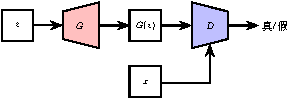
\includegraphics[width=.8\textwidth]{figs/GAN.pdf}
	\caption{GAN模型示意图\cite{goodfellow2014generative}。}
	\label{GAN}
\end{figure}

生成对抗网络相比较其它生成模型,优点在于:只用到了反向传播和梯度下降;可生成更逼真的样本;在应用方面,因其是非配对的训练方式,所以可以很自然地应用到无监督和半监督学习中;在设计损失函数方面,对于图像超分辨率、图像修复、图像去噪和风格迁移等任务上,无需根据任务的不同去精心设计损失函数,只需要给定想要达到的基准图像即可,判别器自会尽力生成高质量图像,避免了损失函数的设计困难。但生成对抗网络也有其缺点:因在训练时需要交替训练生成器和判别器,所以容易造成训练不稳定,难以达到纳什平衡;在训练时,判别器训练得比生成器快,当判别器训练得很好时,能很容易区别出真实样本和生成样本,从而出现梯度消失的问题;当生成器生成的样本仅代表真实样本的部分模式就可以欺骗判别器时,会导致生成样本缺乏多样性,出现模式崩塌。针对GAN存在的一系列问题,研究者们在GAN的基础上提出了各种变体或训练技巧加以避免。

\section{生成对抗网络变体}

GAN自提出后大受追捧,虽然可以生成比其它生成模型更清晰的图像,但仍存在一些问题,如:(1)生成器和判别器训练程度不对等,判别器训练得快且好,导致训练初期生成器的梯度容易消失,进而使生成器的参数基本不会更新;(2)训练不稳定,容易出现模式崩塌,生成器产生无意义的输出。研究者考虑GAN存在的问题以及可挖掘的空间,提出一系列GAN的变体模型。

\subsection{条件生成对抗网络}

原始GAN的输入是随机噪声,且无需预先建模,因此无法控制生成器的输出,2014年Mirza等人\cite{mirza2014conditional}提出的条件生成对抗网络(CGAN)在GAN的基础上给$G$和$D$加入额外的条件变量$y$,$y$在此起到约束和指引的作用,使生成样本可控。

\begin{figure}[ht]
    \centering
	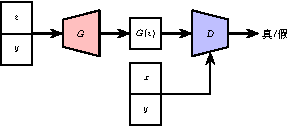
\includegraphics[width=.8\textwidth]{figs/CGAN.pdf}
	\caption{CGAN模型示意图\cite{mirza2014conditional}。}
	\label{CGAN}
\end{figure}

当加入条件变量$y$后,CGAN的目标函数为:
\begin{equation}
\begin{split}
\min \limits_{G} \max \limits_{D} V(D,G) = \mathbb{E}_{x\sim p_{data}(x)}[\log D(x|y)] + \mathbb{E}_{z\sim p_z(z)}[\log(1 - D(G(z|y)))]
\end{split}
\label{eq:CGAN}
\end{equation}

具体来说(如图\ref{CGAN}所示),假如$y$为类别标签,先将$y$进行one-hot编码,然后与随机噪声$z$按通道拼接,拼接后的编码输入生成器,得生成图像$G(z|y)$,判别器也用相似的处理方式将真实样本$x$或生成样本$G(z|y)$与$y$融合,判别器的输出$D(x|y)$或$D(G(z|y))$表明输入图像为真或假的概率。



\subsection{深度卷积生成对抗网络}

GAN中G和D的网络结构由简单的全连接层构成,存在难以训练的问题,深度卷积生成对抗网络(DCGAN)主要从网络结构上对GAN做改进。卷积神经网络(CNN)的开山之作是LeNet-5\cite{lecun1998gradient},在2012年ImageNet比赛上凭借AlexNet\cite{krizhevsky2012imagenet}大放异彩,从此广泛应用于计算机视觉领域。2016年Radford等人\cite{radford2015unsupervised}提出深度卷积生成对抗网络,将CNN引入$G$和$D$的网络结构中(如图\ref{DCGAN}),因为CNN之前多用于监督学习任务,而GAN是无监督学习,直接用卷积层替换全连接层并不能保证训练正常进行,经过探索,DCGAN确定了一个可以保证训练正常进行的方案:

(1)$G$和$D$中没有池化层和上采样层,转而用带步长的卷积代替,具体分为$D$用步长卷积,$G$中用反卷积,以提高训练的稳定性;

(2)在$G$和$D$中几乎每一层都用到批归一化(BN\cite{ioffe2015batch}),防止$G$把所有样本收敛到一个点,但直接将BN应用到所有层会导致模型不稳定,因此$G$的最后一层和$D$的第一层不加BN;

(3)移除全连接隐藏层,以构建更深层网络;

(4)$G$中使用$ReLU$\cite{nair2010rectified}激活函数,除了最后一层采用的是$Tanh$激活函数;

(5)$D$中所有层采用$LeakyReLU$\cite{xu2015empirical}激活函数。

DCGAN提出的网络结构不仅能够稳定训练,还能生成高质量图像,同时学习有意义的分解表示,可用于监督学习和生成建模。

\begin{figure}[ht]
    \centering
	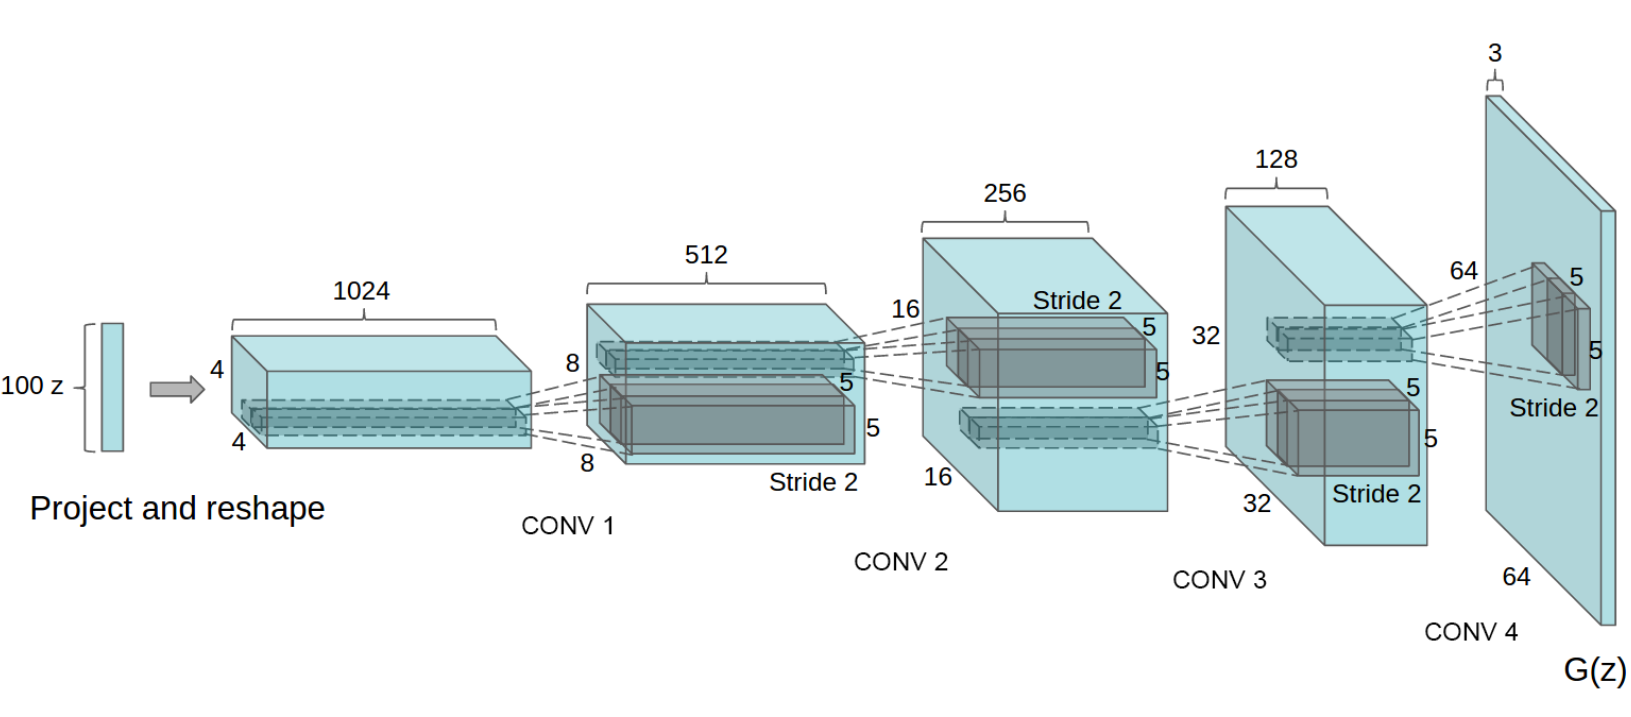
\includegraphics[width=\textwidth]{figs/DCGAN.png}
	\caption{DCGAN生成器结构示意图。图片来自文献\cite{radford2015unsupervised}。}
	\label{DCGAN}
\end{figure}

\subsection{结合变分自编码器的生成对抗网络}

VAE-GAN\cite{larsen2016autoencoding}提出了一种结合变分自编码器的生成对抗网络,如果只用VAE\cite{kingma2013auto}生成图像,容易产生模糊的结果,但生成结果有较高的多样性,如果只用GAN\cite{goodfellow2014generative},虽然能提高生成质量,但容易模式崩塌。VAE-GAN充分发挥这两种生成模型的优势,如图\ref{VAE-GAN}所示,VAE中的编码器将输入图像编码为均值和方差,利用均值和方差得到一个分布,并从此分布中采样得隐向量$z$,$z$经解码器生成$G(z)$。VAE的损失函数由两部分组成:确保生成图像和输入图像有一定相似性的损失和保证隐向量服从高斯分布的损失。VAE-GAN将VAE用作GAN的生成器,再加入一个判别器,用于判别输入图像的真假,VAE-GAN损失函数为VAE和GAN的损失函数之和。实验证明,VAE-GAN的生成效果比单独使用VAE或GAN好。

\begin{figure}[ht]
    \centering
	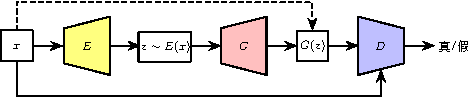
\includegraphics[width=\textwidth]{figs/VAEGAN.pdf}
	\caption{VAE-GAN模型示意图\cite{larsen2016autoencoding}。}
	\label{VAE-GAN}
\end{figure}

\section{基于生成对抗网络的图像翻译}

\subsection{配对图像翻译}
2017年Isola等人\cite{isola2017image}提出了基于条件生成对抗网络的图像翻译模型pix2pix,如图\ref{pix2pix}所示,整个网络架构中只有一个生成器$G$和一个判别器$D$,源域图像$x$经生成器$G$得生成的目标域图像$G(x)$,在判别时,源域图像作为条件辅助判别,其对抗损失函数类似于CGAN。

在pix2pix中,判别器的目的没有变化,但生成器的目的不仅是骗过判别器,还需要和真实图像尽可能相似,L1损失\cite{isola2017image}\cite{shrivastava2017learning}(公式\ref{eq:pix2pix_l1})相比较L2损失\cite{pathak2016context}可以在保证与真实图像相近的同时产生更少的模糊。
\begin{equation}
\begin{split}
\mathcal{L}_{L1}(G) = \mathbb{E}_{x,y,z}[\parallel y-G(x,z)\parallel_1]
\end{split}
\label{eq:pix2pix_l1}
\end{equation}

\begin{figure}[ht]
    \centering
	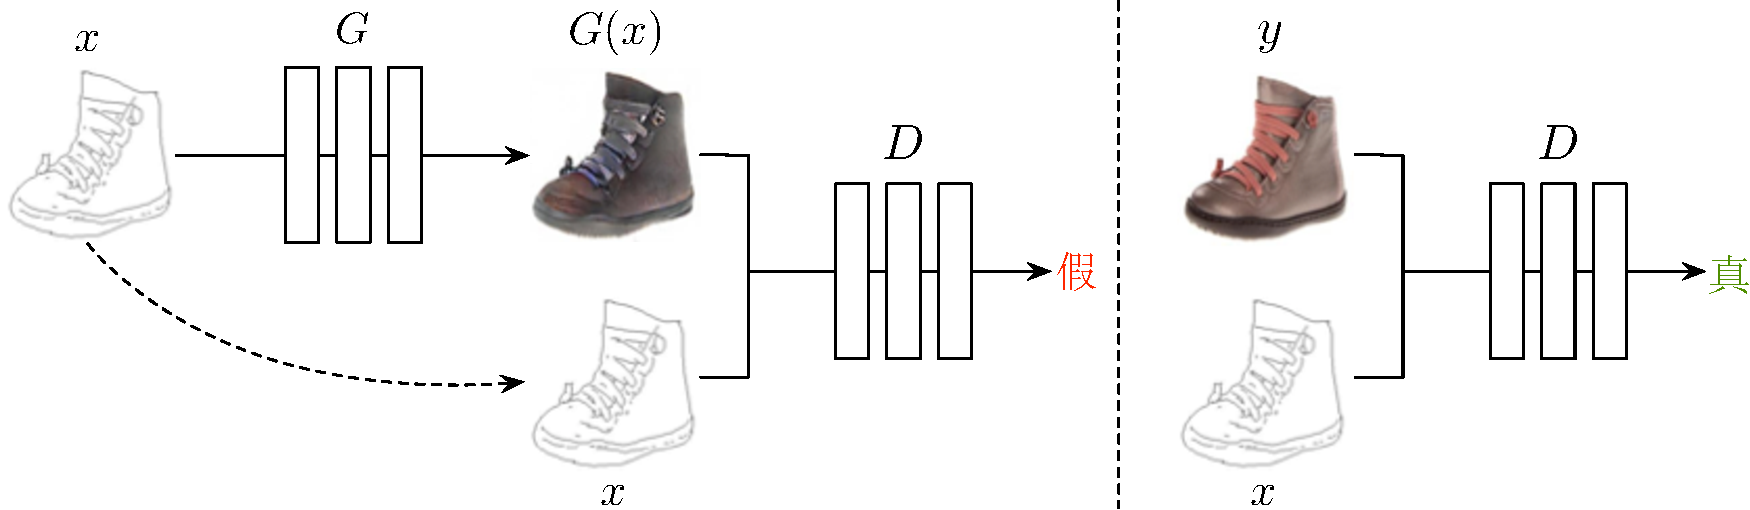
\includegraphics[width=\textwidth]{figs/pix2pix.pdf}
	\caption{Pix2pix训练示意图。图片来自文献\cite{isola2017image}。}
	\label{pix2pix}
\end{figure}

Isola等人认为虽然输入图像和输出图像外观上不同,但潜在结构应相似,输入和输出之间共享大量低级信息,因此生成器采用有跳连接的U-Net\cite{ronneberger2015u}结构,下采样过程中产生的特征图与上采样过程产生的同尺寸的特征图按通道拼接到一起,以此保留不同分辨率的信息,提高生成质量。Pix2pix的目标函数包含学习低频信息的重建损失和学习高频信息的对抗损失,既然对抗损失只解决高频信息,所以判别器采用的是PatchGAN结构,它不需要将整幅图像输入到判别器中,而是对每个大小为N$\times$N的区域做真假判别。

\begin{figure}[ht]
    \centering
	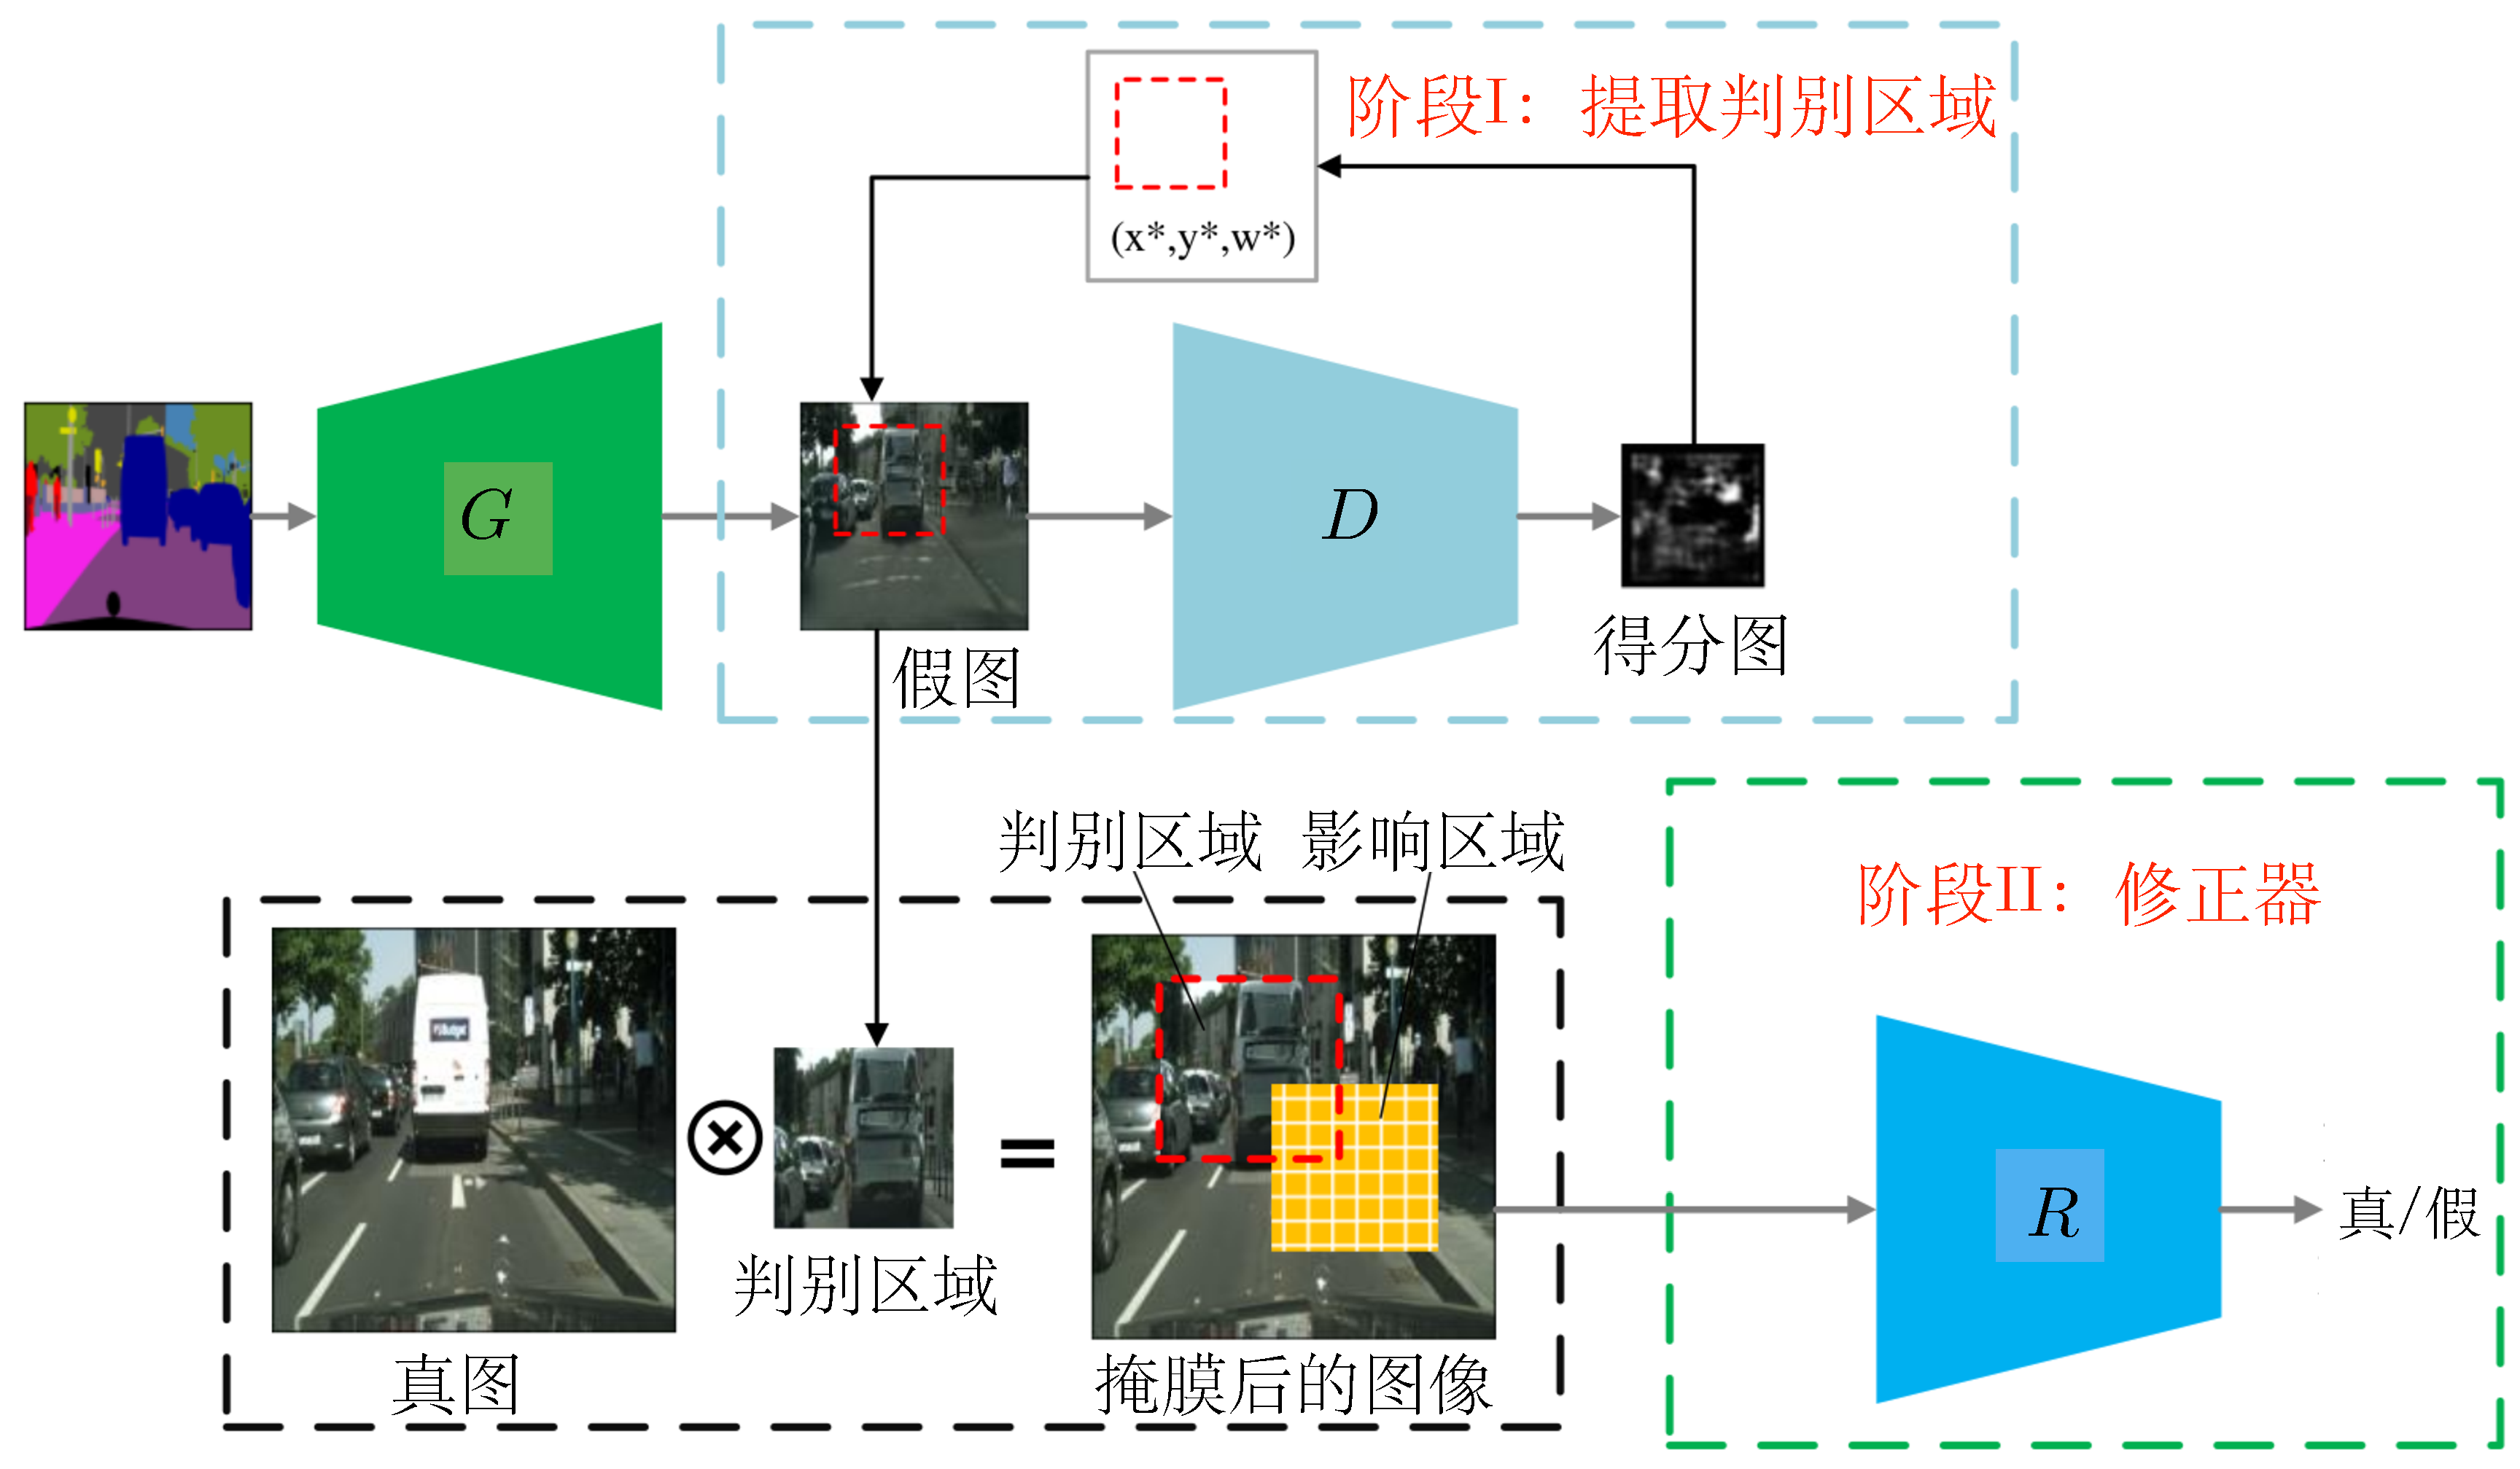
\includegraphics[width=.9\textwidth]{figs/DRPAN.pdf}
	\caption{DRPAN训练示意图。图片来自文献\cite{wang2019discriminative}。}
	\label{DRPAN}
\end{figure}

Wang等人\cite{wang2019discriminative}考虑图像翻译任务中仍存在的失真、形变和拉伸等问题,提出DRPAN以得到高质量和高分辨率的图像翻译结果。如图\ref{DRPAN}所示,整个网络由三部分组成:生成器$G$、判别器$D$和修正器$R$。输入图像经生成器得到假图,随后假图进入判别器,此判别器在PatchGAN的基础上扩展为一个判别区域建议网络,主要用于输出反映生成图像真实程度的得分图,然后通过滑动窗口找到并提取假图中得分较低的区域,即图\ref{DRPAN}中的判别区域。判别区域与真图做掩膜操作得到掩膜后的假图,然后将真图和掩膜后的假图输入修正器中做优化训练,修正器可以对一幅图像不同的区域进行迭代式更新优化。将掩膜后的图像输入修正器的行为可看作一种直接的注意力机制,让修正器专注于修正合成效果不好的位置。

SPADE\cite{park2019semantic}提出一个简单但有效的层:空间自适应归一化,可用于将语义分割图翻译成图像。之前的工作是将语义分割图作为输入直接喂入网络中,然后通过卷积层、归一化层和非线性激活函数处理,但这易于“冲走”语义信息。为了解决此问题,SPADE提出了空间自适应归一化,用学习到的缩放和偏差进行调制。输入图像经编码器得到与其分布有关的均值和方差,然后利用此均值和方差与高斯分布进行反归一化,得到一个包含真实图像信息的随机向量,生成器以随机向量为输入,并在此过程中不断加入语义分割图以利用SPADE增强语义信息,最终得到逼真的图像。

虽然上述方法可以生成高质量图像,但它需要配对数据集,而配对数据集的获取十分困难,而且对于一些任务,获取配对数据集是不可能的,如照片转莫奈画,马转斑马等,因此需要一种可以实现非配对图像翻译的方法。

\subsection{非配对图像翻译与循环一致}

Zhu等人\cite{zhu2017unpaired}提出的CycleGAN能够在没有配对数据的情况下,在源域和目标域之间建立一个确定的映射,实现图像翻译。给定源域$X$和目标域$Y$,利用生成器$G$学习从$X$到$Y$的映射$G:X\to Y$,即给定来自$X$域的图像$x$,经此映射可得$Y$域的生成图像$\hat{y}=G(x)$,理论上,$\hat{y}$应与真实样本的分布$p_{data}(y)$相匹配,最优$G$将图像从$X$域翻译到与$Y$域相近的$\hat{Y}$域,但实际上,由于缺乏配对数据集提供的约束,$G:X\to Y$映射并不能保证输入$x$与输出$y$以有意义的方式配对,即无法保证$G$是单一的,这容易导致模式崩塌。针对这一问题,zhu等人提出再增加一个映射$F:Y\to X$,$G$和$F$的网络结构一致,除此之外,还引入循环一致性损失用于确保$F(G(x)) \approx x$和$G(F(y)) \approx y$,损失函数定义为:
\begin{equation}
\begin{split} 
\mathcal{L}_{cyc}(G, F) = \mathbb{E}_{x\sim p_{data}(x)}[\parallel F(G(x)) - x\parallel_1] + \mathbb{E}_{y\sim p_{data}(y)}[\parallel G(F(y)) - y\parallel_1]
\end{split}
\label{eq:pix2pix}
\end{equation}
与两个生成器相对应,CycleGAN还引入有相同结构的判别器$D_X$和$D_Y$,用于对$X$域和$Y$域的判别,总损失函数是循环一致性损失和对抗损失的和。

\begin{figure}[ht]
    \centering
	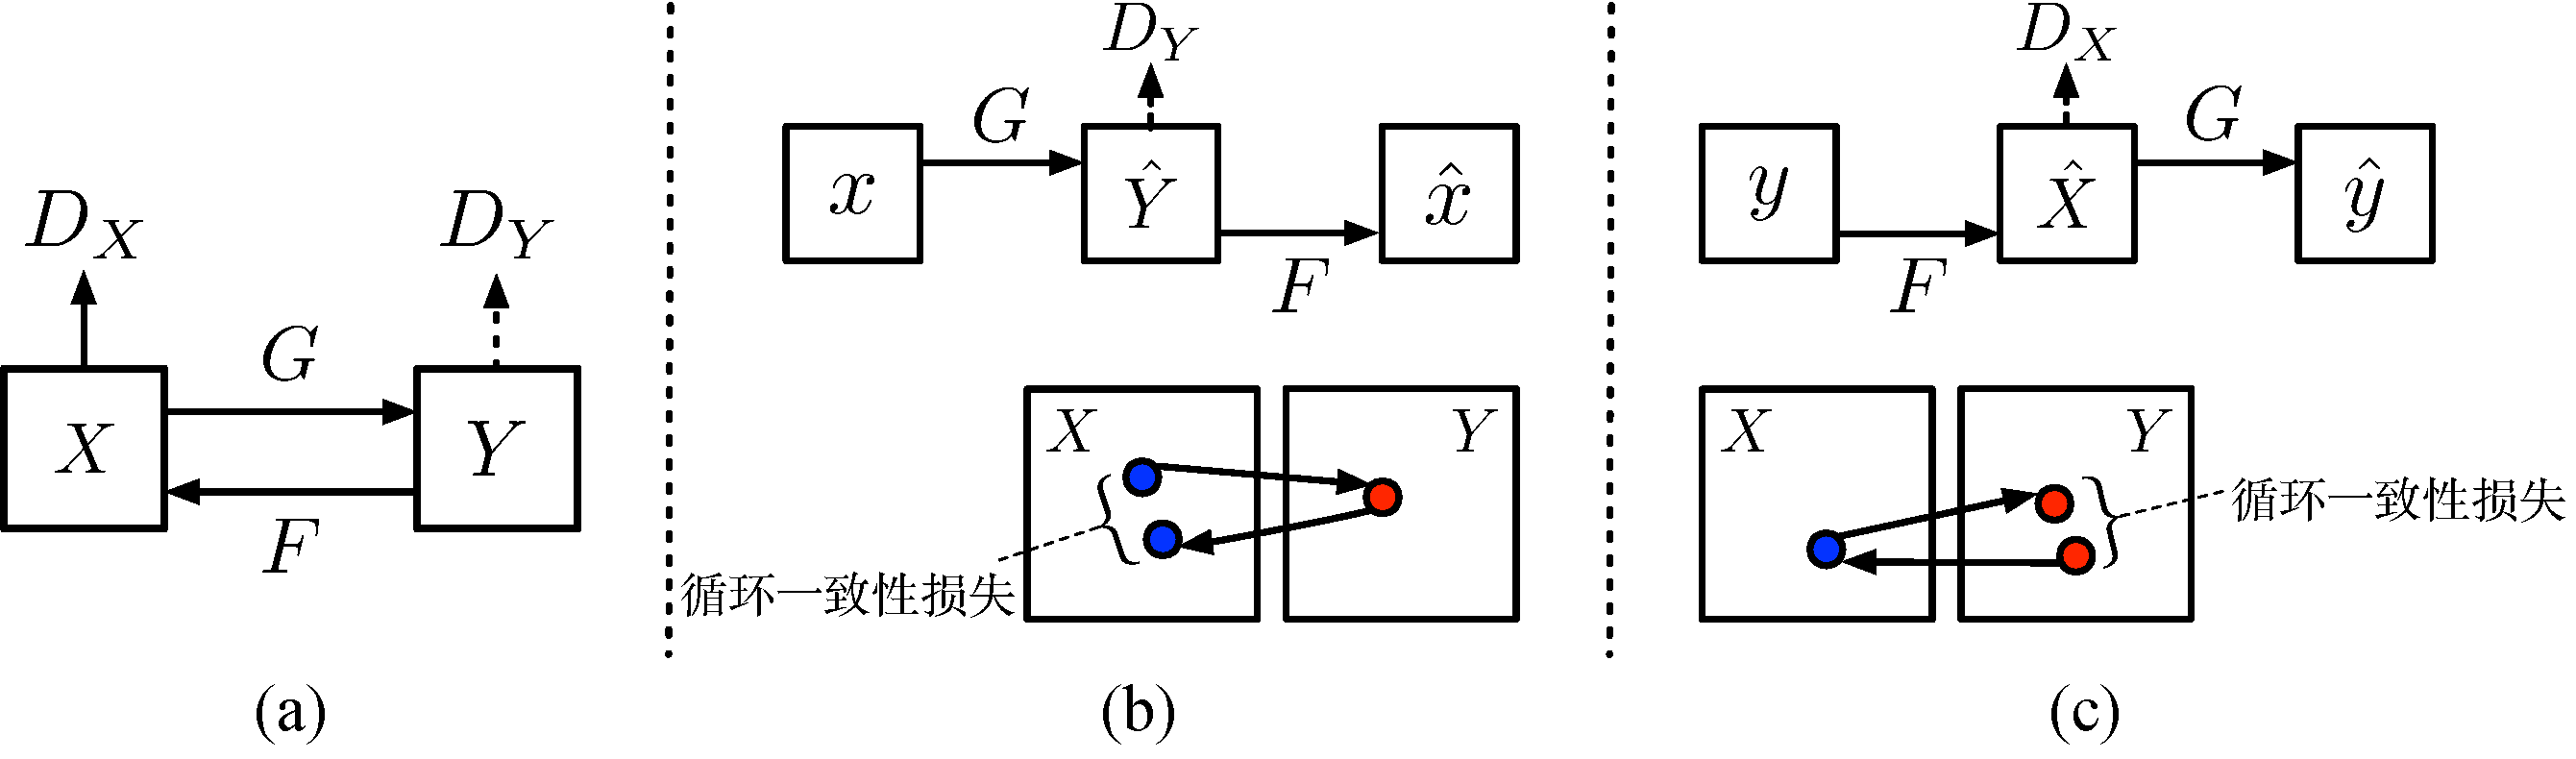
\includegraphics[width=\textwidth]{figs/cyclegan.pdf}
	\caption{CycleGAN训练示意图。图片来自文献\cite{zhu2017unpaired}。}
	\label{CycleGAN}
\end{figure}

CycleGAN在马和斑马、季节变化、照片和画作等任务上均性能优异,验证了CycleGAN的广泛适用性和有效性。使用循环一致性损失的还有Kim等人\cite{kim2017learning}提出的DiscoGAN和Yi等人\cite{yi2017dualgan}提出的DualGAN,它们的方法和思想类似,此处不再展开介绍。

Liu等人提出的UNIT\cite{liu2017unsupervised}将非配对图像翻译定义为知道边缘概率密度,学习联合概率密度的问题,但这是一个高度不适定问题,对此,UNIT提出一种共享潜在空间的假设。假定$X_1$和$X_2$分别表示两个图像域,图像$x_1\in X_1$和$x_2\in X_2$可分别经过编码器$E_1$和$E_2$被映射到相同的潜码$z$,生成器$G_1$和$G_2$可再将潜码$z$解码回相应的$x_1$和$x_2$。为了实现共享潜在空间,UNIT利用权重共享策略,将编码器的后几层连接到一起,生成器的前几层也连接到一起。UNIT在白天转黑夜、动物脸翻译等任务上表现较好,但它的输出只能是单模态的,不能实现一对多翻译。

\subsection{非配对图像翻译与分解表示}

Huang等人提出的MUNIT\cite{huang2018multimodal}将一幅图像分解到代表底层空间结构的内容隐空间和代表结构渲染的风格隐空间,文中假设两个域共享同一个内容隐空间,风格隐空间是特定于域的,如\ref{MUNIT}所示,$x_1 \in X_1$和$x_2 \in X_2$是来自两个域的图像,$c_i$和$s_i$分别是由$x_i$经两个编码器得到的内容隐编码和风格隐编码。为了实现从$X_1$到$X_2$域的翻译,MUNIT将提取的内容隐编码$c_1=E_1^c(x_1)$和从先验分布$q(s_2)\sim\mathcal{N}(0, \mathbf{I})$中随机采样的风格隐编码输入到生成器$G_2$中,以产生最终的输出图像$x_{1\to2}=G_2(c_1,s_2)$。

\begin{figure}[ht]
    \centering
	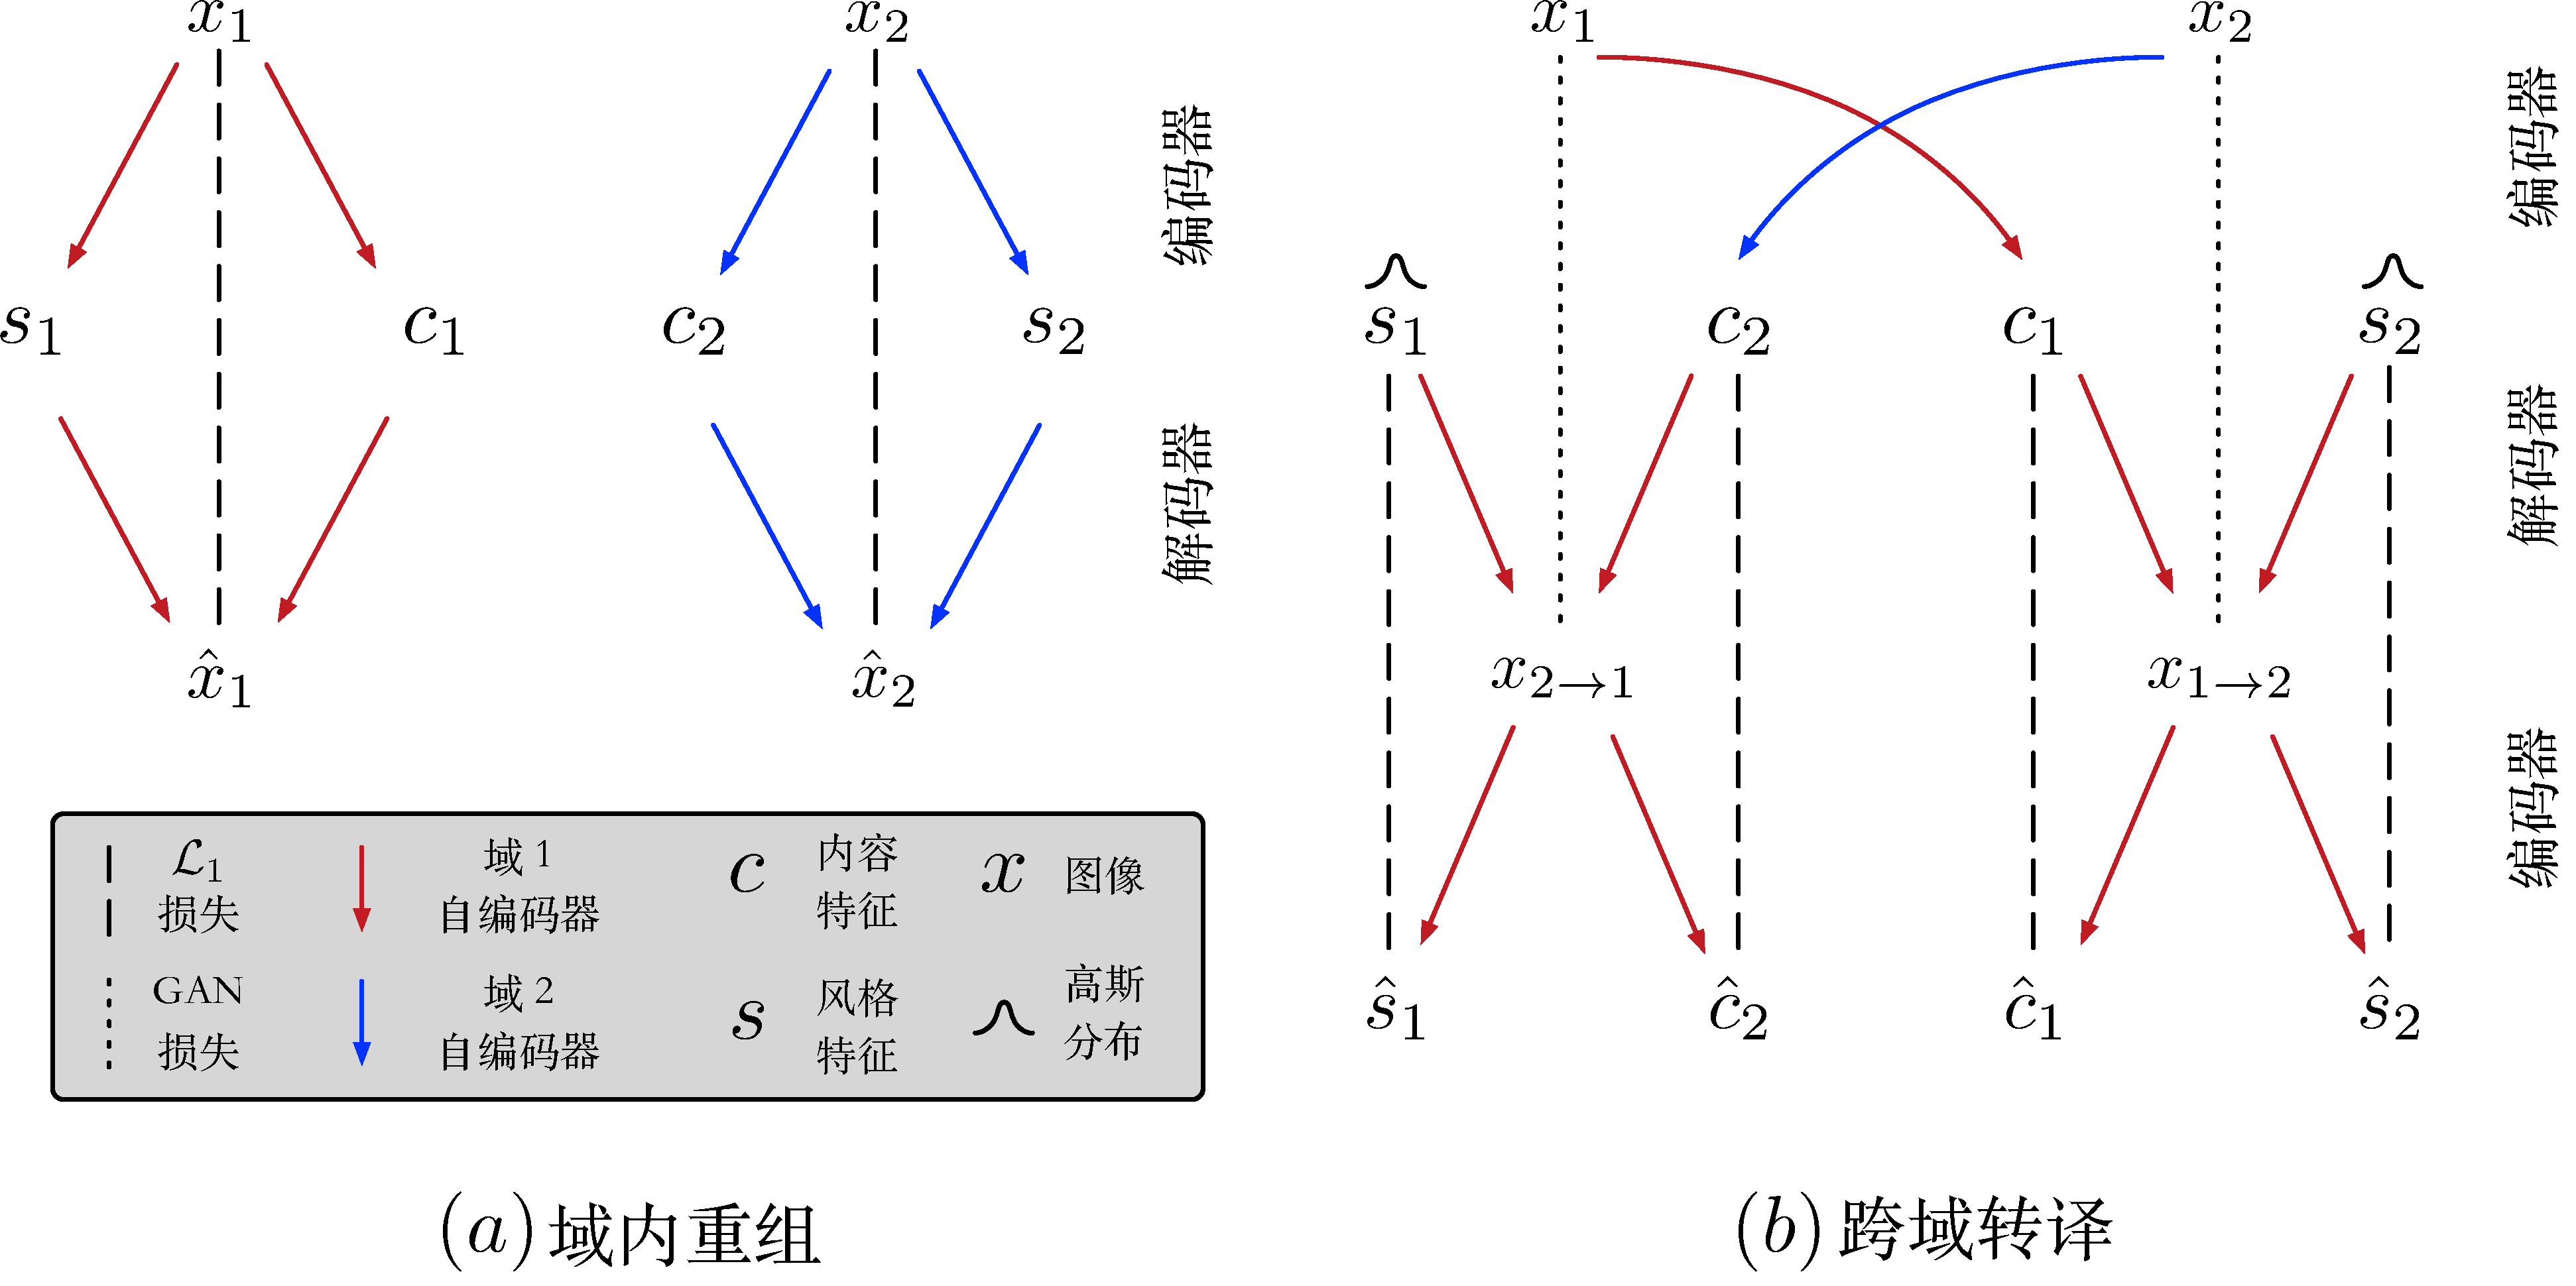
\includegraphics[width=\textwidth]{figs/MUNIT.pdf}
	\caption{MUNIT训练示意图。图片来自文献\cite{huang2018multimodal}。}
	\label{MUNIT}
\end{figure}

MUNIT的损失函数包括对抗损失和双向重建损失,对抗损失使生成图像的分布尽量逼近目标域的图像分布,双向重建损失则用于确保配对的编码器和解码器互逆。双向重建损失包含对图像的重建和对潜码的重建:给定一个源域图像,经过编码和解码后可重建出此源域图像;给定一个从潜在空间采样的潜码,经过解码和再次编码,应该重建出此潜码。

Lee等人提出的DRIT\cite{lee2018diverse}与MUNIT类似,也假设有一个捕捉不同域之间共同信息的域不变内容隐空间和两个特定于域的属性隐空间,图\ref{DRIT}中的$\{E_X^c, E_Y^c\}$和$\{E_X^a, E_Y^a\}$分别为两个域的内容编码器和属性编码器,$G_X$和$G_Y$是生成器,用于将内容隐编码和属性隐编码整合并生成图像。

为了实现分解表示,将两个内容编码映射到同一隐空间中,DRIT采用权重共享和内容判别策略,共享$E_X^c$和$E_Y^c$的最后一层以及$G_{X}$和$G_{Y}$的第一层权重,通过权重共享,将内容表示强制映射到同一空间。但共享相同的高级映射函数并不能保证可将不同域的内容表示成相同的内容编码,因此还引入用于判别内容编码$z_x^c$和$z_y^c$的判别器$D^c$。

\begin{figure}[ht]
    \centering
	\includegraphics[width=\textwidth]{figs/DRIT.pdf}
	\caption{DRIT训练示意图。图片来自文献\cite{lee2018diverse}。}
	\label{DRIT}
\end{figure}

MUNIT和DRIT都采用分解表示的方式实现多模态输出,是多模态图像翻译方面的经典之作,后续产生一系列在它们基础上改进的工作。Mao等人提出的MSGAN\cite{mao2019mode}设计了一个简单但有效的模式搜寻正则化项,其主要思想是最大化输出图像之间的距离与输入的隐空间之间的距离的比值,可解决CGAN模式崩塌问题。这一正则化项很容易扩展到现有框架中,在非配对图像翻译中,MSGAN在DRIT上加入模式搜寻正则化项,可得到更多样和更高质量的图像。

给定一个来自隐编码空间$Z$的隐向量$z$,将其映射到图像空间$I$中,当网络发生模式崩塌时,输出图像只有少量模式,即当两个隐向量$z_1$和$z_2$很接近时,映射得到的两个图像$I_1=G(c,z_1)$和$I_2=G(c,z_2)$更趋向于有相同的模式。为解决此问题,MSGAN提出模式搜寻正则化项,旨在最大化$G(c,z_1)$和$G(c,z_2)$之间的距离与$z_1$和$z_2$之间的距离的比值:
\begin{equation}
\begin{split} 
\mathcal{L}_{ms}=\max\limits_{G}(\frac{d_I(G(c,z_1),G(c,z_2))}{d_z(z_1,z_2)}),
\end{split}
\label{eq:MSGAN}
\end{equation}
其中$d_{\ast}(\cdot)$表示距离度量。相比于DRIT从高斯分布中采样一个编码,为将模式搜寻正则化加入DRIT中,现从高斯分布中随机采样两个编码$z_1$和$z_2$,仅做一点改变就可输出更多样化的结果。

\begin{figure}[ht]
    \centering
	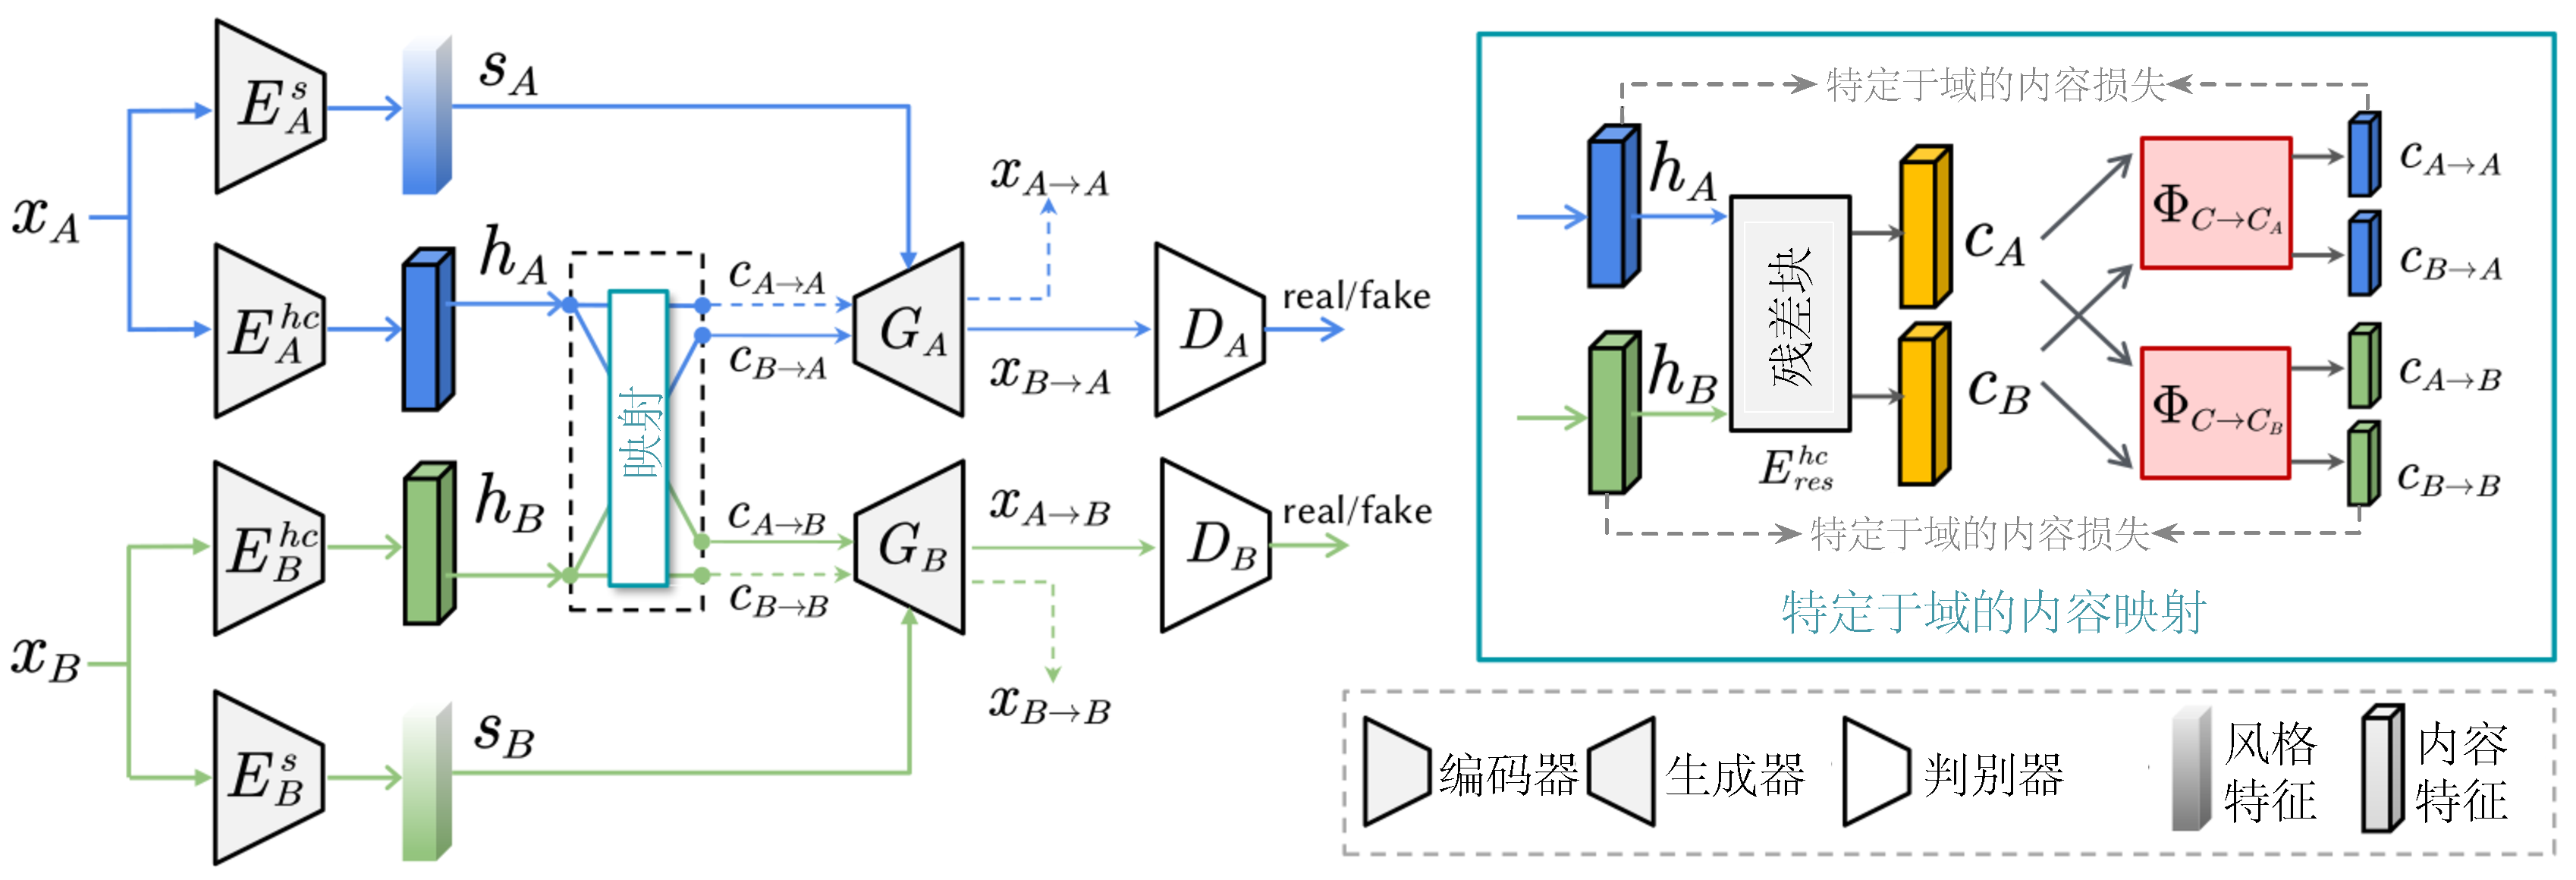
\includegraphics[width=\textwidth]{figs/DSMAP.pdf}
	\caption{DSMAP训练示意图。图片来自文献\cite{chang2020domain}。}
	\label{fig:DSMAP}
\end{figure}

Chang等人\cite{chang2020domain}提出的DSMAP在MUNIT的基础上,对共享的域不变内容空间中的潜在特征做进一步映射(如图\ref{fig:DSMAP}所示),将其重新映射到特定于域的内容空间中。DSMAP做此改进是因为作者观察到之前基于分解的方法不考虑内容和风格之间的关系,共享的域不变内容空间可能会限制表达内容的能力,因为域不变的内容特征可能包含域相关信息。

在两个域$X_A$和$X_B$中,除了基本的内容编码器$\{E_A^c, E_B^c\}$、风格编码器$\{E_A^s, E_B^s\}$和生成器$\{G_A, G_B\}$,DSMAP还引入两个额外的特定于域的映射函数$\Phi_{C\to C_A}$和$\Phi_{C\to C_B}$,它们将共享的域不变内容空间中的特征映射到特定于$X_A$域和$X_B$域的内容空间中。在$X_A\to X_B$的翻译中,内容来自于$X_A$,风格来自于$X_B$,内容编码器$E_A^c$将$x_A\in X_A$映射到为域不变内容特征$c_A=E_A^c(x_A)$,风格编码器$E_B^s$将$x_B\in X_B$映射到为特定于域的风格特征$s_B=E_B^s(x_B)$,MUNIT和DRIT通过生成器$G_B$得生成图像$x_{A\to B}=G_B(c_A, s_B)$。DSMAP认为这样简单地提取域不变内容特征$c_A$不足以生成高质量$X_B$域图像,最好在合成前就将$c_A$和目标域的内容特征对齐。因此,$\Phi_{C\to C_B}$将内容特征$c_A$映射到$X_B$的内容空间,然后生成器$G_B$利用内容特征$c_{A\to B}$和风格特征$s_B$合成最终的输出图像$x_{A\to B}$。总的来说,$X_A\to X_B$的生成过程为:
\begin{equation}
\begin{split} 
x_{A\to B}=\Phi_{X_A\to X_B}(x_A, x_B)=G_B(\Phi_{C\to C_B}(c_A), s_B),
\end{split}
\label{eq:DSMAP}
\end{equation}
DSMAP提出了一种分解特征再映射的想法,其可以提取更纯净的内容特征的特点使之在风格迁移任务上展示出更有说服力的结果。

\section{小结}

本章从生成对抗网络的原理展开,介绍了不同的生成对抗网络变体和多种基于生成对抗网络的图像翻译方法。

第一节主要介绍了生成对抗网络的原理和主要架构,指出GAN以博弈的方式提高了生成质量,但也伴随着模式崩塌、训练不稳定、生成图像的分辨率不高和生成样本多样性不足等问题。

第二节介绍了GAN的一系列变体,DCGAN和VAE-GAN等通过提出新的网络架构以保证GAN可以稳定训练,在一定程度上缓解了模式崩塌。

第三节介绍基于生成对抗网络的图像翻译方法,然后分析了配对图像翻译(包括pix2pix等)和非配对图像翻译(包括CycleGAN和DRIT等),重点介绍非配对图像翻译中的两种思想:循环一致和分解表示。

在逐步地深入介绍后,明确基于生成对抗网络的图像翻译的原理和应用,接下来将关注非配对图像翻译,利用循环一致和分解表示解决两个应用问题。
\chapter{基于生成对抗网络的多目标形变图像翻译}

\section{引言}

图像翻译旨在学习从一个图像域到另一个图像域的映射,可广泛应用于图像着色、超分辨率和风格迁移等任务中,非配对图像翻译如CycleGAN\cite{zhu2017unpaired}和DiscoGAN\cite{kim2017learning}等可以通过使用生成对抗网络进行深度学习,使用循环一致性损失来解决缺少配对数据集的问题,能够在马和斑马、苹果和橘子等数据集上取得较好的效果,实现在图像域之间传递复杂的局部纹理外观。图\ref{fig:cyclegan_failure}展示了CycleGAN无法实现狗转猫或者猫转狗的翻译,这是因为猫和狗两个域之间不仅存在纹理上的差异,还存在形状上的不同,这对之前的图像翻译方法来说具有挑战性。

\begin{figure}[ht]
    \centering
	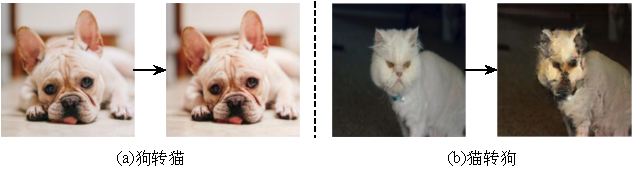
\includegraphics[width=\textwidth]{figs/cyclegan_failure.pdf}
	\caption{CycleGAN在有较大形状差异数据集上的翻译结果。图片来自文献\cite{zhu2017unpaired}。}
	\label{fig:cyclegan_failure}
\end{figure}

当图像中仅存在一个需要做形变翻译的目标,我们称此类任务为单目标形变图像翻译,近年来一些工作如U$-$GAT$-$IT\cite{kim2019u}、TransGaGa\cite{wu2019transgaga}等聚焦于单目标形变图像翻译,利用注意力机制或几何信息等方式取得令人满意的结果。但很多时候,图像中的目标并非一个,而是多个目标同时存在,如野外环境中多只羊翻译为多只长颈鹿,本节的工作即做此任务,称为多目标形变图像翻译,在实现形变的同时思考如何处理多个目标的图像翻译。为了解决此问题,我们将形状、纹理和背景分开处理,并利用第二节提到的循环一致性思想,提出一个基于生成对抗网络的模型,最终实现具有较大形状变化的多目标图像翻译,从而可以将图像翻译的实用性提高到一个新的水平。

\section{模型算法}

多目标形变图像翻译需要考虑的问题有两个:(1)如何确定每个目标;(2)如何实现形变。受InstaGAN\cite{mo2018instagan}启发,我们利用实例分割图确定每个目标的位置和形状,获得多个目标的实例信息。在探索过程中发现(如图\ref{fig:mask}),对于同样的网络,当在两个图像域之间翻译时,难以实现形状变化,但当在两个实例分割域之间做翻译时,可以实现形状的变化,因此我们提出将背景、形状和纹理分开处理。利用实例分割图实现两个域中多个目标在形状上的翻译,然后学习图像域的纹理特征,向翻译后的形状增添纹理信息,得到完整的翻译后的前景目标,再将此前景目标与背景结合,并经过一个细化网络,最终实现多目标形变图像翻译。

\begin{figure}[ht]
    \centering
	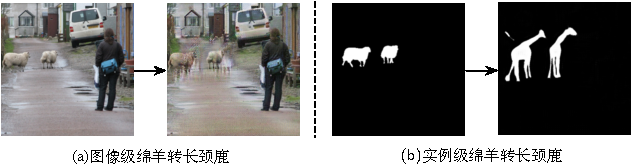
\includegraphics[width=\textwidth]{figs/mask.pdf}
	\caption{图像级和实例级的绵羊转长颈鹿结果。}
	\label{fig:mask}
\end{figure}

\subsection{算法框架}

给定两个图像域$X$和$Y$,并规定其对应的实例域为$M_X$和$M_Y$,对于图像$x\in X$和其对应的实例分割图$m_x\in M_X$,我们的任务是在保持其背景不变的情况下,将目标的形状和纹理翻译至$Y$域。我们将此问题分为四个部分:形状翻译、纹理翻译、背景翻译和进一步处理融合图像的细化网络,下面将详细介绍。

\begin{figure}[ht]
    \centering
	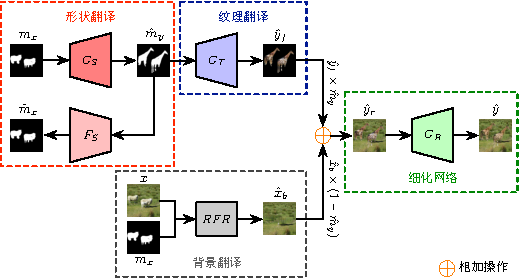
\includegraphics[width=\textwidth]{figs/multi_instance.pdf}
	\caption{多目标形变图像翻译模型示意图。}
	\label{fig:multi_instance}
\end{figure}

\subsubsection{形状翻译}

如图\ref{fig:multi_instance}中红色虚线框部分所示,我们在两个实例分割域之间进行翻译,因训练所用的数据集不配对,所以我们采用循环一致\cite{zhu2017unpaired}的训练方式。给定两个域$M_X$和$M_Y$,我们的目标是学习两个域之间的映射:$G_S: M_X\to M_Y$和$F_S: M_Y\to M_X$,实例分割图$m_x\in M_X$经生成器$G_S$合成$\hat{m}_y=G_S(m_x)$,并利用判别器$D_{S_y}$区分$\hat{m}_y$和$m_y\in M_Y$,然后利用生成器$F_S$将$\hat{m}_y$翻译为重建图像$\tilde{m}_x$,并约束$F_S(G_S(m_x))\approx m_x$使重建图像与输入图像接近。

\subsubsection{纹理翻译}

给定经过形状翻译的实例分割图$\hat{m}_y$,在纹理翻译部分的目的是向$\hat{m}_y$上添加属于$Y$域的纹理(如图\ref{fig:multi_instance}中蓝色虚线框部分所示),它要求网络可以准确定位到需要添加纹理的位置并学习需添加的纹理样式。类似于文献\cite{yang2019controllable},我们将此问题看作:给定配对数据\{$m_y$, $y$\},其中$y$为来自Y域的图像,$m_y\in M_Y$是与$y$相对应的实例分割图,训练一个纹理生成器$G_T$,使之可以学习映射$G_T: M_Y\to Y$。需要提到的一点是,因为我们希望网络仅学习实例分割图中标注的部分,因此为了更精准地训练和学习,排除其它位置的信息对纹理生成器的影响,我们仅取出$y$中与$m_y$相对应的部分(记作$y_f$)看作真实图像,因此判别器$D_T$对生成图像$\hat{y}_f=G_T(\hat{m}_y)$和真实图像$y_f$进行判别。

\subsubsection{背景翻译}

因为做图像翻译的两个域在形状上相差较大,如果直接用生成的目标替代原本的目标,那么在生成图像中很容易出现生成目标的周围还残留部分原目标内容的情况,使整个图像看起来不和谐。得益于图像修复的发展,我们利用一个图像修复算法RFR\cite{li2020recurrent}将图像$x$中与$m_x$相对应的部分进行修复,得到一个相对完整的背景$\hat{x}_b$。

\subsubsection{细化网络}

经过前面三个部分的训练,我们现在可以得到经过形状翻译的实例分割图$\hat{m}_y$、经过纹理翻译的前景目标$\hat{y}_f$和经过背景翻译的背景$\hat{x}_b$,利用公式\ref{eq:refine}将这三部分融合到一张图像中,即图\ref{fig:multi_instance}绿色虚线框部分中的$\hat{y}_r$,此时的融合图像存在前景目标与背景之间衔接不自然以及纹理部分生成粗糙等问题,为了解决这些问题,我们引入一个细化生成器$G_R$,得到最终的生成图像$\hat{y}=G_R(\hat{y}_r)$。
\begin{equation}
\begin{split}
\hat{y}_r=\hat{y}_f\times\hat{m}_y+\hat{x}_b\times(1-\hat{m}_y)
\end{split}
\label{eq:refine}
\end{equation}

\subsection{目标函数}

\subsubsection{形状翻译}

我们的目标函数有两项:用于将生成图像的分布尽量逼近目标域中的数据分布的对抗损失\cite{goodfellow2014generative}和防止学习到的映射$G_S$与$F_S$相矛盾的循环一致性损失\cite{zhu2017unpaired}。对于映射$G_S: M_X\to M_Y$和相应的判别器$D_{S_y}$,我们定义对抗损失为:
\begin{equation}
\begin{split}
\mathcal{L}_{adv\_x}^{shape}=\mathbb{E}_{m_y}[\log D_{S_y}(m_y)] + \mathbb{E}_{m_x}[\log(1-D_{s_y}(G_S(m_x))]
\end{split}
\label{eq:shape_x}
\end{equation}
其中生成器$G_S$的目的在于使生成的图像看起来属于$M_Y$域,而判别器$D_{S_y}$旨在分辨出生成器合成的图像$\hat{m_y}$和真实图像$m_y$。对于映射$F_S: M_Y\to M_X$和判别器$D_{S_x}$,我们定义此方向的对抗损失为:
\begin{equation}
\begin{split}
\mathcal{L}_{adv\_y}^{shape}=\mathbb{E}_{m_x}[\log D_{S_x}(m_x)] + \mathbb{E}_{m_y}[\log(1-D_{s_x}(F_S(m_y))]
\end{split}
\label{eq:shape_y}
\end{equation}
其中生成器$F_S$和判别器$D_{S_x}$的目的分别与$G_S$和$D_{S_y}$类似。将两个方向的对抗损失合并,得完整的对抗损失:
\begin{equation}
\begin{split}
\mathcal{L}_{adv}^{shape}=\mathcal{L}_{adv\_x}^{shape}+\mathcal{L}_{adv\_y}^{shape}。
\end{split}
\label{eq:shape_adv}
\end{equation}

为了进一步减少可能的映射函数的空间,解决无配对训练数据的弊端,我们还加入循环一致性损失,对于来自$M_X$域的图像$m_x$,经过一个循环,应可以重建回原始图像,即$F_S(G_S(m_x))\approx m_x$,类似地,对来自$M_Y$中的图像$m_y$,也应满足$G_S(F_S(m_y))\approx m_y$,损失函数定义为:
\begin{equation}
\begin{split}
\mathcal{L}_{cyc}^{shape}=\mathbb{E}_{m_x}[\parallel F_S(G_S(m_x))-m_x\parallel_1]+\mathbb{E}_{m_y}[\parallel G_S(F_S(m_y))-m_y\parallel_1]。
\end{split}
\label{eq:shape_cyc}
\end{equation}
综合公式\ref{eq:shape_adv}和公式\ref{eq:shape_cyc},可得形状翻译部分的总损失函数:
\begin{equation}
\begin{split}
\min \limits_{G_S, F_S} \max \limits_{D_{S_x}, D_{S_y}} \mathcal{L}_{total}^{shape}=\lambda_{adv}^{shape}\mathcal{L}_{adv}^{shape}+\lambda_{cyc}^{shape}\mathcal{L}_{cyc}^{shape}
\end{split}
\label{eq:shape}
\end{equation}
其中$\lambda_{adv}^{shape}$和$\lambda_{cyc}^{shape}$为平衡不同损失贡献度的超参数。

\subsubsection{纹理翻译}

我们的目标函数包括条件对抗损失、重建损失和颜色损失,条件对抗损失可以使生成的图像$\hat{y}_f$符合真实前景图像$y_f$所属于的$Y_F$域的分布,定义为:
\begin{equation}
\begin{split}
\mathcal{L}_{adv}^{texture}=\mathbb{E}_{m_y,y_f}[\log D_T(m_y,y_f)]+\mathbb{E}_{m_y,y_f}[\log(1-D_T(m_y,G_T(m_y)))]
\end{split}
\label{eq:texture_adv}
\end{equation}

之前的研究发现,将对抗损失与传统的非结构化回归损失相结合,可以生成更逼真的样本,如L2\cite{pathak2016context}和L1损失\cite{isola2017image}\cite{shrivastava2017learning},考虑到L1损失可以使生成样本产生较少的模糊,因此引入L1损失,定义为:
\begin{equation}
\begin{split}
\mathcal{L}_{rec}^{texture}=\mathbb{E}_{m_y,y_f}[\parallel G_T(m_y)-y_f\parallel_1]
\end{split}
\label{eq:texture_rec}
\end{equation}

因为L1损失仅在数值上度量色差,不能保证颜色向量具有相同的方向,因此用L1损失可能导致明显的颜色不匹配,在此我们引入颜色损失\cite{wang2019underexposed}以保证生成的纹理与真实纹理之间的颜色尽量一致,颜色损失具体定义为:
\begin{equation}
\begin{split}
\mathcal{L}_{col}^{texture}=\sum_{p}\angle((G_T(m_y)_p),(y_f)_p)
\end{split}
\label{eq:texture_col}
\end{equation}
其中$()_p$代表一个像素,$\angle(,)$是将RGB颜色作为3D矢量计算两种颜色之间角度的运算符。

综合以上三个公式,可定义纹理翻译部分的总目标函数为:
\begin{equation}
\begin{split}
\min \limits_{G_T} \max \limits_{D_T} \mathcal{L}_{total}^{texture}=\lambda_{adv}^{texture}\mathcal{L}_{adv}^{texture}+\lambda_{rec}^{texture}\mathcal{L}_{rec}^{texture}+\lambda_{col}^{texture}\mathcal{L}_{col}^{texture}
\end{split}
\label{eq:texture}
\end{equation}
其中$\lambda_{adv}^{texture}$、$\lambda_{rec}^{texture}$和$\lambda_{col}^{texture}$为平衡$\mathcal{L}_{adv}^{texture}$、$\mathcal{L}_{rec}^{texture}$和$\mathcal{L}_{col}^{texture}$的超参数。

\subsubsection{细化网络}

对于细化网络,我们希望生成的图像符合$Y$域的真实样本的分布,但又保证其背景与原图像一致。对于背景区域,我们引入L1损失使生成图像$\hat{y}=G_R(\hat{y}_r)$的背景与融合图像$\hat{y}_r$的背景保持一致,损失函数定义为:
\begin{equation}
\begin{split}
\mathcal{L}_{rec}^{refine}=\mathbb{E}_{\hat{y}_r, \hat{y}}[\parallel \hat{y}\times(1-\hat{m}_y)-\hat{y}_r\times(1-\hat{m}_y)\parallel_1]
\end{split}
\label{eq:refine_rec}
\end{equation}

受图像风格迁移算法的影响,图像翻译领域也引入一种思想:使用预先训练的网络分别提取生成图像和真实图像的特征,通过比较特征使生成图像与真实图像在语义上更加相似,即感知损失\cite{johnson2016perceptual},我们利用感知损失限制生成图像的前景与真实图像的前景之间的差异:
\begin{equation}
\begin{split}
\mathcal{L}_{per}^{refine}=\mathbb{E}_{y}\sum_{i=1}^{T}\frac{1}{N_i}[\parallel\Phi_{VGG}^i(\hat{y}\times\hat{m}_y)-\Phi_{VGG}^i(y\times\hat{m}_y)\parallel_1]
\end{split}
\label{eq:refine_per}
\end{equation}
其中$T$代表总层数,$N_i$代表每一层元素的数量,$\Phi_{VGG}^i$代表VGG网络的第$i$层特征图。

除此之外,我们还加入对抗损失函数来约束生成图像的分布,使之与$Y$域的分布相匹配,优化生成图像的质量,损失函数定义为:
\begin{equation}
\begin{split}
\mathcal{L}_{adv}^{refine}=\mathbb{E}_y[\log D_R(y)] + \mathbb{E}_y[\log(1-D_R(\hat{y}))] 
\end{split}
\label{eq:refine_adv}
\end{equation}

综上,我们将公式\ref{eq:refine_rec}、\ref{eq:refine_per}和\ref{eq:refine_adv}线性加权组合,得到细化网络部分最终的目标函数:
\begin{equation}
\begin{split}
\min \limits_{G_R} \max \limits_{D_R} \mathcal{L}_{total}^{refine}=\lambda_{rec}^{refine}\mathcal{L}_{rec}^{refine}+\lambda_{per}^{refine}\mathcal{L}_{per}^{refine}+\lambda_{adv}^{refine}\mathcal{L}_{adv}^{refine}
\end{split}
\label{eq:refine_total}
\end{equation}
其中$\lambda_{rec}^{refine}$、$\lambda_{per}^{refine}$和$\lambda_{adv}^{refine}$是超参数,用于控制目标函数中各项对总损失的贡献程度。

\subsection{模型部署}

\textbf{网络架构}~形状生成器、纹理生成器和细化生成器都由卷积神经网络层构成,下采样阶段使用卷积层、$ReLU$激活函数和实例正则化,中间阶段使用残差块,上采样阶段采用反卷积层、$ReLU$激活函数和实例正则化的组合,不同的是纹理生成器引入跳连接\cite{ronneberger2015u},将下采样和上采样过程中分辨率相同的特征图按通道拼接,使输入和输出之间存在的大量低层信息直接在网络上传递,所有信息流通过所有的层,从而提升纹理生成的效果。形状判别器采用多尺度判别器\cite{wang2018high},以用于更好地学习具有形变的图像翻译任务,且每一层都引入光谱正则化以稳定训练。

\textbf{训练细节}~对于所有的实验,我们设置超参数$\lambda_{adv}^{shape}$=$\lambda_{adv}^{texture}$=1,$\lambda_{adv}^{refine}=0.1$,$\lambda_{cyc}^{shape}$=$\mathcal{L}_{col}^{texture}$=$\lambda_{rec}^{refine}$=$\lambda_{per}^{refine}$=10,$\lambda_{rec}^{texture}$=100。

\section{实验}

\subsection{数据集设置}

\textbf{绵羊}$\leftrightarrow$\textbf{长颈鹿}~图像(如图\ref{fig:shp2gir_coco})来自于COCO数据集\cite{lin2014microsoft},其中绵羊域包含1516张训练图像和实例分割图,长颈鹿域包含2536张训练图像和实例分割图,数据集中的图像裁剪为256$\times$256分辨率。测试集包括64张绵羊图像和101张长颈鹿图像及其实例分割图。

\begin{figure}[ht]
    \centering
  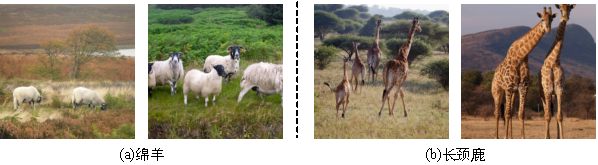
\includegraphics[width=\textwidth]{figs/shp2gir_coco.pdf}
  \caption{绵羊$\leftrightarrow$长颈鹿数据集示意图。图片来自文献\cite{lin2014microsoft}。}
  \label{fig:shp2gir_coco}
\end{figure}

\subsection{对比方法}

\textbf{CycleGAN}~作为非配对图像翻译的开山之作,Zhu等人\cite{zhu2017unpaired}提出的CycleGAN在多个数据集上取得令人信服的结果。

\textbf{U-GAT-IT}~Kim等人\cite{kim2019u}提出的U-GAT-IT引入一个注意力模块,通过基于辅助分类器得到的注意力图使模型更关注图像中可以区分两个域的区域,同时提出的自适应层实例归一化函数是利用在训练过程中从数据集中学到的参数在层归一化和实例归一化之间选择合适的比率。U-GAT-IT可以通过注意力机制和可学习的归一化函数使网络能够翻译需要整体变化或有较大形状变化的图像,因此与其对比。

\textbf{GANHopper}~Lira等人\cite{lira2020ganhopper}提出的GANHopper通过多个跳在两个域之间逐步翻译图像,网络不直接执行翻译,而是通过要求网络生成中间图像来控制翻译,这些中间图像类似于来自输入域图像之间的加权混合,但不对中间图像进行训练,所有跳都是用一个生成器沿着每个方向产生的,除此之外,还添加了一个平滑项来约束每个跳的大小。GANHopper在有形变的数据集(如狗转猫、人脸转猫脸)中可以实现翻译。

\textbf{InstaGAN}~Mo等人\cite{mo2018instagan}提出的InstaGAN利用实例分割图将目标分离,使每个目标有属于自己的实例分割图,将图像输入到图像编码器,此图像中每个目标的实例分割图逐个输入到实例编码器中,将得到的图像特征图与实例特征图按通道拼接并分别进入图像解码器和实例解码器得到生成图像和生成的实例分割图,生成的图像可以实现多目标形变图像翻译。

\subsection{评价指标}

$\mathbf{FID}$~Fr$\mathrm{\acute{e}}$chet Inception Distance(FID\cite{heusel2017gans})作为对现有的Inception Score(IS\cite{salimans2016improved})的改进而被提出。IS应用了效果优异的图像分类网络Inception v3,此网络可以对一组图像做分类预测,IS基于分类情况计算分数,但IS存在一个问题:仅考虑了生成图像的清晰度和多样性,而忽略了真实数据的影响。生成对抗网络的初衷是希望生成图像的分布尽量接近真实图像的分布,很显然,IS不能满足这一条件,因此FID应运而生,它可以更好地反映生成图像相较于真实图像的逼真度。

类似于IS,FID也使用了Inception v3模型,不同的是,FID并没有用Inception v3模型中最后一个用于分类的全连接层,而是提取了全连接层之前的2048维向量,因此每个图像被预测为2048个特征,可视为一个向量。对于真实图像,这个2048维向量是服从一个分布的,对于生成的图像,由它预测得到的向量也是一个分布,GAN的目标是使这两个分布尽量相同,问题此时转化为如何计算两个分布之间的距离。计算两个分布之间的距离,数学上可用Fr$\mathrm{\acute{e}}$chet距离或Wasserstein-2距离计算。

一个高斯分布可通过均值和方差确定,反过来说,如果给定两个相同的均值和方差,那么由这两个均值和方差确定的两个高斯分布相同,因此可以利用均值和方差来计算两个高斯分布之间的距离,两个分布之间的距离被定义为Fr$\mathrm{\acute{e}}$chet Inception Distance,即FID评价指标,可用公式表示为:
\begin{equation}
\begin{split}
FID(x,g)=\parallel\mu_x-\mu_g\parallel_2^2+Tr(\varSigma_x+\varSigma_g-2(\varSigma_x\varSigma_g)^{\frac{1}{2}})
\end{split}
\label{eq:FID}
\end{equation}
其中,$x$和$g$分别代表真实图像和生成图像,$\mu_x$和$\mu_g$表示的各自特征向量的均值,$\varSigma_x$和$\varSigma_g$为各自特征向量的协方差矩阵,$Tr$代表矩阵的迹(主对角线各元素的和)。FID的分数越低,即生成图像与真实图像之间的距离越小,代表生成图像的质量越好。

$\mathbf{LPIPS}$~Learned Perceptual Image Patch Similarity (LPIPS\cite{zhang2018perceptual})可用于衡量配对图像之间的相似程度。传统的图像相似度评价指标侧重于结构、内容等方面,优点为计算简单,但存在一个明显的缺点:与人的视觉感知存在较大差异,LPIPS指标的一大特点就是其得到的结果和人的视觉评价有更高的相关性。

假定有两幅图像$x$和$x_0$,利用一个预训练网络得到它们的深层特征,并计算出其特征之间的距离,从而得到$x$和$x_0$之间的相似性。为了评价生成结果的多样性,我们将从生成结果中随机采样,组成$n\times10$个图像对,其中$n$为数据集中图像的数量,然后计算每对图像之间的相似性,并将最终的平均值作为评价翻译结果多样性的LPIPS指标,LPIPS指标越大,代表翻译结果的内部多样性越好,反之越差。

\subsection{实验结果与分析}

\subsubsection{主观定性评价}

我们在绵羊$\leftrightarrow$长颈鹿数据集中实现两个方向的翻译,图\ref{fig:shp2gir}显示了绵羊转长颈鹿的定性结果,可以看出CycleGAN虽然可以生成长颈鹿的纹理且实现颈部拉长的效果,但不能生成一个完整的长颈鹿。U-GAT-IT对单个且清晰的绵羊可以实现翻译,但当绵羊的数量增多时,翻译无法完成,且与其它方法对比,其背景改动
\begin{figure}[ht]
    \centering
  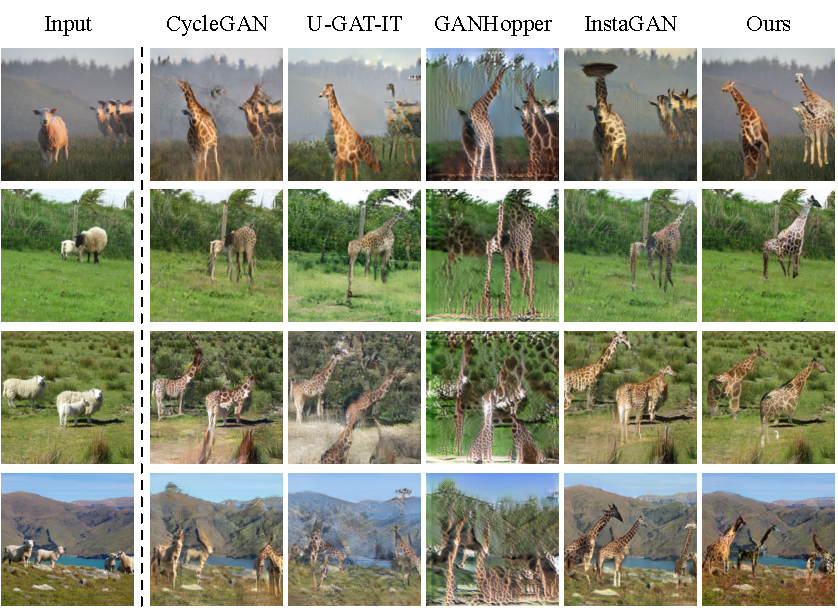
\includegraphics[width=\textwidth]{figs/shp2gir.pdf}
  \caption{绵羊转长颈鹿的定性结果图。}
  \label{fig:shp2gir}
\end{figure}
较大。GANHopper是这几种方法中效果最差的,整幅生成图像的目标和纹理都很混乱,InstaGAN可以部分实现绵羊至长颈鹿的翻译,但我们的方法相比较来说生成效果更好,多只绵羊都可以拥有长颈鹿的形状而不仅是纹理。


图\ref{fig:gir2shp}展示了长颈鹿转绵羊的定性结果,在此方向上的翻译效果整体比绵羊转长颈鹿的效果差一些,是因为数据集中大多数图像中的绵羊数量很多,目标物之间大多重叠且形态各异,给网络的学习增加了一定的难度。从图中可以看出,CycleGAN在形状上基本无变化,且纹理仍保留长颈鹿的纹理。U-GAT-IT的效果与CycleGAN类似,也无法实现翻译,但能看出其在形状上有一定的变化。GANHopper整体图像呈现模糊的效果,背景和前景目标都没有清楚的样式。InstaGAN和我们的方法在形状上都有变化,我们的方法可以实现每个目标都有更大程度的形变。

\begin{figure}[ht]
    \centering
  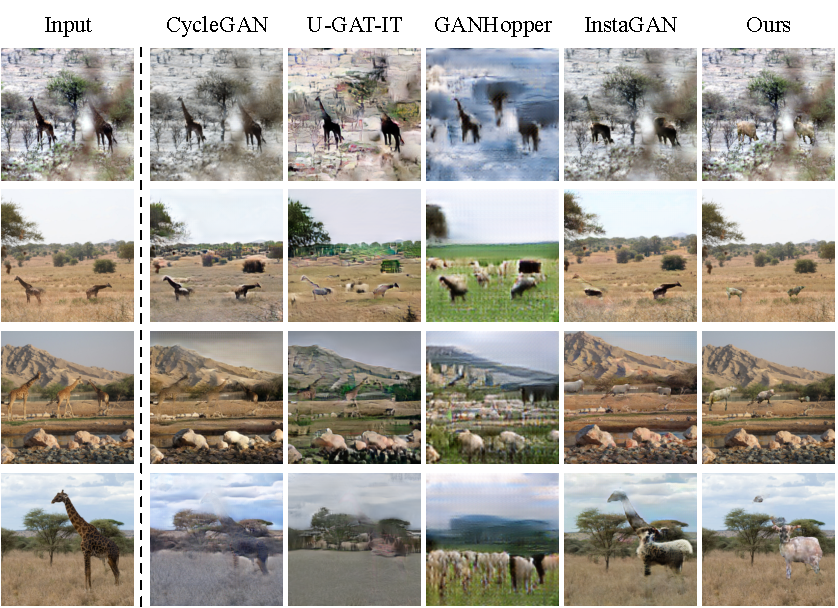
\includegraphics[width=\textwidth]{figs/gir2shp.pdf}
  \caption{长颈鹿转绵羊的定性结果图。}
  \label{fig:gir2shp}
\end{figure}

\subsubsection{客观定量评价}

绵羊转长颈鹿的定量结果和长颈鹿转绵羊的定量结果分别由表\ref{tab:shp2gir}和表\ref{tab:gir2shp}给出,FID指标评定生成图像的真实性,LPIPS指标评定生成图像的多样性。需注意的是:表中$\uparrow$代表此评价指标的值越大越好,反之$\downarrow$代表值越小越好;表中加粗的数字为最好的结果。从两个表中可以看出,GANHopper在绵羊$\leftrightarrow$长颈鹿两个任务上的FID分数都是最高的,说明它生成的结果与真实图像之间存在很大差异,这从图\ref{fig:shp2gir}和\ref{fig:gir2shp}中可以明显看出。除此之外,GANHopper在这两个任务上的LPIPS分数都是最低的,因为其生成的结果基本类似。CycleGAN在这两个任务上的FID和LPIPS指标优于GANHopper,但其生成结果还是存在一些失真,所以其FID指标在两个任务上都很低,但在长颈鹿转绵羊的任务上,结合\ref{fig:gir2shp}我们可以发现,CycleGAN并未完成翻译,生成图像和输入图像之间相差不大,所以这里LPIPS反映的是输入图像的多样性,因此分数较高。U-GAT-IT整体稍优于CycleGAN,但在两个任务上的LPIPS分数都偏低,说明其缺乏多样性。InstaGAN拥有较低的FID和较高的LPIPS分数,在绵羊转长颈鹿任务上,其FID分数与我们方法的FID分数接近,说明它真实性较好,但其LPIPS分数则显示在两个任务上与我们相差一定的多样性。本文提出的方法在绵羊转长颈鹿和长颈鹿转绵羊两个方向上都可以在获得较低FID分数的同时拥有较高的LPIPS分数,说明我们的方法生成的结果既有较高的真实性,也实现了域内的多样性,从而证明了我们方法的有效性。

\begin{table}[ht]
  \centering
  \caption{绵羊转长颈鹿的定量结果。}
    \begin{tabular}{c|c|c|c|c|c}
      \hline\noalign{\smallskip}
      方法 & CycleGAN & U-GAT-IT & GANHopper & InstaGAN & Ours \\
      \noalign{\smallskip}\hline\noalign{\smallskip}
      FID$\downarrow$   & 214.1329 & 212.0401 & 231.0558 & 192.8113 & \textbf{190.8434} \\
      LPIPS$\uparrow$ & 0.634$\pm$0.094 & 0.638$\pm$0.099 & 0.566$\pm$0.090 & 0.643$\pm$0.102 & \textbf{0.652$\pm$0.100} \\
    \noalign{\smallskip}\hline
    \end{tabular}
  \label{tab:shp2gir}
\end{table}

\begin{table}[ht]
  \centering
  \caption{长颈鹿转绵羊的定量结果。}
    \begin{tabular}{c|c|c|c|c|c}
      \hline\noalign{\smallskip}
      方法 & CycleGAN & U-GAT-IT & GANHopper & InstaGAN & Ours \\
      \noalign{\smallskip}\hline\noalign{\smallskip}
      FID$\downarrow$   & 242.0643 & 238.4553 & 276.8359 & 219.1365 & \textbf{211.4066} \\
      LPIPS$\uparrow$ & 0.662$\pm$0.100 & 0.658$\pm$0.106 & 0.608$\pm$0.103 & 0.665$\pm$0.102 & \textbf{0.673$\pm$0.102} \\
    \noalign{\smallskip}\hline
    \end{tabular}
  \label{tab:gir2shp}
\end{table}

\subsection{消融实验结果与分析}

因在多目标形变图像翻译中,形状和纹理的翻译效果对整个模型的性能起决定性作用,因此我们在形状翻译和纹理翻译阶段做消融实验。

\subsubsection{形状翻译}

为了探索不同结构的形状生成器$G_S$的作用,我们采用了三种结构组建形状生成器,第一种是下采样+上采样+跳连接,在下采样和上采样中分辨率相同的特征图之间添加跳连接,记作$G_S^{skip}$;第二种是下采样+残差块+上采样,其中残差块仅添加在下采样和上采样之间,记作$G_S^{res}$;第三种是下采样+残差块+上采样,其中残差块不仅添加在下采样与上采样之间,还添加在下采样和上采样中,共有5种尺度的残差块,记作$G_S^{multi\_res}$。

\begin{figure}[ht]
    \centering
  \includegraphics[width=.8\textwidth]{figs/ablation_study_shape.pdf}
  \caption{形状生成器采用不同结构的翻译结果示意图。}
  \label{fig:ablation_study_shape}
\end{figure}

从图\ref{fig:ablation_study_shape}可以看出,若采用$G_S^{skip}$结构,虽然会在形状上有所变化,但形状变化得不彻底,与长颈鹿的形状有一定差异,尤其是长颈鹿的头部区域,几乎没有头部的轮廓,而$G_S^{res}$可以较细致地生成长颈鹿的形状,头部和腿部生成得都较真实。这两种结构生成的图像存在差异的原因可能是在上采样过程中通过跳连接融合下采样时得到的各个尺度的特征图,使最终恢复的特征图融合了更多的低维特征,加强了输入图像对生成图像的限制能力,使生成图像不能最大限度地匹配真实样本的分布,去掉跳连接并加入残差块可解决此问题。图\ref{fig:ablation_study_shape}显示出相比较$G_S^{res}$,$G_S^{multi\_res}$可以生成更细致且逼真的结果,长颈鹿的轮廓边缘整体更流畅圆滑,且位置和身体的朝向更准确,推断产生这种结果的原因为$G_S^{res}$在单尺度上用残差块可能限制通过中间瓶颈的信息,从而限制网络的学习功能,而在上采样和下采样过程中加入残差块,使网络能够学习适用于较高和较低空间分辨率特征的多尺度转换,从而实现更彻底的形状翻译。

\subsubsection{纹理翻译}

不同结构的纹理生成器$G_T$对纹理翻译结果的影响也是我们研究的重点,纹理生成得越细致,整体图像越逼真,我们采用下采样+残差块+上采样(记作$G_T^{res}$)和下采样+上采样+跳连接(记作$G_T^{skip}$)两种结构生成纹理,除此之外,还探讨了在这两种结构的基础上加入颜色损失对纹理翻译效果的影响,分别记作$G_T^{res}$+color和$G_T^{skip}$+color。

\begin{figure}[ht]
    \centering
  \includegraphics[width=\textwidth]{figs/ablation_study_texture.pdf}
  \caption{纹理生成器采用不同结构,并分别加入颜色损失的翻译结果示意图。}
  \label{fig:ablation_study_texture}
\end{figure}

从图\ref{fig:ablation_study_texture}整体看,采用跳连接的生成效果更佳,与形状翻译不同,在此过程中,我们希望生成的纹理与输入图像所对应的纹理尽量一致,跳连接可以保证网络在翻译过程中融合并学习更多的特征信息,加入的颜色损失可进一步优化纹理的生成效果,使边缘生成得更清楚。从图\ref{fig:ablation_study_texture}可以明显看出纹理生成效果最优的为$G_T^{skip}$+color,纹理较清晰细致,且没有彩色的亮斑,因此我们的纹理生成器采用$G_T^{skip}$结构,并引入颜色损失。

\section{讨论}

从前面的实验分析中可以看出,尽管我们的方法在多目标形变图像翻译任务上可以取得比其它方法更佳的结果,但整体生成效果仍存在提升空间。目前大多数做形变翻译的工作集中于单目标形变图像翻译,输入图像无背景、目标明显,两个域的目标之间差异度较低,如狗与猫、人脸与漫画脸、人脸与猫脸等,而绵羊与长颈鹿的差异度相比较更高一些,且图像中存在多个目标,这导致多目标形变图像翻译具有极大的挑战性。我们的方法利用实例分割图获取每个目标的实例信息,并将复杂的问题分为几个小问题逐个解决,虽可以实现翻译,但当多个目标存在重叠时,目前的方法还不能实现准确地逐个翻译,所以这个问题还有待研究。

\section{本章小结}

本章介绍了多目标形变图像翻译问题,并为解决此问题提出我们基于生成对抗网络的模型。

在第一节中,我们简要介绍了形变翻译与侧重纹理翻译任务的区别,并进一步介绍了多目标形变图像翻译任务。

在第二节中,我们确定了多目标形变图像翻译需要考虑两个问题,且在探索过程中发现实例分割图更易于完成形状翻译,因此提出了一个模型,将形状、纹理和背景分开处理,融合细化后得到最终的生成图像,还介绍了各部分的网络结构及其对应的目标函数。

在第三节中,我们介绍了实验用到的数据集、对比方法和评价指标,并从定性和定量两方面分析实验结果,对形状翻译和纹理翻译部分的生成器结构和损失做了相应的消融实验,从实验显示的结果确定最优的方案。

在最后一节中,我们讨论了本方法存在的一些局限性,并指出需要改进的地方,确定了今后的研究方向。


\chapter{基于生成对抗网络的水下图像翻译}

\section{引言}

近年来,随着全球资源的日益短缺以及社会发展所产生的对资源的迫切需求,占据全球表面积71$\%$的海洋逐渐进入人们的视线。海洋中蕴含着丰富的资源,如果能够利用海洋资源,将缓解当下资源短缺的情况。目前,开发、研究和勘探海洋资源已成为国际社会关注的焦点。当研究水下环境时,清晰的水下图像和视频可以提供更有价值的信息,对于水下考古、水下勘探和水下开采等许多工作至关重要,然而原始的水下图像和视频通常受到水下环境中吸收、散射等影响,造成图像出现模糊、对比度低、雾状等效果,整体呈现蓝色调或绿色调,严重阻碍水下研究的进行。

提升水下图像的可视质量,解决雾化、模糊、色偏等问题的任务可视为水下图像清晰化,之前的传统工作可根据是否基于物理模型划分:基于非物理模型的方法是修改图像像素值以提高视觉质量,不需要考虑水下图像的成像原理和退质过程;基于物理模型的方法是从给定图像中估计成像模型的潜在参数。随着深度学习在低级视觉问题上取得的显著进展,数据驱动的方法越来越引起人们的关注,基于深度学习的方法根据其采用的主要模型可分为基于卷积神经网络的方法和基于生成对抗网络的方法。基于卷积神经网络的方法忠于原始的水下图像,基于生成对抗网络的方法旨在提高图像的感知质量,因基于生成对抗网络的方法更适于由多种因素导致的图像退化,因此本节设计的网络架构基于生成对抗网络。与第二章介绍的图像翻译相联系,水下图像清晰化也可看作一个图像翻译任务:给定一张水下退质图像,目的是生成一张高质量的去雾去噪、无色偏且高对比度的图像,本节利用第二章中介绍的分解表示实现非配对数据集情况下的水下图像清晰化。

\section{水的光学特性}

我们透过清澈的水观察水底的生物时,以为看到的场景与在空气中看到的一致,殊不知即使是这种清澈的水质,光在其中也存在严重的衰减,这一衰减主要是由吸收和散射引起的。水中的粒子吸收大部分光能量,导致颜色偏蓝绿色调,而散射过程包括光与水中颗粒(如沙子和浮游生物等)碰撞后的一系列方向变化,会对水下成像产生类似于雾天对室外视野的影响。

由于光衰减的波长相关性,水对光的吸收具有明显的选择性,图\ref{wavelength}显示出不同波长的光在水中的传播距离,红色光在4-5米后迅速消失,橙色光大多在5米深度处消失,黄色光在10米深度处完全消失,绿色光在20米深度处消失,且绿色波长在沿海水域传播得更远,蓝色则可以达到在水中传播50米深度以上才消失,在海洋中传播得更好。因此,水下图像颜色通常以偏蓝色或偏绿色为主(如图\ref{color}(a)所示),给水下中远距离的拍摄增加困难,一些有价值的信息会因吸收而丢失。

\begin{figure}[ht]
    \centering
	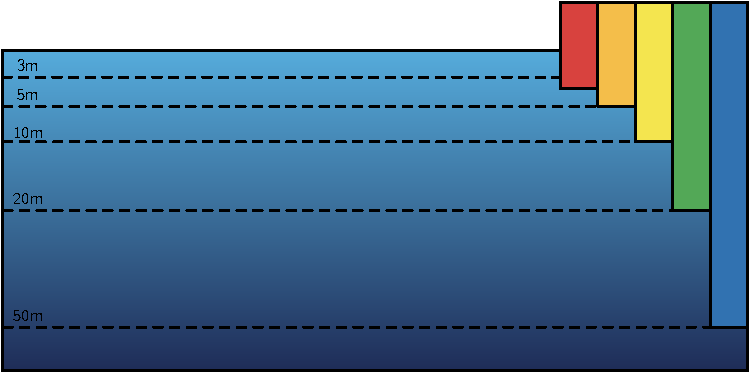
\includegraphics[width=\textwidth]{figs/wavelength.pdf}
	\caption{不同波长在水中的传播距离。图片来自文献\cite{han2018review}。}
	\label{wavelength}
\end{figure}

如果水对光仅存在吸收作用,那么可以通过增设人工光源来增加水下拍摄距离,但水对光还存在散射特性,随着人工光源的增强,散射作用愈见强烈。当我们用照相机拍摄水下场景时,根据Jaffe-McGlamery水下成像模型\cite{jaffe1990computer}\cite{mcglamery1980computer},由照相机拍摄的水下图像可以表示为以下分量的和:(1)直接分量$D$:场景中物体表面的反射光在传播过程中没有被散射的部分;(2)前向散射分量$F$:场景中物体表面的反射光在传播过程中发生小角度散射的部分;(3)后向散射分量$B$:介质中的粒子将入射到它们身上的光散射到许多其它方向,后向散射是这些光子到达照相机而形成的信号,不携带有关场景的信息。文献\cite{schechner2004clear}已经证明了$F\ll D$,前向散射对图像退化没有明显影响,所以仅考虑直接分量和后向散射分量,其中后向散射分量是导致水下图像质量下降的主要原因,会降低对比度,在水下图像中产生模糊和雾状效果(如图\ref{color}(b)所示)。

\begin{figure}[htp]
    \centering
	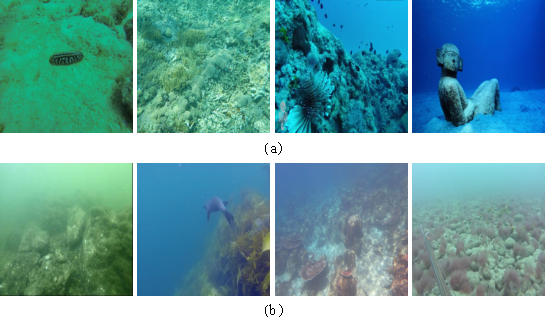
\includegraphics[width=\textwidth]{figs/color.pdf}
	\caption{(a)因水对光的选择吸收特性导致呈现蓝色调或绿色调的水下图像, (b)因水对光的散射特性而产生模糊和雾状效果的水下图像。图片来自文献\cite{fabbri2018enhancing}\cite{islam2019fast}。}
	\label{color}
\end{figure}

\section{模型算法}

现有两个域:水下图像域和清晰图像域,水下图像整体呈蓝绿色调且多显模糊,有雾状效果,而清晰图像可以看出图像中所有对象原本的颜色,对比度高且清晰度高。本节提出一个基于分解表示的框架,用于在无配对数据集情况下将水下图像域中的图像翻译到清晰图像域中。本节提出将图像分解到两个空间,具体来说,水下图像分解为:(1)色彩空间,其中含有吸收导致的水下图像特有的蓝绿色调;(2)信息空间,其包含了损失部分信息的内容和额外的雾、噪声等,清晰图像分解为:(1)色彩空间,其中包含对象和场景的真实色调;(2)信息空间,其中的信息丰富,拥有很多水下图像域没有的细节信息。

我们发现之前的基于分解表示的图像翻译方法虽然可以做到部分的颜色变化,但并不能保证水下图像中有用信息的完整性并添加来自清晰图像的信息(如图\ref{examples}),其翻译效果并不理想,为了解决这个问题,本节提出两个网络:特征提取网络和映射网络。特征提取网络在残差网络的基础上进行修改,旨在对映射到清晰图像域信息空间中的特征做进一步的特征提取和融合,尽可能多地学习清晰图像的信息。映射网络用于学习从水下图像域信息空间到清晰图像域信息空间的映射,在潜在空间中做映射是因为在紧凑的低维潜在空间中的映射原则上比在高维图像空间中更容易学习。通过我们提出的网络框架,可以在不同水下数据集上进行水下图像清晰化。

\begin{figure}[ht]
    \centering
	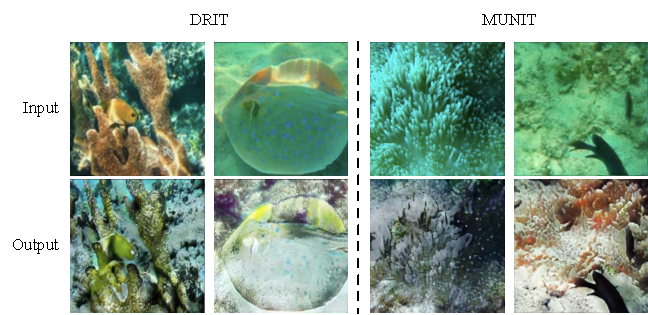
\includegraphics[width=\textwidth]{figs/DRIT_MUNIT_train_examples.pdf}
	\caption{DRIT和MUNIT在水下数据集上做图像翻译的效果。}
	\label{examples}
\end{figure}

\subsection{算法框架}

我们的目标是在无配对数据集的情况下,实现水下图像域$X$中的图像$x\in X$到清晰图像域$Y$中的图像$y\in Y$的翻译,如图\ref{architecture_underwater}所示,我们的框架包括色彩编码器$\{E_X^H, E_Y^H\}$,信息编码器$\{E_X^I, E_Y^I\}$,生成器$\{G_X, G_Y\}$,映射网络$M$和特征提取网络$FE$。在$X\rightarrow Y$方向上,图像$x$经过色彩编码器$E_X^H$得水下图像的色彩特征$h_x=E_X^H(x)$,同时$x$经信息编码器$E_X^I$得水下图像的信息特征$i_x=E_X^I(x)$,类似地,图像$y$经色彩编码器$E_Y^H$得清晰图像的色彩特征$h_y=E_Y^H(y)$,经信息编码器$E_Y^I$得清晰图像的信息特征$i_y=E_Y^I(y)$。如果按照DRIT和MUNIT的方式,那么将简单地把$i_x$和$h_y$输入到$G_B$中,以得到生成的清晰域图像$\hat{y}=G_B(i_x, h_y)$,由图\ref{examples}展示的DRIT和MUNIT翻译结果,我们推断水下图像的信息特征可能不足,不能与清晰图像的色彩信息一起生成清晰的图像,在生成清晰图像前,最好将水下图像的信息特征与清晰图像的信息空间对齐,且清晰图像的信息特征包含的信息越多越好。基于此推断,我们提出:(1)对清晰域的信息做进一步特征提取的特征提取网络$FE$,即$i_y^{fe}=FE(i_y)$,使其可以学习局部密集的信息特征,包含更多的细节信息;(2)将水下图像的信息特征$i_x$映射到清晰图像的信息空间中的映射网络$M$,即$i_x^m=M(i_x)$,使信息特征$i_x^m$与$Y$域的信息空间对齐,需要注意的是,此时应与经过特征提取的信息空间对齐。然后将$i_x^m$和$h_y$输入到生成器$G_Y$中,得到生成的清晰图像$\hat{y}=G_Y(i_x^m, h_y)$,综合上述,可以得到完整的由水下图像翻译到清晰图像的过程:
\begin{equation}
\begin{split}
\hat{y}=G_Y(i_x^m, h_y)=G_Y(M(i_x), h_y)=G_Y(M(E_X^I(x)), E_Y^H(y))
\end{split}
\label{eq:underwater_X2Y}
\end{equation}
由$X\to Y$可以类比出$Y\to X$方向上的翻译过程:
\begin{equation}
\begin{split}
\hat{x}=G_X(i_y^{fe}, h_x)=G_X(FE(i_y), h_x)=G_X(FE(E_Y^I(y)), E_X^H(x))
\end{split}
\label{eq:underwater_X2Y}
\end{equation}

\begin{figure}[ht]
    \centering
	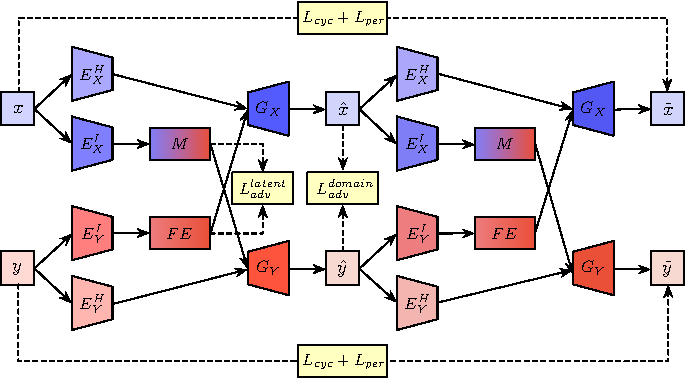
\includegraphics[width=\textwidth]{figs/architecture_underwater.pdf}
	\caption{水下图像清晰化模型示意图。}
	\label{architecture_underwater}
\end{figure}

\subsection{特征提取网络}

如图\ref{FE}所示,特征提取网络$FE$由9个特征提取网络块$FEB$组成,受ResNet\cite{he2016deep}和DenseNet\cite{huang2017densely}的启发,每个特征提取网络块$FEB$包括两组结构:一组包含卷积层$Conv$、实例归一化层$IN$\cite{ulyanov2016instance}和非线性激活函数$ReLU$\cite{nair2010rectified},一组包含卷积层$Conv$和实例归一化层$IN$,和ResNet不同的是,输入不仅与$FEB$的输出相加,还与第一组结构的输出按通道拼接,这样将残差块和密集连接整合到一起,既保留了残差块利用之前的特征的特点,又加入密集连接以渲染更多细节,从而达到对清晰图像的细节特征充分学习和整合的目的。经过9个$FEB$的顺序处理后,再将$FE$的输入与$FE$的输出相加,构成一个大的残差块,再次利用之前的特征。

\begin{figure}[ht]
    \centering
	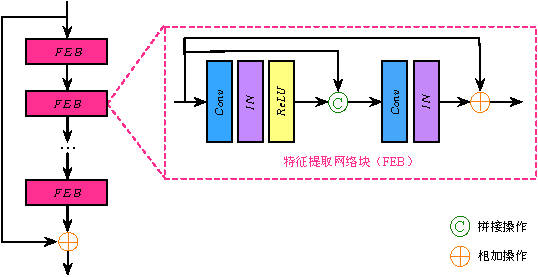
\includegraphics[width=\textwidth]{figs/FE.pdf}
	\caption{特征提取网络的网络结构示意图。}
	\label{FE}
\end{figure}

\subsection{映射网络}

映射网络将水下图像的信息特征映射到清晰图像的信息空间,需要做的是去掉水下图像中与雾、模糊等相关的信息,与清晰图像的信息空间对齐。针对去掉雾等信息,我们引入图像去雾相关操作,主要采用的是去雾文献\cite{hong2020distilling}提出的空间加权残差通道注意块$SWRCAB$,之前的去雾模块用全局平均池化操作来学习每个通道的权重,该权重将所有输入特征聚合并取平均,会忽略在不同通道上雾的浓度不同的问题,$SWRCAB$通过学习内容感知通道注意力以对严重退化的区域和信息通道施以更多关注,其首先用卷积层和非线性激活函数$Sigmoid$学习输入特征的空间权重,然后通过逐元素相乘的操作得到有空间权重的特征,最后通过一个全局池化层、全连接层和非线性激活函数$Sigmoid$来得到每个通道的注意力。类似于特征提取网络,由3个$SWRCABS$组成一个残差块,记作$RIR$,又用6个$RIR$构成最终的映射网络。

我们方法的关键之处在于使水下图像的信息特征可以映射到清晰图像的信息空间中,受之前的工作\cite{lee2018diverse}\cite{wan2020bringing}的影响,我们在此处用对抗损失来缩小两个域的信息空间之间的域差距,具体来说,我们训练一个潜在空间判别器$D^{L}$来判别$i_x^m$和$i_y^{fe}$,这个对抗损失可表示为:
\begin{equation}
\begin{split}
\mathcal{L}_{adv}^{latent} & = \mathbb{E}_x[\frac{1}{2}\log D^{L}(M(E_X^I(x))) + \frac{1}{2}\log(1-D^L(M(E_X^I(x))))] \\
& + \mathbb{E}_y[\frac{1}{2}\log D^{L}(FE(E_Y^I(y))) + \frac{1}{2}\log(1-D^L(FE(E_Y^I(y))))]
\end{split}
\label{eq:latent_GAN}
\end{equation}

\subsection{目标函数}

\subsubsection{循环一致性损失}

因为整个网络是在无配对图像的条件下训练的,所以借鉴CycleGAN\cite{zhu2017unpaired}的循环一致性损失来限制生成图像,以此弥补无配对数据集的缺陷。当给定$x\in X$和$y\in Y$,利用信息编码器和色彩编码器将其分别编码为$\{i_x, i_y\}$和$\{h_x, h_y\}$,再通过映射函数和特征提取函数分别将$i_x$和$i_y$编码为$i_x^m$和$i_y^{fe}$,通过交换两个域此时的信息特征和色彩特征,得到跨域生成图像$\{\hat{x}, \hat{y}\}$。为了实现循环,将$\{\hat{x}, \hat{y}\}$进行再分解,利用信息编码器和色彩编码器将$\{\hat{x}, \hat{y}\}$分别编码为$\{\hat{i}_x, \hat{i}_y\}$和$\{\hat{h}_x, \hat{h}_y\}$,然后$\hat{i}_x$经过映射函数得到$\hat{i}_x^m$,$\hat{i}_y$经特征提取函数得$\hat{i}_y^{fe}$,再次将两个域此时的信息特征和色彩特征进行交换,得到循环重建后的图像,即:
\begin{equation}
\begin{split}
\tilde{x}=G_X(\hat{i}_y^{fe}, \hat{h}_x) & =G_X(FE(\hat{i}_y), \hat{h}_x)=G_X(FE(E_Y^I(\hat{y})), E_X^H(\hat{x})) \\
\tilde{y}=G_Y(\hat{i}_x^{m}, \hat{h}_y) & =G_Y(M(\hat{i}_x), \hat{h}_y)=G_Y(M(E_X^I(\hat{x})), E_Y^H(\hat{y}))
\end{split}
\label{eq:cycle}
\end{equation}
经过两次跨域翻译后,生成的图像$\{\tilde{x}, \tilde{y}\}$应可以重建原始图像$\{x, y\}$(如图\ref{architecture_underwater}所示),为了对此进行约束,在此引入循环一致性损失:
\begin{equation}
\begin{split}
\mathcal{L}_{cyc}=\mathbb{E}_x[\parallel\tilde{x}-x\parallel_1] + \mathbb{E}_y[\parallel\tilde{y}-y\parallel_1]
\end{split}
\label{eq:cycle_consistenty}
\end{equation}

\subsubsection{感知损失}

感知损失利用预先训练好的VGG网络分别提取生成图像和真实图像的特征,并尽量使二者的特征相似,从而使生成图像和真实图像的高层信息相接近,避免计算像素级误差的损失无法捕捉感知区域的问题。在本节中,比较输入图像和循环重建图像之间的感知损失:
\begin{equation}
\begin{split}
\mathcal{L}_{per}=\mathbb{E}_{x,y}\sum_{i=1}^T\frac{1}{N_i}[\parallel\Phi_{VGG}^i(\tilde{x})-\Phi_{VGG}^i(x)\parallel_1 + \parallel\Phi_{VGG}^i(\tilde{y})-\Phi_{VGG}^i(y)\parallel_1]
\end{split}
\label{eq:perceptual}
\end{equation}
其中$T$代表总层数,$N_i$代表每一层元素的数量,$\Phi_{VGG}^i$代表VGG网络的第$i$层特征图。

\subsubsection{域对抗损失}

类似于DRIT\cite{lee2018diverse},我们引入域对抗判别器$\{D_X, D_Y\}$以判别每个域的真实图像与生成图像,在判别的过程中,$\{G_X, G_Y\}$致力于生成能够以假乱真的图像去欺骗域判别器,域对抗损失定义为:
\begin{equation}
\begin{split}
\mathcal{L}_{GAN}^{domain}& = \mathbb{E}_x[\log D_X(x)] + \mathbb{E}_x[\log(1-D_X(\hat{x}))] \\
& + \mathbb{E}_y[\log D_Y(y)] + \mathbb{E}_y[\log(1-D_Y(\hat{y}))]
\end{split}
\label{eq:GAN_loss}
\end{equation}

\subsubsection{KL损失}

我们在信息编码和色彩编码上应用KL散度来惩罚高斯先验和这些潜在分布的偏差,具体定义为:
\begin{equation}
\begin{split}
\mathcal{L}_{KL}& = \mathnormal{KL}(E_X^I(i_x|x)\parallel \mathcal{N}(0,1)) + \mathnormal{KL}(E_X^H(h_x|x)\parallel \mathcal{N}(0,1)) \\
 & + \mathnormal{KL}(E_Y^I(i_y|y)\parallel \mathcal{N}(0,1)) + \mathnormal{KL}(E_Y^H(h_y|y)\parallel \mathcal{N}(0,1)) \\
 & + \mathnormal{KL}(M(i_x^m|i_x)\parallel \mathcal{N}(0,1)) + \mathnormal{KL}(FE(i_y^{fe}|i_y)\parallel \mathcal{N}(0,1))
\end{split}
\label{eq:KL}
\end{equation}

\subsubsection{自重建损失}

为了保证分解得到的信息编码和色彩编码的完整性,类似于DRIT\cite{lee2018diverse},我们使由一幅图像分解得到的信息编码和色彩编码再经生成器,生成和原始输入尽量一致的图像,即$G_X(i_x, h_x)\approx x$,因此加入自重建损失,定义为:
\begin{equation}
\begin{split}
\mathcal{L}_{scyc}=\mathbb{E}_x[\parallel G_X(i_x, h_x)-x\parallel_1] + \mathbb{E}_y[\parallel G_Y(i_y, h_y)-y\parallel_1]
\end{split}
\label{eq:self_cyc}
\end{equation}

\subsubsection{总损失函数}

综合上述所描述的损失函数,得到最终的目标函数为:
\begin{equation}
\begin{split}
\min \limits_{G, E^I, E^H, M, FE} \max \limits_{D, D^L} \mathcal{L}_{total} 
& = \lambda_{adv}^{domain}\mathcal{L}_{adv}^{domain} + \lambda_{adv}^{latent}\mathcal{L}_{adv}^{latent}+ \lambda_{cyc}\mathcal{L}_{cyc} \\
& + \lambda_{per}\mathcal{L}_{per} + \lambda_{KL}\mathcal{L}_{KL} + \lambda_{scyc}\mathcal{L}_{scyc}
\end{split}
\label{eq:total}
\end{equation}
其中$\lambda_{adv}^{domain}$、$\lambda_{adv}^{latent}$、$\lambda_{cyc}$、$\lambda_{per}$、$\lambda_{KL}$和$\lambda_{scyc}$是超参数,用于控制和协调各项损失函数的权重以平衡损失。

\subsection{模型部署}

% 此处的引用看超哥的43页
\textbf{网络架构}~信息编码器和色彩编码器都由卷积神经网络构成,并加入$ReLU$激活函数\cite{nair2010rectified}和实例归一化\cite{ulyanov2016instance},采用实例归一化是因为水下图像数据集的场景多且杂,每个样本包含的独特信息都需要学习。生成器由残差块和转置卷积层构成,同样在每一层加入$ReLU$激活函数和实例归一化,除了最后一层用激活函数$Tanh$。判别器有两种,一种是简单的由堆叠卷积层构成的网络,用作对潜在空间进行判别,另一个采用多尺度判别器\cite{wang2018high},用于更好地学习整体轮廓和具体细节。

\textbf{训练细节}~整个网络基于PyTorch框架在256$\times$256分辨率的图像上训练,采用Adam\cite{kingma2014adam}优化算法并将批大小设为1,对于超参数,我们设置$\lambda_{adv}^{domain}=\lambda_{adv}^{latent}=1$,$\lambda_{cyc}=\lambda_{per}=\lambda_{scyc}=10$,$\lambda_{KL}=0.1$。

\section{实验}

\subsection{数据集设置}

$\mathbf{EUVP}$~由Islam等人\cite{islam2019fast}提出,包含大量感知质量高和感知质量低的配对和非配对水下图像,这些图像是在不同能见度、不同地点下进行的海洋探测和人机协同实验中收集的,除此之外,还包含一些从公开的YouTube视频中提取的图像,数据集中的图像包含不同的场景、水体类型和照明条件等,以适应广泛的自然变化。利用CycleGAN在由失真和未失真的水下图像构成的非配对数据集上训练,生成的失真图像和真实的未失真图像构成EUVP的配对数据集。配对数据集根据图像中的内容分为“Underwater Dark”(共5550对)、“Underwater ImageNet”(共3700对)和“Underwater Scenes”(共1364对),并提供一个可用于测试的“test samples”(共515对)。非配对数据集的获得则相对简单些,由6个志愿者根据其视觉感知效果的优劣分为两组,其中质量高的有3140张图像,质量低的有3195张图像。为了满足我们的训练需求,我们从非配对数据集中根据颜色、对比度和清晰度等图像属性进一步挑选,挑选的宗旨是:视觉感知效果好的域应仅包含清晰度和对比度高、没有色偏和雾状效果,同时包含尽量多的场景;视觉感知效果差的域应包含不同场景、不同浑浊度、不同颜色和不同照明条件的图像。最终,我们选出视觉效果优劣的图像分别为1310张和1295张用于训练(如图\ref{train}),分别用“test samples”中的配对图像和非配对图像中的“validation”做配对和非配对的测试。

\begin{figure}[ht]
    \centering
	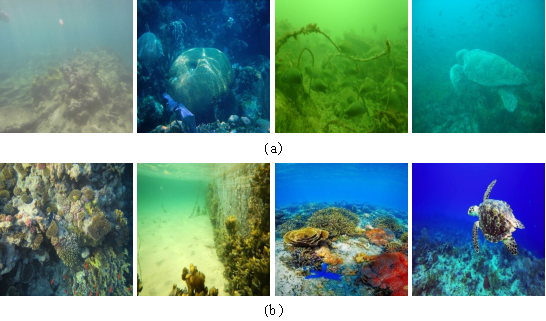
\includegraphics[width=\textwidth]{figs/train.pdf}
	\caption{(a)失真程度小、视觉效果好的水下图像, (b)失真程度大且视觉效果低的水下图像。图片来自文献\cite{islam2019fast}。}
	\label{train}
\end{figure}

$\mathbf{UIEB}$~由于缺乏充足且有效的训练数据,基于深度学习的水下图像增强方法的性能受到限制,由Li等人\cite{li2019underwater}提出的UIEB数据集提供了大量配对水下图像。Li等人从Google、YouTube和其它相关文献中收集图像,经过挑选,大多数图像被丢弃,剩下950张图像,对选出的图像分别用9种水下图像增强方法、2种图像去雾方法和1个水下图像增强的商业应用处理,每张图像都有对应的12张增强图像,找50个志愿者为每一个水下图像选择一个参考图像。若选择的参考图像中有超过半数的票被记为不满意,则其对应的原始水下图像视为具有挑战性的图像,并且将该图像的参考图像丢弃。由此共得到890对配对图像以及60张有挑战性的水下图像。之前的水下图像增强方法在评估的时候主要是使用合成的数据集或少数真实图像,UIEB数据集提供的参考图像数量大,颜色相对真实且可见性和亮度明显改善,在评估的时候更有说服力,因此将UIEB用作测试集。

$\mathbf{SUN}$~由Xiao等人\cite{xiao2016sun}提出的SUN数据集包含908个类别和131067张图像,本节仅关注此数据集中的水下图像,包含的场景有珊瑚礁、海洋深层、海洋浅层、水池和沉船,共713张图像,可用作测试集。

$\mathbf{RUIE}$~由Liu等人\cite{liu2019real}提出的RUIE数据集分为3个子集:水下图像质量子集(UIQS)、水下色偏子集(UCCS)和水下高级任务驱动子集(UHTS)。水下图像质量子集用UCIQE评价指标对这些图像打分,并按照所得分数排序,将其分为5类:A、B、C、D和E,每种水类型都有726张图像;水下色偏子集根据CIElab颜色空间中蓝色通道(红色-绿色偏差)的平均值生成,包含蓝色、蓝绿色和绿色三种颜色类型,每种类型都有100张图像;水下高级任务驱动子集包含集中海洋生物,目的是评估水下图像增强算法对高级计算机视觉任务(如分类和检测)的影响,为了探讨图像质量对检测精度的影响,将UHTS分为5个子集,每个子集包含60张图像。本节用UIQS测试不同算法在不同水条件下的性能,用UCCS评估不同算法校正色偏的能力。

\subsection{对比方法}

因本节将图像翻译应用到水下图像清晰化,所以不仅和图像翻译方法对比,也与几种水下图像增强方法对比。

\subsubsection{水下图像增强方法}

$\mathbf{UWCNN}$~Li等人\cite{li2020underwater}于2020年提出一种基于水下场景先验的水下图像增强卷积神经网络模型,称为UWCNN,此模型无需估计水下成像模型的参数,而是直接重建清晰的潜在水下图像。UWCNN的成功得益于其提出的水下合成数据集,因为基于深度学习的方法若缺乏充足有效的训练数据会限制模型的性能,因此Li等人在NYU-v2室内数据集\cite{silberman2012indoor}上根据水下成像物理模型和水下场景光学特性提出一个水下图像合成算法,可以模拟多种不同的水类型和降解水平。UWCNN可以在此数据集上训练以增强每种合成的水下场景类型,并推广到真实的水下图像中。

$\mathbf{UIE}$-$\mathbf{DAL}$~Uplavikar等人\cite{uplavikar2019all}认为水下图像因吸收和散射而呈现不同的水质,利用一个模型就可以对各种水质实现水下图像增强是极具挑战性的,UIE-DAL引入额外的妨害分类器消除不同水质对水下图像内容学习的干扰,从而很好地处理增强过程中水的多样性。模型在UWCNN合成水下数据集上训练,训练好的模型可泛化于真实水下图像。

$\mathbf{Deep~SESR}$~Islam等人\cite{islam2020simultaneous}提出的Deep SESR结合了密集残差子网,利用可解决特定水下颜色退化、图像清晰度不足和高级特征表示的多模态目标函数进行监督学习,辅以可指导网络学习全局对比度增强的前景区域(数据集提供),可同时处理水下图像增强和超分辨率的问题。因本节不进行超分辨性能的对比,所以仅利用其增强结果。

$\mathbf{Water}$-$\mathbf{Net}$~由fusion-based\cite{ancuti2012enhancing}得到启示,Li等人\cite{li2019underwater}采用多个预处理操作和融合策略,根据水下图像退化的特点,分别采用白平衡(WB)、直方图均衡化(HE)和Gamma校正(GC)算法处理原始水下图像以生成三个输入,将原始水下图像和处理后的三个输入图像输进提出的卷积神经网络Water-Net中,由公式\ref{eq:UIEB}可以看出最终得到的增强图像是三者融合,白平衡用于校正色偏,直方图均衡化和Gamma校正则用于提高对比度,提高黑暗区域的亮度。
\begin{equation}
\begin{split}
I_{en}=R_{WB}\odot C_{WB}+R_{HE}\odot C_{HE}+R_{GC}\odot C_{GC}
\end{split}
\label{eq:UIEB}
\end{equation}
其中$I_{en}$是增强结果,$\odot$代表矩阵的逐元素相乘,$R_{WB}$、$R_{HE}$和$R_{GC}$分别为原始水下图像经过WB、HE和GC处理后的结果,$C_{WB}$、$C_{HE}$和$C_{GC}$则为网络学到的置信图。

$\mathbf{UGAN}$~Islam等人\cite{fabbri2018enhancing}利用CycleGAN在挑选出的非配对失真和未失真水下图像上训练,将未失真图像和生成的失真图像配对,UGAN利用生成对抗网络在配对数据集上训练以增强水下图像。

\subsubsection{图像翻译方法}

$\mathbf{CycleGAN}$~Zhu等人\cite{zhu2017unpaired}提出的CycleGAN是非配对图像翻译的开山之作,在多个数据集上都有优异的表现,因此我们将其应用于水下图像转清晰图像的应用中。

$\mathbf{MSGAN}$~Mao等人\cite{mao2019mode}提出的MSGAN提出一个可以应用到多个框架的通用正则化项,在非配对图像翻译任务中,MSGAN以DRIT为基础框架,可以得到比DRIT更多样、更清晰的图像,因此我们在此不与DRIT对比,而是与效果更好的MSGAN对比。

$\mathbf{DSMAP}$~Chang等人\cite{chang2020domain}提出的DSMAP相比较MUNIT和DRIT做了进一步映射,我们提出的框架也是在DRIT和MUNIT的基础上进一步映射,虽都是再映射,但映射的方式不同,因此我们与DSMAP做对比以比较在水下图像清晰化任务上更有效的映射方式和网络框架。

\subsection{评价指标}

在生成水下图像时,不同的模型可能会产生不同的效果,存在不同程度的失真,进而导致视觉效果的降低。本节会提供在每个数据集上每个算法的视觉效果图,除此之外,为了在量化视觉图像质量,本节还会提供能够自动预测感知图像质量的定量指标。对水下图像质量的评估可根据是否需要参考图像分为有参考图像评价指标和无参考图像评价指标,常用的有参考图像评价指标有:SSIM\cite{wang2004image}、PSNR、MSE等,常用的无参考图像评价指标有UCIQE\cite{yang2015underwater}和UIQM\cite{panetta2015human}。

$\mathbf{MSE}$~均方误差(Mean Square Error)旨在提供代表两个信号之间相似性或失真的定量评分,通常情况下,一个信号是原始信号,另一个信号是从某种失真中恢复的,从数学上讲,两个信号之间的MSE可以表示为:
\begin{equation}
\begin{split}
MSE = \frac{1}{N}\sum_{i=1}^{N}(x_i - y_i)^2
\end{split}
\label{eq:example}
\end{equation}
其中$x$和$y$为两个信号,$x_i$和$y_i$是在位置$i$的像素,$N$是像素数量。MSE得分较低的结果表明其在图像内容方面更接近参考图像。

$\mathbf{PSNR}$~峰值信噪比(Peak Signal to Noise Ratio)在MSE的基础上再做一步处理,可用公式表示为:
\begin{equation}
\begin{split}
PSNR = 10\log_{10}\frac{L^2}{MSE}
\end{split}
\label{eq:example}
\end{equation}
其中$L$代表图像像素强度的动态范围(图像为255),PSNR得分较高的结果表明其在图像内容方面更接近参考图像。

$\mathbf{SSIM}$~结构相似性(Structural SIMilarity)由Wang等人\cite{wang2004image}提出,相比较MSE和PSNR侧重于内容的完整性与相似性,SSIM主要计算生成图像与真实图像之间的结构相似性。每幅图像都有其自己特定的结构,表现为图像的像素之间存在相关性,SSIM从此角度出发,比较生成图像与参考图像之间的亮度、对比度和局部结构。考虑从两个相比较图像的相同位置获取的局部区域块$x$和$y$,可将亮度$l(x,y)$、对比度$c(x,y)$和局部结构$s(x,y)$相乘得SSIM分数:
\begin{equation}
\begin{split}
SSIM=l(x,y)\cdot c(x,y)\cdot s(x,y) =(\frac{2\mu_x\mu_y + C_1}{\mu_x^2+\mu_y^2+C_1})(\frac{2\sigma_x\sigma_y+C_2}{\sigma_x^2+\sigma_y^2+C_2})(\frac{\sigma_{xy}+C_3}{\sigma_x+\sigma_y+C_3})
\end{split}
\label{eq:example}
\end{equation}
其中$\mu_x$和$\mu_y$分别为局部区域块$x$和$y$的均值,$\sigma_x$和$\sigma_y$则分别为局部区域块$x$和$y$的标准差,$\sigma_{xy}$代表去掉均值后局部区域块的互相关,$C_1$、$C_2$和$C_3$存在的意义在于保证被除数不为0。SSIM分数较高的结果表明其在图像结构和纹理方面与参考图像更接近。

$\mathbf{UCIQE}$~由于水对光的吸收和散射特性使水下图像呈现模糊、色偏、对比度下降等降质问题,使得评价空气中图像的指标(如FID)不适用于水下图像。根据CIELab颜色空间中的色彩统计,研究者发现清晰度和色彩因子可以很好地反映水下图像质量,且与人眼观看评价接近,在此基础上,水下彩色图像质量评估\cite{yang2015underwater}(Underwater Color Image Quality Evaluation)线性组合色度、饱和度和对比度,可表示为:
\begin{equation}
\begin{split}
UCIQE=C_1\times\sigma_c+C_2\times con_l+C_3\times\mu_s
\end{split}
\label{eq:example}
\end{equation}
其中$\sigma_c$、$con_l$和$\mu_s$分别为色度的标准差、亮度的对比度和饱和度的均值。UCIQE分数越高,说明结果在色度、饱和度和对比度之间有更好的平衡。

$\mathbf{UIQM}$~对于水下图像,不同波长的光吸收率不同会导致色偏,散射则会导致水下图像呈现模糊、噪声和雾状等效果,因此在评价水下图像质量时,水下图像质量评价\cite{panetta2015human}(Underwater Image Quality Measure)利用与感知水下图像质量有很好相关性的HSV模型,选择了主要由水介质特性而退化的色度、清晰度和对比度作为评价水下图像质量的属性,定义为:
\begin{equation}
\begin{split}
UIQM=c_1\times UICM+c_2\times UISM+c_3\times UIConM
\end{split}
\label{eq:example}
\end{equation}
其中UICM为图像色度度量,UISM为清晰度度量,UIConM为对比度度量,$c_1$、$c_2$和$c_3$是三者的权重系数,本文对其的设置分别为0.0282、0.2953和3.5753。UIQM的分数越大,说明结果与人类视觉感知越一致。

\subsection{实验结果与分析}

\begin{figure}
    \centering
	\includegraphics[width=\textwidth]{figs/EUVP_paired.pdf}
	\caption{对比方法和我们的方法在EUVP配对数据集上的测试结果。}
	\label{fig:euvp_paired}
\end{figure}

\begin{figure}
    \centering
	\includegraphics[width=\textwidth]{figs/EUVP_unpaired.pdf}
	\caption{对比方法和我们的方法在EUVP非配对数据集上的测试结果。}
	\label{fig:euvp_unpaired}
\end{figure}

\begin{figure}
    \centering
	\includegraphics[width=\textwidth]{figs/UIEB.pdf}
	\caption{对比方法和我们的方法在UIEB数据集上的测试结果。}
	\label{fig:UIEB}
\end{figure}

\begin{figure}
    \centering
	\includegraphics[width=\textwidth]{figs/SUN.pdf}
	\caption{对比方法和我们的方法在SUN数据集上的测试结果。}
	\label{fig:SUN}
\end{figure}

\subsubsection{主观定性评价}

我们在4个数据集上进行测试和评价,所用到的对比方法的代码均下载自作者公开的Github链接,其中水下图像增强或复原方法中部分方法有公开的预训练模型,我们均采用其预训练模型测试和评价,剩下未公开预训练模型的方法,我们按照其在论文中提到的方式训练,对于图像翻译方法,都采用和我们的方法相同的数据集训练。需要特别提到的是,UWCNN方法公开了针对8种水质的预训练模型,我们用每个预训练模型在UIEB数据集上测试并评价,发现typeI模型的效果最好,这也与UWCNN论文中展示的结果相符,因此后续图和表中展示的均为typeI预训练模型的结果。

EUVP数据集分为配对和非配对两部分,我们首先在配对数据集上测试,测试结果如图\ref{fig:euvp_paired}所示,可以看出我们的方法在细节学习和颜色校正上有很大优势。UWCNN、Water$-$Net和UGAN虽然也可以做到清晰化,但清晰化的作用有限,虽修正了部分颜色,使蓝色调和绿色调程度减轻,但整体仍呈现雾状的效果。视觉效果最差的为UIE$-$DAL和DSMAP,UIE$-$DAL整体色调变深变黑,细节损失严重,且不能生成背景为海水的部分。DSMAP细节损失更严重,只能看到大概的内容,造成这种结果可能是因为它原本用于风格迁移任务,所设计的网络不适合水下图像清晰化任务,且生成图像受所指引图影响严重,不能很好的恢复出水下图像原本的颜色。CycleGAN生成的图像整体看着清晰,但细节部分处理得不好,很容易出现网格纹路,第五张图像中的网格尤其明显。MSGAN也存在生成图像有网格的现象,除此之外,还倾向于生成黑色的色块,这种黑色色块的出现会大大降低视觉效果,使生成图像不逼真。Deep SESR和我们的方法在视觉上相差不大,都能兼顾细节和色彩的生成,但我们的方法在细节处更清晰,对颜色的校正能力更强。

我们在EUVP非配对数据集中挑选的水下图像以有浓雾为主,如图\ref{fig:euvp_unpaired}所示,对于有浓雾区域的图像,我们的方法可以在去雾校正颜色的同时保证背景的完整和清晰,从第二列和第三列的图像可以看出,只有我们的方法可以将其整体色调校正为白色,保留细节和边缘且保证生成图像色彩的斑斓。在此数据集上,UWCNN对去雾的作用最小,几乎是仅将图像的颜色做了变化,雾气没有做处理,UIE$-$DAL将图像的颜色都变暗且很多细节信息都有损失,它们的效果差可能是因为其是在室内数据集生成的水下图像上训练的,在真实水下场景的泛化能力有限。Water$-$Net和UGAN可以做到校正颜色,但整体效果偏朦胧。CycleGAN生成的图像可以去掉部分雾,但仍存在网格等纹路,使图像的视觉效果下降。综合来看,我们的效果最能达到清晰化目的。

UIEB数据集包含不同颜色、不同场景的水下图像,我们在此特意挑选了色调不同、场景不同、光照不同的几幅图像,图\ref{fig:UIEB}展示了我们的方法在绿色调和蓝色调的图像上都可以实现清晰化,并尽力将图像的颜色恢复至白色的色调,第一列图像尤其能体现我们的方法在颜色校正方面的性能,第三列和第五列的输入图像都呈现暗光照,我们的方法也可以将其去雾并点亮整幅图像。在颜色校正方面,UWCNN和Deep SESR表现最差,蓝绿色调去掉的程度有限,UIE$-$DAL虽可以去掉蓝绿色调,但其整体呈暗色调,物体本身的颜色也有部分丢失。MSGAN和DSMAP细节内容缺失得最多,边缘弱化,且生成很多杂纹。UGAN整体视觉效果一般,其问题仍为清晰度不够。Water$-$Net的训练集即UIEB数据集,并在相同的数据集上测试,因此它的效果是最接近参考图像的。

图\ref{fig:SUN}展示了在SUN数据集上的测试结果,相比较前三个数据集,在此增加展示游泳场场景的水下图像,综合来看,可以明显观察到我们的结果校正颜色的能力最好,尤其是第三列,我们的生成图像可有效去除水的光学特性的影响,第五列图像也能看出我们方法的优势,人和物体的生成都很逼真,且整体的色调与正常的空气中的图像一致。UWCNN在此数据集上的效果仍一般,颜色校正能力依旧低,UIE$-$DAL不仅没有校正颜色,还在输入图像的基础上加深了颜色,人物等具体内容很难看清。Deep SESR、Water$-$Net和CycleGAN有一定的校正颜色能力,Deep SESR在光照不强烈的水下图像上表现一般,无法使整体图像变亮,不过其有较好的清晰度,UGAN和MSGAN有一定的颜色的校正能力,但它们都存在边缘模糊的问题,导致清晰度不够。 

\subsubsection{客观定量评价}

上一小节展示了几种方法在4个数据集上的视觉效果,本小节将从客观角度描述在4个数据集上的测试结果。针对EUVP配对数据集和UIEB数据集这类有参考图像的数据集,我们用到的评价指标有MSE、PSNR、SSIM、UCIQE和UIQM,针对EUVP非配对数据集和SUN数据集,因其没有参考图像,因此只能用UCIQE和UIQM评价指标,UISM、UICM和UIConM是构成UIQM分数的组成部分,在分析结果的时候可以进行辅助,因此也在表中列出,但主要参考UCIQE和UIQM。在此注明:表中$\uparrow$代表此评价指标的值越大越好,反之$\downarrow$代表值越小越好;表中加粗的数字为最好的结果。

表\ref{tab:euvp_paired}是在EUVP配对数据集上的定量结果,在MSE、PSNR和SSIM评价指标上,我们的结果稍逊于Deep SESR,结合图\ref{fig:euvp_paired}可以发现,我们的视觉效果实际上优于Deep SESR,但在这三个指标上的结果不如Deep SESR的原因可能是我们的方法生成的图像可以更彻底地校正颜色,如图中的第二列和最后一列,而参考图像仍带有绿色,这是因为EUVP数据集中的参考图像是真实的水下图像,只是视觉效果相对较好,实际仍带有部分水下图像的特点,Deep SESR比我们的方法更接近参考图像,因此MSE、PSNR和SSIM的分数更高。UCIQE和UIQM评价指标是我们的方法最高,说明我们的方法有更好的平衡色度和清晰度的能力。DSMAP的结果毫无疑问是最差的,这与图\ref{fig:euvp_paired}的结果可对应,但意外的是,DSMAP的UIQM值却比水下图像增强方法高,可能是因为生成图像整体以黄色和黑色为主,有较强的对比度,而对比度的权重为3.5753,在UIQM的分数构成中占很大比重,因此其UIQM分数高。

\begin{table*}[ht]%\footnotesize
\centering
\caption{对比方法和我们的方法在配对EUVP数据集上的定量结果。}
  \begin{tabular}{c|ccc|ccccc}
    \hline\noalign{\smallskip}
    方法 & MSE$\downarrow$ & PSNR$\uparrow$ & SSIM$\uparrow$ & UCIQE$\uparrow$ & UIQM$\uparrow$ \\
    \noalign{\smallskip}\hline\noalign{\smallskip}
    UWCNN\cite{li2020underwater} & 478.8926 & 22.5549 & 0.8285 & 0.5341$\pm$0.0374 & 4.8583$\pm$0.4255 \\
    UIE-DAL\cite{uplavikar2019all} & 1816.8252 & 16.7337 & 0.7078 & 0.5521$\pm$0.0354 & 5.1255$\pm$0.2433 \\
    Water$-$Net\cite{li2019underwater} & 375.2734 & 24.0613 & 0.8451 & 0.5836$\pm$0.0380 & 5.0404$\pm$0.5389 \\
    Deep SESR\cite{islam2020simultaneous} & \textbf{131.9386} & \textbf{28.1893} & \textbf{0.8874} & 0.5759$\pm$0.0528 & 4.9990$\pm$0.4919 \\
    UGAN\cite{fabbri2018enhancing} & 634.8108 & 21.2462 & 0.8117 & 0.5905$\pm$0.0392 & 5.0318$\pm$0.3695 \\
    CycleGAN\cite{zhu2017unpaired} & 298.4407 & 24.3516 & 0.8056 & 0.5832$\pm$0.0543 & 5.3134$\pm$2.9871 \\
    MSGAN\cite{mao2019mode} & 1871.8133 & 16.9247 & 0.6238 & 0.5874$\pm$0.0516 & 5.2905$\pm$0.3291 \\
    DSMAP\cite{chang2020domain} & 2272.8299 & 15.1484 & 0.3056 & 0.5731$\pm$0.0105 & 5.2717$\pm$0.7184 \\
    Ours & 261.3023 & 24.4868 & 0.8544 & \textbf{0.5925$\pm$0.0436} & \textbf{5.3576$\pm$0.2685} \\
    \noalign{\smallskip}\hline
  \end{tabular}
\label{tab:euvp_paired}
\end{table*}

在EUVP非配对数据集中,表\ref{tab:euvp_unpaired}显示出我们的方法在UCIQE指标上分数最高,显示了我们的方法能很好地平衡色度、饱和度和对比度。在UIQM指标上,分数最高的为MSGAN,我们的方法紧跟其后,结合图\ref{fig:euvp_unpaired}分析,可以看出MSGAN的生成图像偏深蓝和红色调,且锐度偏高,Li等人在文献\cite{li2019underwater}中表明UICM偏爱红色调图像,因此虽然MSGAN的视觉效果略失真,但其UIQM分数却最高。

\begin{table*}[ht]%\footnotesize
\centering
\caption{对比方法和我们的方法在非配对EUVP数据集上的定量结果。}
  \begin{tabular}{c|cc|ccc}
    \hline\noalign{\smallskip}
    方法 &UCIQE$\uparrow$ & UIQM$\uparrow$ & UISM$\uparrow$ & UICM$\uparrow$ & UIConM$\uparrow$ \\
    \noalign{\smallskip}\hline\noalign{\smallskip}
    UWCNN\cite{li2020underwater} & 0.4986$\pm$0.0528 & 4.6112$\pm$0.5569 & 6.9679 & 2.5228 & 0.6943 \\
    UIE-DAL\cite{uplavikar2019all} & 0.5399$\pm$0.0346 & 5.0564$\pm$0.2994 & 6.9698 & 2.0099 & 0.8227 \\
    Water$-$Net\cite{li2019underwater} & 0.5806$\pm$0.0335 & 5.1059$\pm$4.1079 & 6.9500 & 4.6261 & 0.8176 \\
    Deep SESR\cite{islam2020simultaneous} & 0.5043$\pm$0.0950 & 4.4457$\pm$0.8534 & 7.1920 & 2.8582 & 0.6269 \\
    UGAN\cite{fabbri2018enhancing} & 0.5789$\pm$0.0381 & 4.8403$\pm$0.5066 & 6.9034 & 4.6132 & 0.7472 \\
    CycleGAN\cite{zhu2017unpaired} & 0.5755$\pm$0.0615 & 5.0402$\pm$0.5480 & 7.1879 & 4.6672 & 0.7792 \\
    MSGAN\cite{mao2019mode} & 0.5735$\pm$0.0548 & \textbf{5.2863$\pm$0.2706} & 7.2534 & 4.7295 & 0.8422 \\
    DSMAP\cite{chang2020domain} & 0.5761$\pm$0.0275 & 4.9845$\pm$0.5734 & 7.1432 & 4.9692 & 0.7650 \\
    Ours & \textbf{0.5815$\pm$0.0514} & 5.1930$\pm$0.3836 & 7.1943 & 4.1938 & 0.8252 \\
    \noalign{\smallskip}\hline
  \end{tabular}
  %}
  \label{tab:euvp_unpaired}
\end{table*}

UIEB数据集的定量结果如表\ref{tab:UIEB}所示,在MSE、PSNR和SSIM指标上,Water$-$Net的分数最高,这从图\ref{fig:UIEB}也可以看出,Water$-$Net的生成结果与参考图像最为接近,这是因为Water$-$Net的训练集即为UIEB数据集,现又在相同的图像上进行测试,因此其效果最好,除此之外,我们的方法在这三个指标上分数最高,表明我们的方法可以生成与参考图像的内容、结构和纹理都很接近的图像。我们的方法在UCIQE和UIQM指标上最佳,显示出我们的方法生成的图像虽然不如Water-Net接近UIEB提供的参考图像,但在色度、对比度和清晰度方面仍存在优势。

\begin{table*}[ht]%\footnotesize
\centering
\caption{对比方法和我们的方法在UIEB数据集上的定量结果。}
  \begin{tabular}{c|ccc|ccccc}
    \hline\noalign{\smallskip}
    方法 & MSE$\downarrow$ & PSNR$\uparrow$ & SSIM$\uparrow$ & UCIQE$\uparrow$ & UIQM$\uparrow$ \\
    \noalign{\smallskip}\hline\noalign{\smallskip}
    UWCNN\cite{li2020underwater} & 1611.9410 & 17.0563 & 0.7981 & 0.5055$\pm$0.0451 & 4.8561$\pm$0.5261 \\
    UIE-DAL\cite{uplavikar2019all} & 6634.6441 & 10.1898 & 0.1529 & 0.5605$\pm$0.0421 & 5.1401$\pm$0.3427 \\
    Water$-$Net\cite{li2019underwater} & \textbf{670.8429} & \textbf{21.5728} & \textbf{0.8864} & 0.5769$\pm$0.0328 & 5.0678$\pm$0.4664 \\
    Deep SESR\cite{islam2020simultaneous} & 1019.2730 & 19.8223 & 0.8244 & 0.5390$\pm$0.0790 & 4.7714$\pm$0.5846 \\
    UGAN\cite{fabbri2018enhancing} & 838.6414 & 20.4501 & 0.8084 & 0.5621$\pm$0.0351 & 4.9430$\pm$0.5574 \\
    CycleGAN\cite{zhu2017unpaired} & 907.6894 & 20.4989 & 0.8029 & 0.5579$\pm$0.0526 & 5.0306$\pm$0.4458 \\
    MSGAN\cite{mao2019mode} & 1764.1451 & 16.7650 & 0.6492 & 0.5693$\pm$0.0507 & 5.2629$\pm$0.3574 \\
    DSMAP\cite{chang2020domain} & 2156.3060 & 15.1606 & 0.3385 & 0.5662$\pm$0.0263 & 5.1171$\pm$1.1516 \\
    Ours & 806.0107 & 20.7051 & 0.8326 & \textbf{0.5776$\pm$0.0528} & \textbf{5.2720$\pm$0.3267} \\
    \noalign{\smallskip}\hline
  \end{tabular}
  %}
  \label{tab:UIEB}
\end{table*}

我们的方法在SUN数据集上表现很好,表\ref{tab:sun}利用UCIQE和UIQM指标定量验证了我们方法的有效性,说明我们的方法在色度、对比度、清晰度等方面都是最优的。

\begin{table*}[ht]%\footnotesize
\centering
\caption{对比方法和我们的方法在SUN数据集上的定量结果。}
  \begin{tabular}{c|cc|ccc}
    \hline\noalign{\smallskip}
    方法 &UCIQE$\uparrow$ & UIQM$\uparrow$ & UISM$\uparrow$ & UICM$\uparrow$ & UIConM$\uparrow$ \\
    \noalign{\smallskip}\hline\noalign{\smallskip}
    UWCNN\cite{li2020underwater} & 0.5352$\pm$0.0457 & 5.0787$\pm$0.4845 & 7.3819 & 3.3190 & 0.7846 \\
    UIE-DAL\cite{uplavikar2019all} & 0.5957$\pm$0.0451 & 5.1014$\pm$0.2849 & 7.2053 & 4.5075 & 0.7962 \\
    Water$-$Net\cite{li2019underwater} & 0.5905$\pm$0.0386 & 5.0890$\pm$0.4955 & 7.3025 & 4.8296 & 0.7821 \\
    Deep SESR\cite{islam2020simultaneous} & 0.6131$\pm$0.0731 & 4.9518$\pm$0.4455 & 7.5299 & 5.3485 & 0.7209 \\
    UGAN\cite{fabbri2018enhancing} & 0.6174$\pm$0.0405 & 5.2324$\pm$4.2816 & 7.1774 & 5.1393 & 0.8301 \\
    CycleGAN\cite{zhu2017unpaired} & 0.5982$\pm$0.0542 & 5.1837$\pm$0.3872 & 7.3829 & 5.3705 & 0.7977 \\
    MSGAN\cite{mao2019mode} & 0.6009$\pm$0.0537 & 5.2604$\pm$0.2855 & 7.3350 & 6.0466 & 0.8178 \\
    DSMAP\cite{chang2020domain} & 0.6075$\pm$0.0283 & 4.9589$\pm$0.4139 & 7.1429 & 5.0375 & 0.7573 \\
    Ours & \textbf{0.6201$\pm$0.0454} & \textbf{5.3761$\pm$0.2749} & 7.4638 & 5.6783 & 0.8424 \\
    \noalign{\smallskip}\hline
  \end{tabular}
  %}
  \label{tab:sun}
\end{table*}

\subsection{消融实验结果与分析}

\subsubsection{特征提取网络的有效性验证实验}

在我们设计的网络结构的基础上,去掉特征提取网络,记作ours (w/o FE),图\ref{fig:RUIE_UCCS}展示了其在不同色调的水下图像的翻译结果,与原有方法相比,可以看出去掉特征提取网络对翻译蓝色调水下图像的影响较小,甚至因为其有更高的锐度,使之看起来比有特征提取网络的结果更胜一筹,但在对蓝绿色调和绿色调的水下图像进行翻译时,虽可以去掉原本的蓝绿色调,但同时引入了红黄色调,且这些颜色通常以光斑的形式出现,导致生成图像看起来不和谐。图\ref{fig:RUIE_UIQS}展示了去掉特征提取网络的方法在不同浑浊度水下图像的翻译结果,当水下环境相对清澈时,去掉特征提取网络似乎没有影响,但随着水质变浑浊,去掉特征提取网络的方法逐渐表现出其对模糊区域的翻译能力低下,浑浊区域被翻译为红色或黄色色块,物体边缘的线条也有所缺失,整体杂乱,反观原本的方法仍可以将浑浊的区域生成合乎视觉效果的图像,清晰区域和浑浊区域的交界处也可自然地生成。在这两个子集上的定性结果证明了加入特征提取网络对于提取深层特征和学习细节信息的重要性,尤其体现了其对浑浊水质清晰化的作用。

\begin{figure*}[!ht]
    \centering
	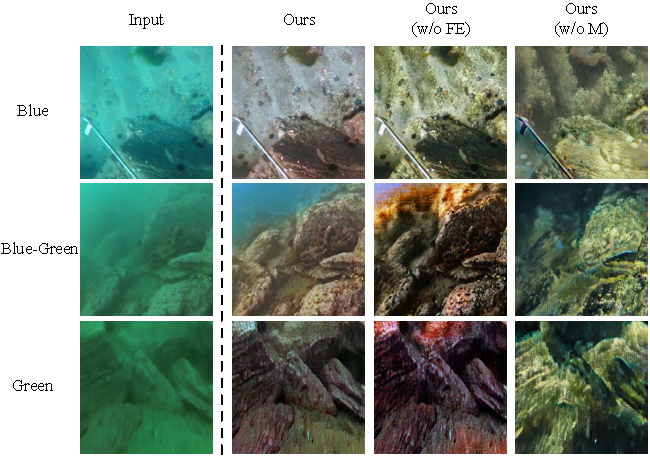
\includegraphics[width=\textwidth]{figs/RUIE_UCCS.pdf}
	\caption{我们的方法和去掉FE或M网络的方法在RUIE数据集的UCCS子集上的视觉效果。}
	\label{fig:RUIE_UCCS}
\end{figure*}

\begin{figure*}[!ht]
    \centering
	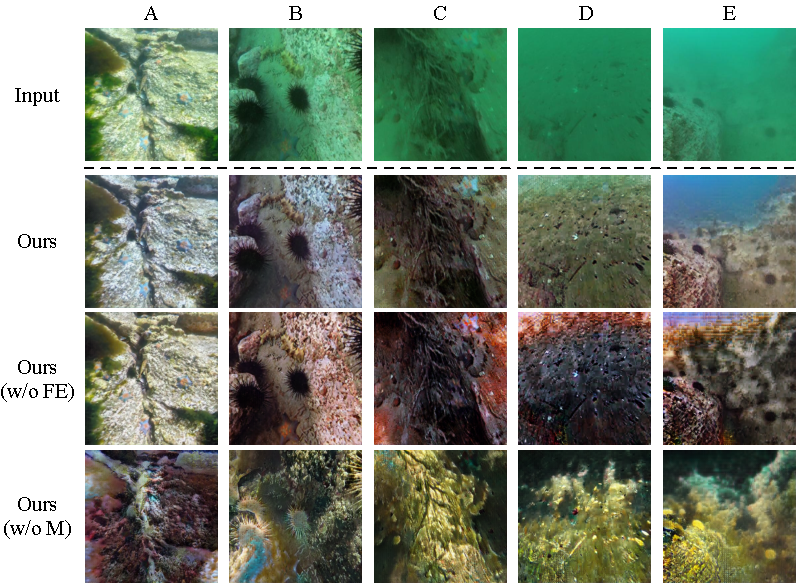
\includegraphics[width=\textwidth]{figs/RUIE_UIQS.pdf}
	\caption{我们的方法和去掉FE或M网络的方法在RUIE数据集的UIQS子集上的视觉效果。}
	\label{fig:RUIE_UIQS}
\end{figure*}

\subsubsection{映射网络的有效性验证实验}

图\ref{fig:RUIE_UCCS}和图\ref{fig:RUIE_UIQS}展示了在原有方法的基础上去掉映射网络(记作our (w/o M))的效果,如果说去掉特征提取网络使我们的网络局限于处理轻微浑浊的水下图像,那么去掉映射网络则直接导致我们的方法无法进行水下图像清晰化任务,因为从图中可以明显看出无论色调和浑浊度如何变化,去掉映射网络的方法都无法保证信息的完整性,进一步反映出在翻译前将水下信息特征与清晰图像信息空间对齐的重要性。

\section{讨论}

从前面的实验和分析中可以看出,尽管我们的方法与最先进的方法相比可以获得令人满意的结果,但仍存在几个问题:一是对于有浓雾且为开阔海域的水下图像,我们的方法不能生成很平滑的背景,推断可能是受数据集的影响,尽管训练使用的数据集是非配对的,但仍需要水下图像域和清晰图像域都包含各种场景,有浓雾且为开阔海域的水下图像容易拍摄,但这一类型的清晰图像难以获得,训练时,我们的方法在清晰域没有学习到这类图像的清晰化结果,从而影响翻译效果。二是在清晰度上仍有待加强,消融实验的结果显示去掉特征提取网络可以从浑浊程度较轻的水下图像翻译出清晰的图像,但它无法翻译浑浊水下图像,加入特征提取网络的方法则通过损失少量清晰度来实现浑浊水下图像的清晰化,后续我们会继续研究如何同时兼顾二者,以获得更清晰、适用范围更广泛的水下图像清晰化算法。

\section{本章小结}

本章将基于生成对抗网络的图像翻译应用到水下图像清晰化任务中,并针对此任务设计了我们的分解表示模型。

在第一节中,我们介绍了水下图像清晰化的意义和实用价值,以及基于生成对抗网络的方式解决清晰化问题的优势。

在第二节中,我们介绍了水下光学特性,指出水下成像受吸收和散射影响,导致水下图像存在低对比度、色偏、有雾状效果和噪声等问题。

在第三节中,我们依据水下光学特性提出我们的分解表示模型,将吸收和散射的影响分开考虑,并将分解得到的特征再映射以获得更清晰的效果。我们对再映射用到的特征提取网络和映射网络做细致描述,并介绍了所有的损失函数,最终我们给出了网络的总损失函数,实现了网络端到端的训练优化。

在第四节中,我们设计了水下图像清晰化实验,在4个数据集上证明了我们的方法的优势,并设计了消融实验,以验证特征提取网络和映射网络的有效性。

在最后一节中,我们讨论了我们的方法存在的局限性,为后续研究指明方向。





\chapter{总结与展望}

\section{总结}

本文主要对现有的基于生成对抗网络的图像翻译问题进行了深入的探讨,调研了非配对图像翻译中的循环一致性方式以及分解表示,确定二者在图像翻译问题中的应用,并尝试用其解决两个问题。对于多目标形变图像翻译问题,我们将复杂的问题分为几个小问题,并引入循环一致性思想。对于水下图像清晰化问题,我们将分解表示与水下光学特性结合考虑,提出一个基于分解表示的图像翻译模型。主要工作内容如下:

\begin{itemize}
	\item [1.]
	调研并分析了当下基于生成对抗网络的图像翻译任务的特点,并对当前最新的研究算法进行了评估,在此基础上,我们主要关注非配对图像翻译中的两个问题:一是当图像中存在多个目标且两个域之间存在较大的形状差异时,存在无法使每个目标的形状和纹理都实现翻译的问题,二是水下图像因不可避免的退化导致其存在对比度低、模糊、有雾状效果和色偏的问题。文中对每个问题都提出了一个适用的基于生成对抗网络的图像翻译模型。

	\item [2.]
	针对多目标形变图像翻译任务,我们将这一极具挑战性的问题根据形状、纹理与背景分解为三个小问题,并逐个解决,然后经一个细化网络得到最终的翻译结果。形状翻译引入非配对图像翻译中的循环一致性思想,将实例分割图从一个域翻译至另一个域,完成形状的变化,纹理翻译利用对抗损失、重建损失和颜色损失使实例分割图翻译至对应的带有纹理的前景图像,背景翻译则利用效果优异的图像修复算法,得到相对完整的背景图像,然后利用生成的实例分割图、前景图像与背景图像融合出一张完整的图像,并输入到细化网络中进行更精细的优化。

	\item [3.]
	针对水下图像清晰化任务,我们从水下图像的光学特性出发,因为水下图像的退化主要是吸收和散射共同作用的结果,所以我们基于分解表示提出了一种新的算法,将吸收导致的色偏与散射导致的雾状效果分开考虑,假设水下图像域和清晰图像域都可分解为色彩空间与信息空间,我们对清晰图像的信息特征做深层特征提取,并在翻译前使水下图像域的信息特征与清晰图像域的信息空间对齐,从而提升模型在水下图像清晰化任务上的性能。

\end{itemize}

\section{展望}

在多目标形变图像翻译任务中,虽然我们的方法可以在有较大形状差异的两个域中对多个目标实现图像翻译,但从实验结果中可以看出,我们得到的结果仍有很大的提升空间,在形状和纹理的翻译部分可以生成更细致化的结果,只有当每个部分都取得令人满意的结果,才能保证最终生成高质量的结果。另外,我们现在利用实例分割图以确定图像中目标的数量、位置和形状等信息,后续可以在目前实验取得优异结果后思考如何去掉实例分割图的限制,使多目标形变图像翻译任务不再受数据集的约束,扩大模型的适用范围。

对于水下图像清晰化任务,相比较经典的和最先进的方法,我们的方法都有一定的优势,但对于浓雾区域的清晰化仍需研究,或许可以结合空气中的去雾模型与水下成像原理,最有效的算法需要后续探讨与实验后确定,除此之外,我们还可以再提升生成图像的清晰度,探究何种方式可以在不降低去雾性能的前提下适当提高对比度。


%%% 其它部分
% \backmatter

%% 本科生要这几个索引,研究生不要。选择性留下。
% 插图索引
% \listoffigures
% 表格索引
% \listoftables
% 公式索引
% \listofequations


%% 参考文献
% 注意:至少需要引用一篇参考文献,否则下面两行可能引起编译错误。
% 如果不需要参考文献,请将下面两行删除或注释掉。
\bibliographystyle{thuthesis}
% \clearpage %目录中显示的页码正确
% \phantomsection %目录中的链接能正确跳转
% \addcontentsline{toc}{chapter}{参考文献} %目录中以章的名义添加条目
\bibliography{ref/refs}


%% 附录
% \begin{appendix}
% \chapter{外文资料原文}
\label{cha:engorg}

\title{The title of the English paper}

\textbf{Abstract:} As one of the most widely used techniques in operations
research, \emph{ mathematical programming} is defined as a means of maximizing a
quantity known as \emph{bjective function}, subject to a set of constraints
represented by equations and inequalities. Some known subtopics of mathematical
programming are linear programming, nonlinear programming, multiobjective
programming, goal programming, dynamic programming, and multilevel
programming$^{[1]}$.

It is impossible to cover in a single chapter every concept of mathematical
programming. This chapter introduces only the basic concepts and techniques of
mathematical programming such that readers gain an understanding of them
throughout the book$^{[2,3]}$.


\section{Single-Objective Programming}
The general form of single-objective programming (SOP) is written
as follows,
\begin{equation}\tag*{(123)} % 如果附录中的公式不想让它出现在公式索引中,那就请
                             % 用 \tag*{xxxx}
\left\{\begin{array}{l}
\max \,\,f(x)\\[0.1 cm]
\mbox{subject to:} \\ [0.1 cm]
\qquad g_j(x)\le 0,\quad j=1,2,\cdots,p
\end{array}\right.
\end{equation}
which maximizes a real-valued function $f$ of
$x=(x_1,x_2,\cdots,x_n)$ subject to a set of constraints.

\newtheorem{mpdef}{Definition}[chapter]
\begin{mpdef}
In SOP, we call $x$ a decision vector, and
$x_1,x_2,\cdots,x_n$ decision variables. The function
$f$ is called the objective function. The set
\begin{equation}\tag*{(456)} % 这里同理,其它不再一一指定。
S=\left\{x\in\Re^n\bigm|g_j(x)\le 0,\,j=1,2,\cdots,p\right\}
\end{equation}
is called the feasible set. An element $x$ in $S$ is called a
feasible solution.
\end{mpdef}

\newtheorem{mpdefop}[mpdef]{Definition}
\begin{mpdefop}
A feasible solution $x^*$ is called the optimal
solution of SOP if and only if
\begin{equation}
f(x^*)\ge f(x)
\end{equation}
for any feasible solution $x$.
\end{mpdefop}

One of the outstanding contributions to mathematical programming was known as
the Kuhn-Tucker conditions\ref{eq:ktc}. In order to introduce them, let us give
some definitions. An inequality constraint $g_j(x)\le 0$ is said to be active at
a point $x^*$ if $g_j(x^*)=0$. A point $x^*$ satisfying $g_j(x^*)\le 0$ is said
to be regular if the gradient vectors $\nabla g_j(x)$ of all active constraints
are linearly independent.

Let $x^*$ be a regular point of the constraints of SOP and assume that all the
functions $f(x)$ and $g_j(x),j=1,2,\cdots,p$ are differentiable. If $x^*$ is a
local optimal solution, then there exist Lagrange multipliers
$\lambda_j,j=1,2,\cdots,p$ such that the following Kuhn-Tucker conditions hold,
\begin{equation}
\label{eq:ktc}
\left\{\begin{array}{l}
    \nabla f(x^*)-\sum\limits_{j=1}^p\lambda_j\nabla g_j(x^*)=0\\[0.3cm]
    \lambda_jg_j(x^*)=0,\quad j=1,2,\cdots,p\\[0.2cm]
    \lambda_j\ge 0,\quad j=1,2,\cdots,p.
\end{array}\right.
\end{equation}
If all the functions $f(x)$ and $g_j(x),j=1,2,\cdots,p$ are convex and
differentiable, and the point $x^*$ satisfies the Kuhn-Tucker conditions
(\ref{eq:ktc}), then it has been proved that the point $x^*$ is a global optimal
solution of SOP.

\subsection{Linear Programming}
\label{sec:lp}

If the functions $f(x),g_j(x),j=1,2,\cdots,p$ are all linear, then SOP is called
a {\em linear programming}.

The feasible set of linear is always convex. A point $x$ is called an extreme
point of convex set $S$ if $x\in S$ and $x$ cannot be expressed as a convex
combination of two points in $S$. It has been shown that the optimal solution to
linear programming corresponds to an extreme point of its feasible set provided
that the feasible set $S$ is bounded. This fact is the basis of the {\em simplex
  algorithm} which was developed by Dantzig as a very efficient method for
solving linear programming.
\begin{table}[ht]
\centering
  \centering
  \caption*{Table~1\hskip1em This is an example for manually numbered table, which
    would not appear in the list of tables}
  \label{tab:badtabular2}
  \begin{tabular}[c]{|m{1.5cm}|c|c|c|c|c|c|}\hline
    \multicolumn{2}{|c|}{Network Topology} & \# of nodes &
    \multicolumn{3}{c|}{\# of clients} & Server \\\hline
    GT-ITM & Waxman Transit-Stub & 600 &
    \multirow{2}{2em}{2\%}&
    \multirow{2}{2em}{10\%}&
    \multirow{2}{2em}{50\%}&
    \multirow{2}{1.2in}{Max. Connectivity}\\\cline{1-3}
    \multicolumn{2}{|c|}{Inet-2.1} & 6000 & & & &\\\hline
    \multirow{2}{1.5cm}{Xue} & Rui  & Ni &\multicolumn{4}{c|}{\multirow{2}*{\thuthesis}}\\\cline{2-3}
    & \multicolumn{2}{c|}{ABCDEF} &\multicolumn{4}{c|}{} \\\hline
\end{tabular}
\end{table}

Roughly speaking, the simplex algorithm examines only the extreme points of the
feasible set, rather than all feasible points. At first, the simplex algorithm
selects an extreme point as the initial point. The successive extreme point is
selected so as to improve the objective function value. The procedure is
repeated until no improvement in objective function value can be made. The last
extreme point is the optimal solution.

\subsection{Nonlinear Programming}

If at least one of the functions $f(x),g_j(x),j=1,2,\cdots,p$ is nonlinear, then
SOP is called a {\em nonlinear programming}.

A large number of classical optimization methods have been developed to treat
special-structural nonlinear programming based on the mathematical theory
concerned with analyzing the structure of problems.
\begin{figure}[h]
  \centering
  \includegraphics{thu-lib-logo}
  \caption*{Figure~1\quad This is an example for manually numbered figure,
    which would not appear in the list of figures}
  \label{tab:badfigure2}
\end{figure}

Now we consider a nonlinear programming which is confronted solely with
maximizing a real-valued function with domain $\Re^n$.  Whether derivatives are
available or not, the usual strategy is first to select a point in $\Re^n$ which
is thought to be the most likely place where the maximum exists. If there is no
information available on which to base such a selection, a point is chosen at
random. From this first point an attempt is made to construct a sequence of
points, each of which yields an improved objective function value over its
predecessor. The next point to be added to the sequence is chosen by analyzing
the behavior of the function at the previous points. This construction continues
until some termination criterion is met. Methods based upon this strategy are
called {\em ascent methods}, which can be classified as {\em direct methods},
{\em gradient methods}, and {\em Hessian methods} according to the information
about the behavior of objective function $f$. Direct methods require only that
the function can be evaluated at each point. Gradient methods require the
evaluation of first derivatives of $f$. Hessian methods require the evaluation
of second derivatives. In fact, there is no superior method for all
problems. The efficiency of a method is very much dependent upon the objective
function.

\subsection{Integer Programming}

{\em Integer programming} is a special mathematical programming in which all of
the variables are assumed to be only integer values. When there are not only
integer variables but also conventional continuous variables, we call it {\em
  mixed integer programming}. If all the variables are assumed either 0 or 1,
then the problem is termed a {\em zero-one programming}. Although integer
programming can be solved by an {\em exhaustive enumeration} theoretically, it
is impractical to solve realistically sized integer programming problems. The
most successful algorithm so far found to solve integer programming is called
the {\em branch-and-bound enumeration} developed by Balas (1965) and Dakin
(1965). The other technique to integer programming is the {\em cutting plane
  method} developed by Gomory (1959).

\hfill\textit{Uncertain Programming\/}\quad(\textsl{BaoDing Liu, 2006.2})

\section*{References}
\noindent{\itshape NOTE: These references are only for demonstration. They are
  not real citations in the original text.}

\begin{translationbib}
\item Donald E. Knuth. The \TeX book. Addison-Wesley, 1984. ISBN: 0-201-13448-9
\item Paul W. Abrahams, Karl Berry and Kathryn A. Hargreaves. \TeX\ for the
  Impatient. Addison-Wesley, 1990. ISBN: 0-201-51375-7
\item David Salomon. The advanced \TeX book.  New York : Springer, 1995. ISBN:0-387-94556-3
\end{translationbib}

\chapter{外文资料的调研阅读报告或书面翻译}

\title{英文资料的中文标题}

{\heiti 摘要:} 本章为外文资料翻译内容。如果有摘要可以直接写上来,这部分好像没有
明确的规定。

\section{单目标规划}
北冥有鱼,其名为鲲。鲲之大,不知其几千里也。化而为鸟,其名为鹏。鹏之背,不知其几
千里也。怒而飞,其翼若垂天之云。是鸟也,海运则将徙于南冥。南冥者,天池也。
\begin{equation}\tag*{(123)}
 p(y|\mathbf{x}) = \frac{p(\mathbf{x},y)}{p(\mathbf{x})}=
\frac{p(\mathbf{x}|y)p(y)}{p(\mathbf{x})}
\end{equation}

吾生也有涯,而知也无涯。以有涯随无涯,殆已!已而为知者,殆而已矣!为善无近名,为
恶无近刑,缘督以为经,可以保身,可以全生,可以养亲,可以尽年。

\subsection{线性规划}
庖丁为文惠君解牛,手之所触,肩之所倚,足之所履,膝之所倚,砉然响然,奏刀騞然,莫
不中音,合于桑林之舞,乃中经首之会。
\begin{table}[ht]
\centering
  \centering
  \caption*{表~1\hskip1em 这是手动编号但不出现在索引中的一个表格例子}
  \label{tab:badtabular3}
  \begin{tabular}[c]{|m{1.5cm}|c|c|c|c|c|c|}\hline
    \multicolumn{2}{|c|}{Network Topology} & \# of nodes &
    \multicolumn{3}{c|}{\# of clients} & Server \\\hline
    GT-ITM & Waxman Transit-Stub & 600 &
    \multirow{2}{2em}{2\%}&
    \multirow{2}{2em}{10\%}&
    \multirow{2}{2em}{50\%}&
    \multirow{2}{1.2in}{Max. Connectivity}\\\cline{1-3}
    \multicolumn{2}{|c|}{Inet-2.1} & 6000 & & & &\\\hline
    \multirow{2}{1.5cm}{Xue} & Rui  & Ni &\multicolumn{4}{c|}{\multirow{2}*{\thuthesis}}\\\cline{2-3}
    & \multicolumn{2}{c|}{ABCDEF} &\multicolumn{4}{c|}{} \\\hline
\end{tabular}
\end{table}

文惠君曰:“嘻,善哉!技盖至此乎?”庖丁释刀对曰:“臣之所好者道也,进乎技矣。始臣之
解牛之时,所见无非全牛者;三年之后,未尝见全牛也;方今之时,臣以神遇而不以目视,
官知止而神欲行。依乎天理,批大郤,导大窾,因其固然。技经肯綮之未尝,而况大坬乎!
良庖岁更刀,割也;族庖月更刀,折也;今臣之刀十九年矣,所解数千牛矣,而刀刃若新发
于硎。彼节者有间而刀刃者无厚,以无厚入有间,恢恢乎其于游刃必有余地矣。是以十九年
而刀刃若新发于硎。虽然,每至于族,吾见其难为,怵然为戒,视为止,行为迟,动刀甚微,
謋然已解,如土委地。提刀而立,为之而四顾,为之踌躇满志,善刀而藏之。”

文惠君曰:“善哉!吾闻庖丁之言,得养生焉。”


\subsection{非线性规划}
孔子与柳下季为友,柳下季之弟名曰盗跖。盗跖从卒九千人,横行天下,侵暴诸侯。穴室枢
户,驱人牛马,取人妇女。贪得忘亲,不顾父母兄弟,不祭先祖。所过之邑,大国守城,小
国入保,万民苦之。孔子谓柳下季曰:“夫为人父者,必能诏其子;为人兄者,必能教其弟。
若父不能诏其子,兄不能教其弟,则无贵父子兄弟之亲矣。今先生,世之才士也,弟为盗
跖,为天下害,而弗能教也,丘窃为先生羞之。丘请为先生往说之。”
\begin{figure}[h]
  \centering
  \includegraphics{thu-whole-logo}
  \caption*{图~1\hskip1em 这是手动编号但不出现索引中的图片的例子}
  \label{tab:badfigure3}
\end{figure}

柳下季曰:“先生言为人父者必能诏其子,为人兄者必能教其弟,若子不听父之诏,弟不受
兄之教,虽今先生之辩,将奈之何哉?且跖之为人也,心如涌泉,意如飘风,强足以距敌,
辩足以饰非。顺其心则喜,逆其心则怒,易辱人以言。先生必无往。”

孔子不听,颜回为驭,子贡为右,往见盗跖。

\subsection{整数规划}
盗跖乃方休卒徒大山之阳,脍人肝而餔之。孔子下车而前,见谒者曰:“鲁人孔丘,闻将军
高义,敬再拜谒者。”谒者入通。盗跖闻之大怒,目如明星,发上指冠,曰:“此夫鲁国之
巧伪人孔丘非邪?为我告之:尔作言造语,妄称文、武,冠枝木之冠,带死牛之胁,多辞缪
说,不耕而食,不织而衣,摇唇鼓舌,擅生是非,以迷天下之主,使天下学士不反其本,妄
作孝弟,而侥幸于封侯富贵者也。子之罪大极重,疾走归!不然,我将以子肝益昼餔之膳。”


\chapter{其它附录}
前面两个附录主要是给本科生做例子。其它附录的内容可以放到这里,当然如果你愿意,可
以把这部分也放到独立的文件中,然后将其 \cs{input} 到主文件中。

% \end{appendix}

%% 致谢
% 如果使用声明扫描页,将可选参数指定为扫描后的 PDF 文件名,例如:
% \begin{acknowledgement}[scan-statement.pdf]
\begin{acknowledgement}
  现在是2021年5月7日晚9点整,再次打开sublime开始写致谢,其实这个致谢页面我打开过很多次,每次打开都会陷入浓浓的离别情绪中而无法继续。天下无不散之筵席,在研究生生涯即将结束的时候,特向所有给予我鼓励、关心和帮助的人致以最诚挚的感谢。

  饮其流者怀其源,学其成时念吾师。我要感谢我的导师郑海永教授,研究生期间能够成为您的学生是一件很幸运的事,您是良师,也是益友,从您身上我学到了很多为人处世的道理。您对于科研工作一直是高标准严要求,态度上一丝不苟,经常说“要做,就做一流的工作”。科研的道路是艰辛的,您带领着我们一路披荆斩棘,助我们成长。您对我们虽然严厉,但总是很有耐心,我经常在您的雷区疯狂跳动,但您还是会尽心尽力地教我,谢谢您没有放弃我。我还要感谢俞智斌老师,每次去问您问题,您总是不厌其烦地讲解,您对于学术的科学态度是我学习的榜样。在这里祝愿老师们身体健康、工作顺利!也祝愿实验室能够更上一层楼,越做越强!

  感谢实验室的师兄师姐师弟师妹以及同门们,感谢你们在这三年间对我的鼓励、关心和帮助。感谢我的好朋友李青芸和牛文杰,千金易得,知己难求,研究生三年能够认识你们并和你们成为闺蜜是一件很开心的事,我会想念我们一起约饭、一起喝酒、一起带着小被子去KTV通宵的日子哒,也很感谢你们在生活和科研上对我的支持和帮助,毕业后你们即将去北京和杭州,开启一段新的旅程,祝愿你们前程似锦,生活顺遂!

  感谢我的爸爸和妈妈在精神和物质上对我默默无私的支持,你们从不会阻止我前行的脚步,而是在旁辅助我,在我取得成绩时与我一同喜悦,在我受到挫折时给我安慰,在我疲惫时给我打气。感谢我的姐姐和姐夫对我的照顾,你们会在我迷茫时站在年轻一代的角度提出建议,并激励我奋力向前,无论是生活还是科研,你们都给我带来了很多帮助和乐趣。在这里祝你们永远健康、幸福、快乐,我爱你们!

  感谢国家自然科学基金面上项目“类别不平衡条件下海洋浮游生物图像精细识别及其原位应用研究”(批准号:61771440)和国家自然科学基金面上项目“海洋中小型浮游生物原位光学观测关键技术研究”(批准号:41776113)的资助。

  最后,感谢所有关心和帮助过我的人,祝愿你们永远幸福快乐!

\end{acknowledgement}


%% 个人简历
\begin{resume}

  \resumeitem{个人简历}

  1995年12月10日出生于山东省烟台市。

  2014年9月考入成都理工大学信息科学与技术学院通信工程专业,2018年6月本科毕业并获得工学学士学位。
  
  2018年8月考入中国海洋大学信息科学与工程学院电子与通信工程专业攻读硕士学位至今。

  \researchitem{发表的学术论文} % 发表的和录用的合在一起

  % 1. 已经刊载的学术论文(本人是第一作者,或者导师为第一作者本人是第二作者)
  \begin{publications}
    \item Chao Wang$^\#$, Wenjie Niu$^\#$, Yufeng Jiang$^\#$, Haiyong Zheng$^\ast$, Zhibin Yu$^\ast$, Zhaorui Gu, and Bing Zheng. Discriminative Region Proposal Adversarial Network for High-Quality Image-to-Image Translation. IJCV, 2019.
  \end{publications}
  % 2. 尚未刊载,但已经接到正式录用函的学术论文(本人为第一作者,或者
  %    导师为第一作者本人是第二作者)。

  % 3. 其他学术论文。可列出除上述两种情况以外的其他学术论文,但必须是
  %    已经刊载或者收到正式录用函的论文。
  \begin{publications} % [before=\publicationskip,after=\publicationskip]
    \item Zonghui Guo$^\#$, Liqiang Zhang$^\#$, Yufeng Jiang, Wenjie Niu, Zhaorui Gu$^\ast$, Haiyong Zheng, and Bing Zheng, Guoyu Wang. Few-shot Fish Image Generation and Classification. Global OCEANS 2020: Singapore - U.S. Gulf Coast, 2020.
  \end{publications}
  \begin{publications} 
    \item Zonghui Guo, Haiyong Zheng$^\ast$, Yufeng Jiang, Zhaorui Gu, and Bing Zheng. Intrinsic Image Harmonization. CVPR, 2021.
  \end{publications}

  \researchitem{在校期间参加的研究项目} % 有就写,没有就删除
  \begin{achievements}
    \item 国家自然科学基金面上项目:类别不平衡条件下海洋浮游生物图像精细识别及其原位应用研究(批准号:61771440)。
  \end{achievements}
    \begin{achievements}
    \item 国家自然科学基金面上项目:海洋中小型浮游生物原位光学观测关键技术研究(批准号:41776113)。
  \end{achievements}

\end{resume}


%% 本科生进行格式审查是需要下面这个表格,答辩可能不需要。选择性留下。
% 综合论文训练记录表
%\includepdf[pages=-]{scan-record.pdf}
\end{document}
